\documentclass{apuntes}

\title{Teoría de Galois}
\author{Víctor de Juan \and Pedro Valero}
\date{14/15 C1}

% Paquetes adicionales
\usepackage{tikztools}
\usepackage{fastbuild}
\usetikzlibrary{matrix,arrows}
% --------------------

\begin{document}
\pagestyle{plain}
\maketitle

\tableofcontents
\newpage

\chapter{Teoría de cuerpos}

\section{Extensiones algebraicas}

\begin{defn}[Extensión\IS de cuerpos]
Dados dos cuerpos $F$ y $E$ tales que $F⊆E$ diremos que $E$ es una extensión de $F$.

Se escribe $F⊆E$ (obviamente) o también $E/F$.
\end{defn}

\begin{defn}[Elemento\IS algebraico]
Sea $E/F$ una extensión de cuerpos (conmutativos). Se dice que un elemento $α∈E$ es algebraico sobre $F$ si existe un polinomio $h(t) ∈ F[t]$ tal que $h(α) = 0$.
\end{defn}

Por ejemplo, $ℚ⊆ℝ$ o $ℚ⊆ℂ$ son extensiones de $ℚ$. $\sqrt{2}$ es algebraico sobre $ℚ$ porque si tomo $h(t) = t^2 - 2$, entonces $h(\sqrt{2}) = 0$.

Es muy difícil encontrar números (reales o complejos) que no sean algebraicos (o trascendentes). Sin embargo hay muchísimos (es un conjunto no numerable).

\begin{prop} SI $α∈E$ es algebraico sobre $F$ existe un único polinomio mónico de grado mínimo $p(t) ∈ F[t]$ tal que $p(α) = 0$.

A $p(t)$ se le llama el polinomio mínimo o irreducible de $α$.

Además, $p(t)$ es un polinomio irreducible.
\end{prop}

\begin{proof}
Sea $h(t) ∈ F[t]$ mónico tal que $h(α) = 0$. Dividiendo $h(t)$ entre $p(t)$ podemos escribir \[ h(t) = q(t) · p(t) + r(t) \] donde $\deg(r(t)) < \deg(p(t))$. Si evalúo en $α$, tenemos que \[ h(α) = q(α)p(α) + r(α) \] pero sabemos que $h(α) = p(α) = 0$, luego obligatoriamente tiene que ser $r(α) = 0$.

La única forma de que $r(α)$ sea 0 y que además tenga menor grado que $p(t)$ es que $r(t) = 0$.

Por otra parte, tenemos que $h(t) = q(t)p(t)$, y si suponemos que $h(t)$ es de grado mínimo entre los que anulan a α, entonces $h(t) = p(t)$ luego $p$ es único.

Además, es irreducible porque si existiese $p(t) = p_1(t) p_2(t)$, tendríamos que $0 = p(α) = p_1(α) p_2(α)$. Si suponemos $p_1(α) = 0$, entonces $\deg p(t) = \deg p_1(t)$.
\end{proof}

\paragraph{Ejemplos:}

\begin{itemize}
\item Polinomio mínimo de $\sqrt{2}$ sobre $\rac \to p(t) = t²-2$ Es irreducible en $\rac$ (podemos aplicar también el criterio de Einsestein)

\item Vamos a sacar el polinomio mínimo de $x$ sobre $\fd_3(x^3)$, donde $\fd_3 = \quot{ℤ}{3ℤ}$.

La respuesta es $p(t) = t^3 - x^3$, que está en $\fd_3(x^3)[t]$, y vamos a comprobar que efectivamente es el polinomio mínimo.

Desde luego, $p(x) = 0$ luego anula a $x$. Ahora tenemos que comprobar si $p(t)$ es irreducible, que es preguntarse si tiene raíces en $\fd_3(x³)$.

Tenemos que\footnote{Aplicando el binomio de Newton y utilizando que el 3 es el 0 en este cuerpo, los términos $3a²b$ y $3ab²$ se cancelan.} $p(t) = t³ - x³ = (t - x)³$, luego $p(t)$ tiene una única raíz en $\fd_{3}(x)$, que es $x$. Sin embargo, $x\notin \fd_{3}(x³)$, así que $p(t)$ no tiene raíces en $\fd_{3}(x)$, así que $p(t)$ irreducible.

\end{itemize}


\begin{corol} El ideal \[ I = \{ h(t) ∈ F[t] \tq h(α) = 0 \} ⊆ F[t] \] coincide con $(p(t))$, es decir, con el ideal generado por los múltiplos de $p(t)$.
\end{corol}

Considero el homomorfismo $\appl{φ}{F[t]}{E}$, con \[ \img φ = k[α] = \left\lbrace\sum a_i α^i \tq a_i ∈ F \right\} ⊆ E \]

$k(α)$ es el subcuerpo de $E$ más pequeño que contiene a $F$ y a $α∈E$. De hecho \[ k(α) = \left\{ \frac{\sum a_i α^i}{\sum b_i α^i} \tq a_i, b_i ∈ F \right\} ⊆ E \]

\begin{theorem} Si $α$ es algebraico, entonces $k(α) = k[α]$, es decir, $k[α]$ es un cuerpo.
\end{theorem}

\begin{proof} Consideramos el homomorfismo $\appl{φ}{F[t]}{E}$.

Según el primer teorema de isomorfía, $F[t] / \ncl φ $ es isomorfo a $\img φ = k[α]$.

Pero $\ncl φ = I = (p(t))$. Y por ser $p(t)$ un polinomio irreducible sabemos que $F[t]/(p(t))$ es un cuerpo por lo que $\img φ = k[α]$ también lo es.
\end{proof}

Por ejemplo, $ℚ[\sqrt{2}]$ es un cuerpo, de hecho $ℚ[\sqrt{2}] = \frac{ℚ[t]}{(t^2 -2)}$. Pero, ¿cuál es el inverso de $1 + \sqrt{2}$? Es $\frac{1}{1+\sqrt{2}}$ que está en $ℚ[\sqrt{2}]$ porque lo podemos expresar como $\sqrt{2} - 1$.

En la extensión $\fd_3(t) / \fd_3 (t^3)$, con $\fd_3 = ℤ/3ℤ$, tenemos que $\fd_3(t^3) ⊆ \fd_3(t)$, y que $x^3$ es algebraico sobre $\fd_3(t^3)$ con polinomio irreducible $p(x) = x^3 - t^3$.
\newpage

\begin{defn}[Grado\IS de una extensión]
Sea $E/F$ una extensión de cuerpos.
El grado de la extensión es la dimensión de $E$ como espacio vectorial sobre $F$, es decir, \[[E:F] = \dim_FE \]
\end{defn}
\begin{example}
\begin{itemize}
\item $[\mathbb{C} : \real] = 2$ Podemos ver que $\mathbb{C} = \real(i)$ ¿Cuál es el polinomio mínimo de $i$ sobre $\real$?

$p(t) = t² + 1$
\item $[\rac(\sqrt{2}) : \rac)] = 2$, y una base es $\{1,\sqrt{2}\}$ y entonces el  polinomio mínimo es $p(t) = t²-2$.
\end{itemize}
\end{example}
En estos ejemplos se puede comprobar la siguiente proposición:

\begin{prop}
Sea $\alpha$ algebraico sobre $F$ y sea $p(t)$ su polinomio mínimo (que es irreducible).

Entonces, \[[F(\alpha) : F] = n = \deg(p(t))\]

Además, $\{1,\alpha,\alpha^2,\alpha^3,\dotsc,\alpha^{n-1}\}$ es una base de $F(\alpha)$ sobre $F$.
\end{prop}

\begin{proof}
Supongamos que los $α^i$ no son independientes. Entonces tendríamos que
\[a_0 + a_1\alpha + \dotsb + a_{n-1}\alpha^{n-1} = 0, a_i\in F, a_i \neq 0\;  \forall i\] para una cierta combinación de $a_i$.

En ese caso el polinomio $h(t) = a_0 + a_1t + \dotsb. + a_{n-1}t^{n-1}$ anularía a $\alpha$ lo que es una contradicción, porque el grado mínimo tiene que ser $n$ y en este caso es $n-1$.

Por tanto, la única opción que nos queda es que todos los $a_i$ sean 0, lo que demuestra que son independientes. Pero para que formen una base no basta con eso, además tienen que ser generadores.

Tomo $E=\gen{1,\alpha,\alpha^2,\dotsc,\alpha^{n-1},\alpha^{n},\alpha^{n+1},\dotsc}$, el espacio generado por estos $α^i$. Vamos a ver que de este conjunto de generadores me sobran a partir de $\alpha^n$.

Como $0 = p(\alpha) = a_0 + a_1\alpha + \dotsb + a_{n-1}\alpha^{n-1} + \alpha^n$, entonces $\alpha^n = -(a_0 + a_1\alpha + \dotsb + a_{n-1}\alpha^{n-1})$, es decir, podemos expresar los grados superiores como combinación lineal de los anteriores, y podríamos repetir el procedimiento con $α^k, k>n$

Por tanto hemos demostrado que  $\{1,\alpha,\alpha^2,\dotsc,\alpha^{n-1}\}$ son generadores e independientes por lo que son una base.
\end{proof}

Vamos a afianzar un poco el concepto de dimensión.
\begin{example}
\begin{itemize}
\item $[E:F] = 1$ $\dimplies E=F$.
\item $[\rac(\sqrt{2} : \rac]$= 2, por ser $p(t) = t^2 -2$ el polinomio mínimo.
%TODO no se que pretendes con esto de aquí abajo pero no parece funcionar
\item $[\rac (\sqrt{2},\sqrt{3}) % %}_{\text{ Minimo cuerpo que contiene \uparrow}}
:\rac]$=?
\end{itemize}
\end{example}

Para resolver esto vamos a utilizar la siguiente proposición:

\begin{prop}
$F \subset E_1 \subset E_2$ extensiones finitas.

Entonces $[E_2 : F] = [E_2 : E_1][E_1 : F]$.

Además, $\{y_i\}_{i=1}^n$ es una base de $E_2 / E_1$ y $\{x_j\}_{i=1}^n$  es una base de $E_1 / F$. Entonces $\{x_jy_i\}$ es una base de $E_2/F$
\end{prop}

\begin{proof}
\begin{enumerate}
\item $\{x_jy_i\}$ son generadores de $E_2 / F$.

$$\forall \alpha \in E_2 \implies \alpha = \sum_{i=1}^n b_iy_i; \ b_i\in E_1 \implies \alpha = \sum_{i=1}^n \left(\sum_j a_{ij}x_j\right) y_i = \sum a_{ij}x_jy_i; \ a_{ij}\in F$$

\item $\{x_jy_i\}$ son independientes sobre $F$.

\[0 = \sum a_{ij}x_iy_i = \sum_i \left(\sum_j a_{ij}x_j\right)y_i \implies \forall \sum_i a_{ij}x_j = 0 \overset{(1)}{\implies} a_{ij} = 0
\]

(1) Por ser $\{x_j\}$ base de $E_1$.
\end{enumerate}
\end{proof}


Para el caso anterior tenemos:

\[
\rac \subset \rac(\sqrt{2}) \subset \rac(\sqrt{2},\sqrt{3}) = \rac(\sqrt{2})(\sqrt{3})
\]

¿Podría ser $[\rac(\sqrt{2})(\sqrt{3}): \rac(\sqrt{2}) = 1 ]$?

Si lo fuera $\implies \sqrt{3} = a+b\sqrt{2} ;\, a,b\in\rac \implies 3=a^2+2b^2+2ab\sqrt{2} \implies \sqrt{2}\in \rac$.

Luego \[[\rac(\sqrt{2},\sqrt{3}): \rac] = [\rac(\sqrt{2},\sqrt{3}): \rac(\sqrt{2})] [\rac(\sqrt{2}): \rac] = 2 \times 2 =  4\]
\newpage
Veamos otro ejemplo:
\begin{example}
$[\rac(\sqrt{2} + \sqrt{3}) : \rac] \leq 4$

Utilizando $\gamma = \sqrt{2} + \sqrt{3}$ vamos a intentar calcular el polinomio mínimo, que sabemos que su grado, como máximo, es 4 (porque el grado de la extensión al ser generada por un elemento si coincidirá con el del polinomio mínimo).

$\gamma^2 = 2+3+2\sqrt{6} = 5 + 2\sqrt{6}$

$\gamma^3 = \gamma^2 · \gamma = ... = 11 \sqrt{2} + 9\sqrt{3} $

Al calcular $\gamma^4$ deberíamos encontrar una relación con las anteriores.

$\gamma^4 = ... = 49 + 20\sqrt{6}$


Ahora el procedimiento general sería resolver $a_0 + a_1\gamma + a_2 \gamma^2 + a_3\gamma^3 + \gamma^4 = 0$

En este caso no lo vamos a hacer porque combinando $\gamma^4$ y $\gamma^2$ podemos eliminar los radicales.

$\gamma^4 = -10 \gamma^2 = -1$. Esto quiere decir que $t^4 - 10t^2 + 1$ es un candidato a ser el polinomio mínimo.

Vamos a resolverlo también con el método general para otros casos más complicados.

Buscamos $p(t) = a_0+a_1\gamma+a_2\gamma^2 + a_3\gamma^3 + \gamma^4, a_i\in\rac$.

Sustituyendo  los $\gamma^i$ calculados anteriormente obtenemos: $a_0 + a_1() + a_2() + a_3 + $

\[
\begin{array}{ccc}
(1) & 0 =& a_0 + 5a_2 + 49\\
(\sqrt{2}) & 0 =& a_1 + 11a_3\\
(\sqrt{3}) & 0 =& a_1 + 9a_3\\
(\sqrt{2}\sqrt{3}) & 0 =& 2a_2 + 20
\end{array}
\]

Si resolvemos este sistema (comprobarlo) nos debería dar $a_0 = 1, a_1=a_3=0,a_2 = -10$
\end{example}
\begin{corol}
De este cálculo se deduce que \[\rac(\sqrt{2} + \sqrt{3}) \subseteq \rac(\sqrt{2},\sqrt{3}) \impliedby \gamma^3 - 9\gamma = 2\sqrt{2} \wedge \sqrt{2}\in\rac(\sqrt{2} + \sqrt{3}))\]

Como los cuerpos son iguales $\implies [\rac(\sqrt{2}+\sqrt{3}) : \rac] = 4 \implies p(t)$ es irreducible.
\end{corol}


\begin{defn}[Extensión\IS algebraica]
$E/F$ es una extensión algebraica cuando todos los elementos de $E$ son algebraicos sobre $F \dimplies \forall \alpha \in E,\, [F(\alpha) : F] < \infty$.
\end{defn}

\begin{prop}
$[E:F]<\infty \implies E/F$ es algebraica.
\end{prop}

El recíproco no es cierto, es decir, puede haber extensiones algebraicas de dimensión infinita.

\begin{example}
Dada la extensión $K = \rac(\sqrt{2},\sqrt[3]{2},\sqrt[5]{2},\dotsc,\sqrt[p]{2},\dotsc)$.

Esta extensión $K/\rac$ es algebraica porque cualquier extensión $F\subset F(\alpha_1,\alpha_2,...) = \bigcup_{n=1}^{\infty} F(\alpha_1,...,\alpha_n)$ con $\alpha_i$ algebraico sobre $F$, es algebraico.
\begin{proof}

Es fácil de comprobar, ya que $\forall \alpha \in K  = \bigcup_{n=1}^{\infty} F(\alpha_1,...,\alpha_n)$,  $\exists n \tlq \alpha \in F(\alpha_1,...,\alpha_n)$.

%TODO no entiendo de footnotes pero creo que la que has puesto aquí no se ve
$$[F(\alpha) : F] \leq$$
$$[F(\alpha_1,...,\alpha_n) : F] = [F(\alpha_1,..,\alpha_n): F(\alpha_1,..,\alpha_{n-1})] [ F(\alpha_1,..,\alpha_{n-1}) : F(\alpha_1,..,\alpha_{n-2})]...[F(\alpha_n):F] $$
$$\leq\footnote{$F(\alpha_i)\subseteq F(\alpha_1,...,\alpha_{n-i})$. Un cuerpo está contenido en el otro, entonces los grados del polinomio mínimo de cada uno cumplirán $p_1(t) \leq p_2(t)$} \prod_{i=1}^n [F(\alpha_i):F] < \infty$$

\end{proof}
Una vez hemos demostrado que es algebraica, vamos a demostrar que su dimensión es infinita.

Si tomamos $[K:\rac] \geq [ \rac(\sqrt[p]{2}):\rac] = p$ pues el polinomio irreducible de $\sqrt[p]{2}$ es $t^p - 2$.

Tenemos que $[K:\rac] \geq M$ donde $M$ es arbitrariamente grande, porque hay infinitos primos.
\end{example}

\begin{example}
\begin{itemize}
\item $[\rac(\sqrt{2}) : \rac] = 2$
\item \[[\rac(\sqrt{2},\sqrt[3]{2})] = \underbrace{[\rac(\sqrt{2},\sqrt[3]{2}):\rac(\sqrt{2})]}_{\leq 3 (1)} \underbrace{[\rac(\sqrt{2}):\rac]}_{= 2} = 2\cdot 3\]

(1) $\to [\rac(\sqrt[3]{2}): \rac] = 3 \implies  [\rac(\sqrt{2},\sqrt[3]{2}): \rac(\sqrt{2})] \leq 3$ porque el polinomio mínimo puede ser que contenga raices en $\sqrt{2}$ (entonces será menor) o puede ser que no, entonces será igual y el polinomio será $t^3-2$

\begin{itemize}
\item $[\rac : \rac(\sqrt[3]{2})] = 3$
\item $[\rac(\sqrt[3]{2}):\rac(\sqrt{2},\sqrt[3]{2})] = m \leq 2$
\item $[\rac : \rac(\sqrt{2})] = 2$
\item $[\rac(\sqrt{2}):\rac(\sqrt{2},\sqrt[3]{2})] = l \leq 3$
\end{itemize}
\[m=l \implies 3m=2l \implies\left\{ \begin{array}{cc}
m=2\\l=3\end{array}\right.\]
\end{itemize}
\end{example}

\begin{example}
$[\rac(\sqrt{2},\sqrt[3]{2},\sqrt[5]{2}):\rac] = 2\cdot 3\cdot5$

Se deja como ejercicio para el lector la comprobación siguiendo el mismo razonamiento que antes.

\end{example}

\paragraph{Conclusión:} Existen extensiones infinitas algebraicas.

\begin{corol}
Una extensión generada por elementos algebraicos es algebraica.
\end{corol}

\begin{defn}[Cuerpo\IS algebraicamente cerrado]
Sea $F$ un cuerpo.

$F$ es algebraicamente cerrado si todo polinomio $h(t) \in F(t), deg(h) \geq 1$, tiene alguna raiz en $F$.
\end{defn}
\begin{example}
$\rac,\rac(\sqrt{2}),\real$ no son algebraicamente cerrados, porque $t^2+1$ no tiene raíces. En cambio, $\mathbb{C}$ sí es algebraicamente cerrado (esto es el Teorema Fundamental del Álgebra).
\end{example}

\begin{prop}
Sea $F\subset E$ una extensión de cuerpos tal que $E$ es algebraicamente cerrado. Consideremos $\bar{F} = \{x \in E \tq x \text{ es algebraico sobre } F \}$ (o, lo que es lo mismo, $\{ x \in E \tq [F(x):F] < ∞ \}$). Entonces:

\begin{enumerate}
\item $\bar{F}$ es un cuerpo.
\item $\bar{F} / F$ es algebraica.
\item $\bar{F}$ es algebraicamente cerrado.
\end{enumerate}
\end{prop}

\begin{proof}

\begin{enumerate}
\item Sean $x,y\in\bar{F}$. Vamos a comprobar las propiedades de cuerpos: $x+y\in \bar{F},xy\in\bar{F}x^{-1}\in\bar{F}$


\begin{gather*}
x,y \in \bar{F} \implies
\begin{cases}
[F(x):F]≤ \infty\\
[F(y):F]≤ \infty
\end{cases} \implies \\
[F(x,y) :F] = \underbrace{[F(x,y) :F(y)]}_{\leq [F(x,y):F]} [F(y):F] < \infty \end{gather*}

Tenemos que $F(x,y)/F$ es algebraico. Además, $x+y,xy,x^{-1}\in F(x,y)$, por lo que $\bar{F}$ es un cuerpo.

\item $\bar{F}$ está formado por elementos algebraicos, entonces es algebraica.

\item Para demostrar que $\bar{F}$ es algebraicamente cerrado, tenemos que demostrar que cualquier polinomio $h(t) = a_0 + a_1 t + \dotsb + a_nt^n ∈ \bar{F}[t]$ (es decir, con coeficientes en $\bar{F}$) tiene raíces en $\bar{F}$. Por la propia definición, sabemos que $\bar{F} ⊆ E$ y por lo tanto sabemos que va a existir un $α∈E\tlq h(α) = 0$. Ahora bien, no sabemos si $α∈\bar{F}$ - que es lo mismo que preguntarnos si α es algebraico sobre $F$.

Consideramos la torre de cuerpos \[ F⊆F(a_0, a_1, \dotsc, a_n) ⊆ F(a_0, \dotsc, a_n;α) \]. La extensión $F(a_0, a_1, \dotsc, a_n; α) / F(a_0, \dotsc, a_n)$ es de grado menor o igual que $n$: está claro que el polinomio mínimo tendrá grado igual o menor a $h$, que ya sabemos que tiene como raíz α y tiene grado $n$.

Por otra parte, la extensión $F(a_0, a_1, \dotsc, a_n) / F$ también tiene grado finito, luego la cadena de extensiones es de grado finito y también algebraica. Esto significa que la extensión $F(a_0, a_1, \dotsc, a_n; α) / F$ es algebraica y por lo tanto α es algebraico sobre $F$, por lo que pertenece a $\bar{F}$.

Recapitulando: cualquier polinomio que encontremos en $\bar{F}$ tiene raíz α al menos en $E$. Podemos construir una extensión algebraica (finita) de cuerpos demostrando que $α$ es algebraico sobre $F$ y por lo tanto está en $\bar{F}$.
\end{enumerate}
\end{proof}

\begin{theorem}
Sea $F\subset A$ una extensión de cuerpos donde $A$ es algebraicamente cerrado.

Sea $f(t) \in F[t]$ un polinomio irreducible (en $F[t]$) de grado n.

\textbf{Entonces} $f$ tiene $n$ raices distintas en $A$.
\end{theorem}

\begin{proof}
Sabemos que $f(t) = c(t-\alpha_1) \cdot ... \cdot (t-\alpha_n)$ con $\alpha_i\in A; c\in F[t]$.

El asunto es que $\alpha_i\neq \alpha_j \forall i,j \; i\neq j $.

Vamos a demostrarlo por reducción al absurdo. Supongamos que \[\alpha_1 = \alpha_2 \implies f(t) = (t-\alpha_1)^2 \cdot q(t) \in A[t]^{(1)}\]




Consideramos la derivada $^{(2)}$: $f'(t) = 2(t-\alpha) q(t) + (t-\alpha)^2\cdot q'(t)$

Observamos que $f'(\alpha) = 0 \implies f'(t)$ es un polinomio de menor grado que $f(t)$ que anula a alpha.


Esto es: $f(t)$ \textbf{no} es el polinomio mínimo de $\alpha$ (porque hemos encontrado uno más pequeño, $f'$).

Entonces llegamos a la contradicción: $f(t)$ no es irreducible.


$^{(1)}$ $q(t)\in A[t]$ porque con el algoritmo de la división obtenemos un cociente y un resto sin salirnos del cuerpo.

$^{(2)}$ $f(t)\in F[t] \implies f'(t)\in F[t]$
\end{proof}

\begin{example}
Tomamos $[\rac\left(e^{\frac{2\pi i}{8}}\right):\rac] = 4$ (Hoja 1 Ejercicio 1 y apartado A5)

¿Es $p(t)$ irreducible? Vamos a buscarlo grado por grado.

\begin{itemize}
\item[Grado 1:] No tiene factores de grado 1 ($\dimplies$ no tiene raices).

\item[Grado 2:] $t^4+1 = (t^2 + at + b) (t^2+a't+b') = t^4 + (a+a')t^3+ (b+b'+aa') t^2 + (ab' + ba') t + bb'$

\[\implies \left\{\begin{array}{cc}
a+a' &=0\\b+b'+aa'&=0\\ab'+ba' &=0\\bb'&=1
\end{array}\right.\]

Si intentamos resolver este sistema, llegamos a la solución: $a=\sqrt{2},a'=-\sqrt{2},b=b'=\pm 1$, que no puede ser porque $\sqrt{2}\notin\rac$

\item[Grado 3:] Si tuviera un factor de grado 3 necesitaríamos otro de grado 1 que ya hemos visto que no puede ser.
\end{itemize}
\end{example}

\begin{example}[2]
\label{Teoria_H1.E1.A5.S_Af}
Tenemos $[\rac\left(e^{\frac{2\pi i}{5}}\right) : \rac]=4 \to p(t) = t^4 + t^3 + t^2 + t + 1$.

Para ello utilizamos el siguiente isomorfismos de anillos $\phi(p(t))=p(t+1)$\\ ($\appl{\Phi}{\rac[t]}{\rac[t]}$)

Por ser isomorfismo de anillos, $p(t) \;irr \dimplies \phi(p(t)) = p(t+1)\; irr$

\[\Phi(p(t)) = p(t+1) = (t+1)^4 + (t+1)^3 + (t+1)^2 + (t+1) = t^4 + 5t^3 + 10t^2 + 10t + 5\]

Con este polinomio podemos aplicar el criterio de Einsestein. Tomando $p=5$, se cumple el criterio y queda demostrado que $\Phi(p(t))$ es irreducible, por lo que $p(t)$ es irreducible (por ser $\Phi$ un isomorfismo de anillos).

\end{example}

\section{Automorfismos de cuerpos}

\begin{defn}[Inmersión]
Una inmersión de un cuerpo $F$ a un cuerpo $L$ es un homomorfismo que va de uno al otro.
\[\sigma: F \rightarrow L\]
\end{defn}

\begin{prop}
Una inmersión $\appl{σ}{F}{K}$ es siempre inyectiva.
\end{prop}
\begin{proof}
Basta ver que $\ker σ = \set{0}$.

Sea $x∈F,x≠0$. Operando, $σ(1) = 1 = σ(x · x^{-1}) = σ(x) · σ(x^{-1})$, por lo tanto $σ(x)\neq 0$.

Esto demuestra que si $x≠0$ entonces $x∉\ker σ$. Esto significa que el único elemento en $\ker σ$ es el $0$, por lo que $\sigma$ es inyectiva.
\end{proof}

\begin{defn}[Isomorfismo]
Se dice que $\appl{σ}{E}{K}$ es isomorfismo cuando además es suprayectiva.
%Corrección: Ponía automorfismo, pero un automorfismo es un isomorfismo de un cuerpo en si mismo
\end{defn}

Una inmersión $\appl{σ}{F}{K}$ induce un homomorfismo entre los correspondientes anillos de polinomios. Sea $h(t)=\sum a_i t^i$ un polinomio en $F[t]$ podemos calcular su imagen por $\sigma$ de la forma:
\[h^{\sigma}(t)=\sum a^{\sigma}_i t^i\]
con $\sigma(a_i) \in K \Rightarrow  h^{\sigma}(t) \in K[t]$, donde $h^{\sigma}(t)$ representa la imagen por $\sigma$ de $h(t)$

\begin{example}
$\appl{σ}{ℚ(i)}{ℂ}$ tal que $σ(a+bi) = a-bi$

Este homomorfismo de cuerpos induce el siguiente homomorfismo entre los anillos de polinomios.

$\appl{σ}{ℚ(i)[t]}{ℂ[t]} \implies h(t) = 3+it^2 + 6t^3 \to
h^σ = 3-it² +6t³$.
\end{example}

\paragraph{Observación importante}

Sea $α∈F$ una raiz de un polinomio $f(t): \sum a_it^i ∈F[t] \implies σ(α)$ es una raiz de $f^σ(t)$.

\begin{proof}
\[
0 = f(α) = \sum a_iα^i \implies 0=σ(0) = \sum σ(a_i)σ(α)^i = f^σ(σ(α)) = 0
\]
\end{proof}

Es decir: $σ$ envía raíces de $f(t)$ a raíces de $f^σ(t)$.

\begin{defn}[Extensión\IS de una inmersión de cuerpos]
Sea $\appl{σ}{F}{L}$ una inmersión y $E/F$ una extensión de $F$.

Una extensión de $σ$ es una inmersión (o un homomorfismo de cuerpos) $\appl{τ}{E}{L}$ tal que $τ_{|F} = σ$.

Donde $τ_{|F}$ significa $τ$ restringido a $F$.
\end{defn}

\begin{example}
Tomamos $F=ℚ,E=ℚ(i),L=ℂ$. $\appl{σ}{ℚ}{ℂ}$.

Una extensión de una inmersión implica dejar fija la actuación $\sigma$ sobre los elementos de $F$ (en este caso $\rac$). Por tanto, sólo tenemos que definir una inmersión $\appl{\sigma_1}{i}{\cplex}$, cosa que podríamos hacer de dos formas distintas: $i^{\sigma}=i$ ó $i^{\sigma}=-i$
\end{example}

\paragraph{Interesante:} Sólo hay una inmersión de $ℚ$ a cualquier cuerpo.

$\appl{σ}{ℚ}{F}$ es un homomorfismo de cuerpos. $∃! σ \tlq σ(1) = 1_F, σ(2) = 2_F$

\begin{theorem}
Sea $\appl{σ}{F}{L}$ una inmersión. Sea $p(t)∈F[t]$ irreducible.

Sea $α$ una raíz de $p(t)$ en alguna extensión $E$ de $F$ y $β$ una raíz de $p^α(t)$ en $L$.

Entonces existe una inmersión $\appl{τ}{F(α)}{L}$ que es una extensión de $σ$ con la propiedad $τ(α) = β$.

Recíprocamente, $τ$ es la extensión de $σ$ que verifica que $τ(α)$ es una raíz de $p^σ(t)$.
\end{theorem}

\begin{proof} Podemos escribir un elemento $x ∈ F(α)$ como $x = \sum a_iα^i$ con $a_i∈F$. O dicho de otra forma $x=h(α)$ siendo $h(t)$ un polinomio de $F[t]$: $h(t)=\sum a_it^i$.

Vamos a construir τ. Puesto que debe ser un homomorfismo, la única posibilidad es que ocurra lo siguiente:

\[τ(x) = τ\left(\sum a_iα^i\right) = \sum τ(a_i)τ(α)^i = \sum σ(a_i)β^i = h^σ(β)\]

Por las propiedadades de anillos, es claro que τ es un homomorfismo \textbf{siempre que esté bien definido.} Vamos a probar que es así.

Supongamos que $x=h(α) = f(α)$, donde $f(t)$ es otro polinomio en $F[t]$. Si nuestra τ está bien definida, no puede depender del polinomio $h$ que hemos tomado al inicio de la demostración y, por tanto, debemos obtener el mismo resultado si empleamos este polinomio $f$.

Tenemos que ver que $h^σ(β) = f^σ(β)$.

Si $x= h(α) = f(α) \implies α$ es raíz del polinomio $q(t) = h(t)-f(t) \implies q(t) = d(t)p(t)$, por ser $p(t)$ irreducible (por hipótesis). Todos los polinomios que se anulen en $α$ tendrán que ser múltiplos de $p(t)$ que es el irreducible.

\[q(t) = d(t)p(t) \implies q^σ(t) = d^σ(t) p^σ(t) \implies \left| \begin{array}{cc}
q^σ(β) = d^σ(β) p^σ(β) = 0&\\
\downarrow&\\
h^σ(β) - f^σ(β)=0&\implies h^σ(β) = f^σ(β)
\end{array}\right.\]
\end{proof}




%%%%%%%%%% MALVADO 2-10-2014 %%%%%%%%%%%%%

\begin{corol}
Sea $p(t) \in F[t]$ irreducible, $\sigma: F \rightarrow A$, donde A es un cuerpo algebraicamente cerrado, y sea $\alpha$ una raíz de $p(t)$ en algún cuerpo. Entonces el número de extensiones de $\sigma$ a $F(\alpha)$ es igual al número de raíces de $p(t) \eq deg(p(t))$, i.e

%%%%% Dibujo 1.1
\begin{tikzpicture}[description/.style={fill=white,inner sep=2pt}]
\matrix (m) [matrix of math nodes, row sep=3em,
column sep=2.5em, text height=1.5ex, text depth=0.25ex]
{ F & & F(α) \\
& A & \\ };
\path[->,font=\scriptsize]
(m-1-1) edge (m-1-3)
(m-1-1) edge node[description] {$ \sigma $} (m-2-2)
(m-1-3) edge node[auto] {$ \tilde{\sigma} $} (m-2-2);
\end{tikzpicture}
%%%%%%%%%%%%%%%%%%%%%%%

donde $\beta$ es cualquier raíz de $p^{\sigma}(t)$

Recordad que si $p(t) \eq a_0 + a_1t + \ldots + a_n t^n \implies p^{\sigma}(t)~=~\sigma(a_0)~+~\sigma(a_1)t~+~\ldots~+~\sigma(a_n)t^n$.
También vimos que $p(x) = 0 \implies p^{\sigma}(\tilde{\sigma}(x)) = 0$.
Para asegurar que $n \eq deg(p(t))$ estamos suponiendo que \textbf{la característica de F es 0}.


(E.G $f(t) \eq t^3 + 1 \in \fd_{3}[t] \implies f'(t) \eq 3t^2 = 0$)

\end{corol}


\begin{proof}

%%%% Dibujo 1.2
\begin{tikzpicture}[description/.style={fill=white,inner sep=2pt}]
\matrix (m) [matrix of math nodes, row sep=3em,
column sep=2.5em, text height=1.5ex, text depth=0.25ex]
{ F & & E \\
& A & \\ };
\path[->,font=\scriptsize]
(m-1-1) edge (m-1-3)
(m-1-1) edge node[description] {$ \sigma $} (m-2-2);
\draw[->, dashed] (m-1-3) -- (m-2-2);
\end{tikzpicture}

¿Cuántas $\tilde{\sigma}$'s? [E:F]

Escribo $E \eq F(\alpha_1, \alpha_2, \ldots, \alpha_k)$
%%%% Dibujo 1.3
\begin{tikzpicture}[description/.style={fill=white,inner sep=2pt}]
\matrix (m) [matrix of math nodes, row sep=3em,
column sep=2.5em, text height=1.5ex, text depth=0.25ex]
{ F & F(α_1) & F(α_1,α_2) \\
& A & \\ };
\path[->,font=\scriptsize]
(m-1-1) edge (m-1-2)
(m-1-2) edge (m-1-3)
(m-1-1) edge node[description] {$ \sigma $} (m-2-2)
(m-1-2) edge node[description] {$ \tilde{\sigma}_i $} (m-2-2)
(m-1-3) edge node[description] {$ \tilde{\sigma}_{i j} $} (m-2-2);
\end{tikzpicture}

\end{proof}

\begin{defn}[Extensión\IS separable]

Una extensión $E/F$ se llama separable si toda inmersión $\appl{σ}{F}{A}$, donde $A$ es algebraicamente cerrado, tiene exactamente $[E:F]$ extensiones.

Dicho de otra forma\footnote{AKA tal y como lo dice Wikipedia}, una extensión $E/F$ es separable si y sólo si $∀α∈E$, su polinomio mínimo es separable (tiene raíces distintas).
\end{defn}

\begin{example}
\begin{itemize}
\item Si $Ch(F)=0$, entonces $E/F$ es siempre separable.
\item $\fd_3(x^3) / \fd_3(x)$ no es separable.
\item $\fd_2(x)/\fd_2$, con $x$ tal que $x^2 = 1$, no es separable, ya que el polinomio mínimo de $x$ en $\fd_2[t]$ es $p(t) = t^2 - 1$, que si lo descomponemos en $\fd_2(x)$ es \[ t^2 - 1 = (t + x)(t-x)= (t+x)(t+x)\] por ser $1 = -1$ en $\fd_2$, y entonces tenemos raíces repetidas ($x$ es una raíz doble a pesar de que $p$ sea irreducible en $\fd_2$).\footnote{Ver más en \href{http://mathworld.wolfram.com/SeparableExtension.html}{MathWorld}.}
\item $ℚ(\sqrt[3]{2},i) / ℚ$. Ya hemos visto que $[ℚ(\sqrt[3]{2},i):ℚ] = 6$

¿Cuáles son las 6 extensiones de $\appl{j}{ℚ}{\bar{ℚ}}$?\footnote{$\bar{ℚ}$ es el cuerpo $ℚ$ extendido con algunos complejos}?


\[\begin{array}{|c|c|c|}
\hline & i & \sqrt[3]{2}\\ \hline
\hline σ_{11} & i & \sqrt[3]{2}\\
\hline σ_{12} & i & ω\sqrt[3]{2}\\
\hline σ_{13} & i & ω²\sqrt[3]{2}\\
\hline σ_{21} & -i & \sqrt[3]{2}    \\
\hline σ_{22} & -i & ω\sqrt[3]{2}   \\
\hline σ_{23} & -i & ω²\sqrt[3]{2}  \\ \hline
\end{array}
\]

$$ω  = e^{\frac{2πi}{3}}$$

$σ_{1k}(\sqrt[3]{2})$ = una raíz del polinomio $(t^3 - 2)^{σ_1} = t^3-2$

$σ_{1k}(\sqrt[3]{2})$ = una raíz del polinomio $(t^3 - 2)^{σ_2} = t^3-2$
\end{itemize}
\end{example}

\begin{theorem} \label{thmExtensionGrado} Sea $E/F$ una extensión separable finita de grado $n$, y sea $σ$ una imntesión de $F$ en un cuerpo $C$ algebraicamente cerrado sobre $F$. Entonces $σ$ tiene exactamente $n$ extensiones $\appl{τ}{E}{C}$. Es decir, hay exactamente $n$ inmersiones de $E$ en el cuerpo algebraicamente cerrado $C$ tales que la restricción $τ|_F$ de $τ$ a $F$ coincide con $σ$.

En particular, si $σ$ es la identidad en $F$, hay exactamente $n$ inmersiones de $E$ en $C$ que dejan fijo el cuerpo $F$.\footnote{Fuente: Teorema 5.18 en \href{http://www1.spms.ntu.edu.sg/~frederique/chap3.pdf}{este documento}.}
\end{theorem}
\begin{proof}

La prueba se hace por inducción. Está claro que si $n=1$, entonces $E = F$ y sólo hay una extensión $\appl{τ}{E}{C}$ tal que su restricción a $F$ sea σ, obviamente σ misma.

Supongamos ahora que $n > 1$. Sea $α∈E$, $α∉F$. Sea $f$ el polinomio mínimo de $α$ sobre $F$, y sea $r = \deg f$. Es irreducible y separable (esto es, todas sus raíces son distintas) por ser $E/F$ separable.

Consideramos la extensión $F(α)$, que cumple $F ⊂ F(α) ⊂ E$, $[E:F(α)] = n/r$ y $[F(α):F] = r$. Sea $σ$ una inmersión de $F$ en $C$ y definimos el polinomio $g = σ(f)$. Por ser σ inmersión, $g$ es irreducible y separable (todas sus raíces siguen siendo distintas). Sea β una raíz de $g$.\footnote{Ya estoy cansado, seguid la prueba en el \href{http://www1.spms.ntu.edu.sg/~frederique/chap3.pdf}{documento original (Teorema 5.18)} porque yo ya he dejado de entenderla.}
\end{proof}

\begin{defn}[Elemento\IS primitivo] \label{DefElemPrimitivo}
Dada una extensión $E/F$, si $E=F(α)$ diremos que α es un elemento primitivo.
\end{defn}

Supongamos una extensión finita $F \subset F(α,β)=E$
¿Habrá siempre un $r∈E$ tal que $E=F(γ)?$ Esto es equivalente a preguntarnos si para $E=F(α₁,...,α_n)$, existe siempre un $r$ tal que $E=F(γ)$?

\begin{example}\label{EjemploTablaExtension}
\[ ℚ(\sqrt{2},i) = ℚ(\sqrt{2} + i) \]

Como $[ℚ(\sqrt{2},i):ℚ] = 4$. También hemos visto anteriormente que la base es $\{1,i,\sqrt{2},i\sqrt{2}\}$

Siempre se prueba con $\sqrt{2} + ci$, con $c∈ℚ$. De hecho, $γ = \sqrt{2} + i$.
$$\begin{array}{ccl}
γ² &= \cdots = & 1+2i\sqrt{2} \\
γ^3 &= \cdots = &  - \sqrt{2} + 5i\\
γ^4 &= \cdots = & -7 + 4i\sqrt{2}
\end{array}$$


Vamos a hacerlo por el procedimiento largo con fines didácticos:

Buscamos un polinomio $p(t) = a₀ + a₁t + a₂t² + a_3t^3 + t⁴$ tal que $p(γ) = 0$.

$$0 = p(γ) = a₀ + a₁(\sqrt{2} + i) + a₂ (1+2i\sqrt{2}) + ...$$

Ahora escribimos los términos en función de los elementos de la base.

$$0 = (a₀ + a₂ - 7) \cdot 1 + (a₁ + 5 a_3) \cdot i + (a₁ - a_3) \cdot \sqrt{2} + (2a₂ + 4)i\sqrt{2}$$

Como tenemos una combinación lineal de elementos de una base igual a $0$, entonces los términos que multiplican tienen que ser todos 0, es decir:

$$\begin{array}{cc}
(a₀ + a₂ - 7) = 0 & \to a_0 = 9\\
(a₁ + 5 a_3) = 0 & \to a_1 = 0\\
(a₁ - a_3) = 0 & \to a_1 = a_3\\
(2a₂ + 4) = 0 & \to a_2 = -2
\end{array}$$

Entonces tenemos $p(t) = 9-2t² + t⁴$. Resolviendo esta ecuación, obtenemos: $t^2 = - \pm 2\sqrt{2} \cdot i$

Por último, tenemos que $p(t)$ es irreducible en $ℚ[t]$ porque $ℚ(γ) = ℚ(i,\sqrt{2})$

Falta comprobar esa igualdad:

$$γ + γ^3 = 6i ∈ ℚ(γ) \implies i ∈ ℚ(i+\sqrt{2}) \implies ℚ(γ,i) \subset ℚ(γ) $$

\end{example}

\begin{lemma} Sea $E/F$ una extensión finita y separable de grado $n$ y $σ_1,\dotsc,σ_n$ todas las inmersiones de $E$ en $F$. Sea $γ ∈ E$ un elemento tal que $σ_i(γ) ≠ σ_j(γ)$ si y sólo si $i ≠ j$. Entonces, $γ$ es un elemento primitivo. \end{lemma}

\begin{proof} Si la imagen de γ es distinta por todas las inmersiones $σ_i$, entonces hay al menos $n$ inmersiones $\appl{τ_i}{F(γ)}{F}$ ya que $σ_i|_{F(γ)}$ seguirá siendo inmersión. Luego, por el teorema \ref{thmExtensionGrado} tenemos que $[F(γ):F] ≥ n$. Por otra parte, $F ⊆ F(α) ⊆ E$, así que $[E:F] = [E:F(γ)]·[F(γ):F] = n$. Como $[F(γ):F] ≥ n$, sólo nos queda que $[E:F(γ)] = 1$ y por lo tanto $E = F(γ)$.
\end{proof}


\begin{theorem}[Elemento\IS primitivo]
Sea $F\hookrightarrow E = F(α₁\dotsc,α_d)$ una extensión finita. Supongamos que $\mop{Ch}(F)=0$.

Entonces, existe un elemento primitivo $γ∈E$ tal que $E=F(γ)$.
\end{theorem}


\begin{proof} Como $Ch(0) = 0$, sabemos que $E/F$ es separable. Luego, si $[E:F] = n$, entonces existen $n$ extensiones $\appl{σ₁,\dotsc,σ_n}{E}{A}$ de la inmersión $j:F\hookrightarrow A$, donde $A$ es algebraicamente cerrado.

Basta probar el resultado para $E=F(α,β)$, es decir, cuando $d=2$. Esto se debe a que $F(α₀,α₁,α₂) = F(α₀,α₁)(α₂)$ y entonces aplicamos inducción.

Basta probar que $∃c∈F\tlq$ el elemento $γ=α+cβ, c∈ℕ$ tiene la siguiente propiedad:

\begin{equation} \label{tma_pmtvo}
σ_i(γ) ≠ σ_j(γ) \dimplies i≠j
\end{equation}

y además, en ese caso $γ$ va a ser un elemento primitivo, es decir, $E=F(γ)$.

Razón:\\$[F(γ):F] = \#$\{extensiones de $\appl{j}{F}{A}$ a $F(γ) \to A$\} \footnote{Es decir, hay tantas extensiones como el grado.} $≥ n = [E:F] \implies F(γ)=E$.


Para probar \ref{tma_pmtvo} consideramos el polinomio $$f(t) = \prod_{i=1}^{n}\left[ \prod_{i≠j} (σ_j(α) - σ_i(α)) + (σ_j(β) - σ_j(β))t\right]$$

Este polinomio cumple 2 cosas: $\deg f(t) = n(n-1)$ (los dos productorio son hasta n pero el de dentro tiene 1 menos) y $f(t) ≠ 0$ (porque $σ_i ≠ σ_j$)

Como $f(t)$ no es nulo, debe existir $c∈F \tlq f(c)≠0$. Entonces, $$σ_j(α) - σ_i(α) + (σ_j(β) - σ_i(β))c≠0 \implies \underbrace{σ_j(α) + cσ_j(β)}_{\underbrace{σ(α+cβ)}_{σ(γ)}} ≠ \underbrace{σ_i(α)+cσ_i(β)}_{\underbrace{σ_i(α+cβ)}_{σ_j(γ)}}$$

Ya hemos demostrado, que para $σ_i ≠ σ_j$, además, en el valor concreto $γ$, también tenemos $σ_i(γ)≠σ_j(γ)$.

\end{proof}


\obs
\begin{itemize}
\item $γ=α+cβ$ es un elemento primitivo para algún $c∈ℤ$.
\item Para comprobar que un elemento es primitivo, basta ver que las $n$ extensiones de la inmersión/inclusión toman valores diferentes en $γ$.
\end{itemize}


\begin{example}
Encontrar un elemento primitivo de la extensión $ℚ(\sqrt[3]{2},i)$.

Ya hemos visto en \ref{EjemploTablaExtension}.

Tomamos $γ=i+\sqrt[3]{2}$. Buscamos $a_i ∈ℚ, i=1,..,5$ que hagan $a₀  + a₁γ + ... + γ^6 = 0$.

Para simplificar notación tomamos $α = \sqrt[3]{2}$.

\begin{gather*}
γ=i+α\\γ^2=-1+α²+2iα\\γ^3=-i-3α+3iα²+2\\\vdots
\end{gather*}

Da pereza seguir por este camino, asique buscamos una alternativa, con la observación anterior.

Utilizando la tabla de extensiones renombrando para tener $σ_i, i=1,..,6$. Basta comprobar que $σ_k (i+α) ≠ σ_l(i+α)\;si\;k≠l$.

\begin{gather*}
σ₁(i+cα) = i+α\\
σ₂(i+cα) = i+ωα\\
σ_3(i+cα) = i+ω²α\\
σ_4(i+cα) = -i+α\\
σ_5(i+cα) = -i+ωα\\
σ_6(i+cα) =  -i+ω²α
\end{gather*}

Sustituyendo $α,ω$ por sus valores y tomando $c=1$ comprobamos que todos son distintos, vemos que $γ=i+α$ es un elemento primitivo por el teorema, lo malo de este procedimiento es que no hemos llegado a calcular explícitamente el polinomio irreducible.
\end{example}


\section{Cuerpos de descomposición}

\begin{defn}[Cuerpo\IS de descomposición]
Sea $f(t) ∈F[t]$ un polinomio dado.

Se dice que $E/F$ es el cuerpo de descomposición de $f(t)$ si
\begin{itemize}
\item $f(t) = (t-α₁) ... (t-α_r) ∈E[t]$
\item $E=F(α₁,...,α_r)$
\end{itemize}
\end{defn}

La idea intuitiva de la definición, es añadirle al cuerpo las raices del polinomio y el nuevo cuerpo (con las raíces añadidas) se llama cuerpo de descomposición.

\begin{example}
\begin{itemize}

\item Si $F\subset ℂ$, entonces el cuerpo de descomposición de $f(t) ∈F[t]$ que factoriza en la forma $f(t) = (t-α₁) ... (t-α_r) ∈ℂ[t]$ es $E=F(α₁,...,α_r)$.

\item $ℚ(\sqrt{2})$ es el cuerpo de descomposición de $t²-2$.

\item $ℚ(i)$ es el cuerpo de descomposición de $t²+1$.

\item $ℚ(\sqrt[3]{2})$ podría ser el cuerpo de descomposición de $t³-2$, pero hay raices complejas que no están en el cuerpo, por lo que $ℚ(\sqrt[3]{2})$ no es el cuerpo de descomposición de nadie.
\end{itemize}
\end{example}

\begin{prop}
Todo polinomio $f(t) ∈ F[t]$ tiene un cuerpo $E$ de descomposición (el cuerpo en el que tiene las raíces).
\end{prop}


\begin{proof}
Vamos a demostrarlo por inducción sobre el grado del polinomio.

\textbf{Caso base: } $deg(f(t)) = 1 \implies f(t) = t-α$.  El cuerpo de descomposición $E = F(α) = F$.

\textbf{Inducción: } $deg(f(t)) ≥1$.

Escribimos $f(t) = p₁(t)p_2(t)\cdots p_r(t)$, la descomposición en factores irreducibles en $F[t]$.

Basta construir un cuerpo $K$ en el que $p_1(t)$ (irreducible en $F[t]$) tenga una raíz $α₁$  en $K[t]$ (si $p_1(t)$ tiene una raíz, entonces $f(t)$ también tiene también esa raíz).

Aplicamos inducción al polinomio $\exists g(t)∈K[t]$ definido por $f(t) = (t-α_1) \cdot g(t)$. Como $deg(g(t)) = def(f(g)) + 1$, ya podemos aplicar la inducción.

Ahora tenemos que ver que esa construcción del cuerpo es posible y se hace de la siguiente manera:

$$K = F[x]/(p_1(x))$$

¿Quién es $α₁$? Tenemos $α_1 ∈K[t]$, por lo que $α₁ = \bar{x}$ (la clase de $x$).

Razón: si $p₁(t) = a₀ + α₁t+ ...+a_dt^d$ entonces
$$p_1(\bar{x}) = α₀+α₁\bar{x} + ... + a_d\bar{x}^d = \bar{a₀ + α₁x+ ... + a_dtx^d} = \bar{p(x)} = 0$$


Para comprender esto último es necesario tener claro el anillo cociente.
\end{proof}

\begin{prop}
Supongamos que $K₁,K₂$ son dos cuerpos de descomposición de un polinomio $f(t)∈F[t]$, entonces existe un isomorfismo $\appl{φ}{K₁}{K₂}$ sobre $F$. (sobre $F$ quiere decir que extiende la aplicación inclusión/la identidad.)
\end{prop}

\begin{proof}
Vamos a demostrar un poco más, a saber, vamos a demostrar que si tenemos un isomorfismo $σ$ entre 2 cuerpos $F_1,F_2$. Para lo que nos hace  falta, $σ=id,F_1=F_2=F$, pero lo vamos a demostrar más en general.

Sean $f(t)∈F_1(t)$ y $K_1,K_2$ son cuerpos de descomposición de $f(t)$ y $f^σ(t)$ sobre $F_1,F_2$ respectivamente, entonces existe un isomorfismo $\appl{\tilde{σ}}{K₁}{K₂} \tlq \tilde{σ}_{|F_1}=σ$.

De nuevo, escribimos $f(t) = p₁(t) · \dotsb · p_r(t) ∈F_1[t]$ la descomposición en factores irreducibles en $F_1[t]$.

Tomamos una raíz $α_1∈K_1$ de $p_1(t)$. De este modo, $σ(α₁)$ será una raíz de $p_1^σ(t)$ y por tanto de $f^σ(t)$.

Sabemos que existe una extensión $\tilde{σ}$ de $σ$ del tipo:

$$
\begin{array}{ccc}
F_1&\to&F_1(α_1)\\
σ\;\downarrow&&\downarrow\;\tilde{σ}\\
F_2&\to&F_2(σ(α₁))
\end{array}
$$

A partir de aquí ya podemos razonar por inducción. ¿Cómo? Es una buena pregunta.
\end{proof}

\begin{defn}[Extensión\IS normal]
Una extensión $E/F$ se llama \textbf{normal}, si es el cuerpo de descomposición de algún polinomio $f(t) ∈ F[t]$.
\end{defn}

\begin{example}
\begin{itemize}

\item $ℚ(\sqrt{2})/ℚ$ es normal (y galoisiana, que ya veremos lo que es, pero tiene que ver con que la característica sea 0).

\item $ℚ(i) / ℚ$ es normal.

\item $ℚ(\sqrt[3]{2})/ℚ$ no es normal.

\item $\fd_3(x)/\fd_3(x³)$ es normal, porque es el cuerpo de descomposición del polinomio $t³ - x³ ∈ \fd_3(x³)[t]$ pues $t³-x³ = (t-x)³∈\fd(x)[t]$.
\end{itemize}
\end{example}

De los ejemplos anteriores, son galoisianas las 2 primeras, y las otras 2 no.

\chapter{Teoría de Galois}

\section{Teorema de Galois}

\begin{defn}[Extensión\IS galoisiana]
Una extensión $E/F$ es galoisiana si es normal y separable.
\end{defn}

%%%%%%%%%% Jorge 13-10-2014 %%%%%%%%%%%%%
\begin{defn}[Grupo\IS de Galois]
Si $E/F$ una extensión galoisiana, definimos el grupo de Galois.

\[\gal(E/F) = \left\{\appl{σ}{E}{E} \text{ automorfismo} \tq σ_{|F} = id\right\}\]
\end{defn}

Llegados a este punto y antes de seguir, vamos a recapitular algunas propiedades que ya hemos visto de forma separada pero que están relacionadas:
\begin{itemize}
\item Una extensión $E/F$ es separable $\iff$ $\forall x \in E$ el polinomio irreducible de $x$ sobre $F$ tiene todas sus raíces distintas $\iff$ El número de extensiones de una inmersión $\appl{\sigma}{F}{A}$ es $[E:F]$.
\item Si la característica de $F$ es 0, entonces la extensión $E/F$ es separable.
\item Si la extensión $E/F$ es normal y separable se dice galoisiana.
\item $\gal(E/F)=\{\appl{\sigma}{E}{E} \text{ automorfismo } \tq \sigma_{|F}=id\}$. Por tanto, si la extensión es separable sobre F, tendremos $[E:F]$ extensiones de la inmersión $\appl{\sigma}{F}{E}$ a $\appl{\sigma}{E}{E}$, que son los elementos de $\gal(E/F)$. Por tanto, queda claro que una extensión galoisiana cumple:
\[\abs{\gal(E/F)}=[E:F]\]
\end{itemize}

\begin{example}
$E = ℚ(\sqrt{2}, i)$, $F = ℚ$\\
$E/F$ es galoisiana\\
$E$ es el cuerpo de descomposición de $h(t) = (t^2-2)(t^2+1)$\\

\begin{center}
\begin{tabular}{c | c | c}
G & $\sqrt{2}$ & $i$ \\ \hline
$σ$ & $-\sqrt{2}$ & $i$ \\
$τ$ & $\sqrt{2}$ & $-i$ \\
$σ·τ$ & $-\sqrt{2}$ & $-i$ \\
$id$ & $\sqrt{2}$ & $i$ \\
\end{tabular}
\end{center}

Vemos que $|\gal(E/F)| = 4 = [E:F]$
\end{example}


\paragraph{Observación: } $E/F$ normal $\Leftrightarrow$ $E$ es el cuerpo de descomposición de algún polinomio $\Leftrightarrow$ $\forall \appl{σ}{E}{A}$, con $A$ algebraicamente cerrado, tenemos $σ(E) = E$


\begin{example}
La extensión $ℚ(\sqrt[3]{2})/ℚ$ no es normal. Supongamos una inmersión cualquiera
\[\appl{σ}{ℚ(\sqrt[3]{2})}{\overline{ℚ}}\]

Por ser inmersión, σ podría llevar $\sqrt[3]{2}$ a otras raíces del polinomio $t^3 - 2$. Por ejemplo, tomamos \[ σ(\sqrt[3]{2}) = ω = e^{\frac{2iπ}{3}}\sqrt[3]{2} \]

Sin embargo, $ω\notin ℚ(\sqrt[3]{2})$, por lo que $σ(ℚ(\sqrt[3]{2})) ≠ ℚ$ y entonces $ℚ(\sqrt[3]{2})/ℚ$ no puede ser normal.
\end{example}


\begin{theorem}[Teorema\IS fundamental de la teoría de Galois] \label{TmaFundGalois}
Sea $K/F$ una extensión galoisiana y finita. Entonces:

\begin{enumerate}
\item Hay una biyección entre los cuerpos intermedios de $K/F$ y los subgrupos del grupo de Galois $\gal(K/F)$, de la siguiente forma
\begin{align*}
\left\{E \tq F \subset E \subset K\right\} &\longleftrightarrow \{ H \tq H < \gal(K/F) \}\\
E &\longmapsto \gal(K/E) \\
K^H &\longmapsfrom H
\end{align*}

con \[K^H = \left\{x \in K \tq σ(x) = x\; \forall σ \in H \right\} \] el cuerpo de los elementos que se quedan fijos con los automorfismos de $H$.

Es decir, que dado un cuerpo $E$ le asociamos el subgrupo de los
automorfismos de $K$ que se comportan como la identidad
sobre $E$.

Y por otra parte, dado un subgrupo de los automorfismos de $K$ que fijan $F$, le asociamos el cuerpo de elementos que se quedan fijos por esos automorfismos del subgrupo.

Estas aplicaciones son inversas la una de la otra. Es decir, $K^{\gal(K/E)} = E$ y $\gal(K/K^H) = H$.

\item $\forall H < G$, la extensión $K/K^H$ es galoisiana, y $[K:K^H] = |H|$

\item $[K^H:F] = |G|/|H| = \frac{[K:F]}{|H|}$

\item $K^H/F$ es galoisiana si y sólo si $H \lhd G$.
\end{enumerate}
\end{theorem}

\begin{proof}

\paragraph{1: Existencia de la biyección} La primera afirmación dice que existe una biyección:
\begin{align*}
\left\{E \tq F \subset E \subset K\right\} &\longleftrightarrow \{ H \tq H < \gal(K/F) \}\\
E &\longmapsto \gal(K/E) \\
K^H &\longmapsfrom H
\end{align*} con \[K^H = \left\{x \in K \tq σ(x) = x\; \forall σ \in H \right\} \].

Empezamos viendo que $K^H$ es un cuerpo, porque si no no tiene sentido la afirmación. No es complicado: vamos a ver que la suma y producto de dos elementos de $K^H$ están en $K^H$ apoyándonos en el hecho de que $σ$ sea un homorfismo. Si $x,y∈K^H$, entonces $∀σ∈H$ tenemos que $σ(x) = x$ y $σ(y) = y$ por la propia definición de $H$.

Con la suma, queremos ver a dónde se nos va $x+y$. Como σ los deja fijos, $x+y = σ(x) + σ(y)$, y por ser σ homomorfismo eso es igual a $σ(x+y)$. Luego si $x+y = σ(x+y)$, la suma es un elemento que queda fijo por σ y entonces $x+y ∈ K^H$.

Con el producto el procedimiento a seguir es análogo: $x·y = σ(x)·σ(y) = σ(x·y)$, luego $x·y ∈ K^H$.

Por último, nos queda el inverso que es muy similar. $\inv{x} = \inv{σ(x)}$ que, por ser σ homeomorfismo, es igual a $σ(\inv{x})$, luego el inverso también se queda fijo y está en $K^H$. Es decir, que efectivamente $K^H$ es un cuerpo tal y como lo hemos definido.

Vamos a comprobar ahora que existe esa biyección, tenemos que comprobar que efectivamente esas dos aplicaciones que hemos definido son la inversa la una de la otra. Es decir, que podemos ``ir y volver'' de la siguiente forma \[E \longrightarrow \gal(K/E) \longrightarrow K^{\gal(K/E)} = E \]

Es decir, tenemos que demostrar la igualdad $E=K^{\gal(K/E)}$.

Veamos primero que $E \subset K^{\gal(K/E)}$. Sea $x ∈ E$, y sea $σ ∈ \gal(K/E)$. Entonces $σ(x) = x$ ya que todos los elementos de $\gal(K/E)$ fijan los elementos de $E$. Luego es claro que $x$ pertenece al cuerpo fijo de $\gal(K/E)$, y entonces $E⊆ K^{\gal()K/E)}$.

Vamos a probar ahora que $K^{\gal(K/E)} \subset E$ mediante reducción al absurdo. Supongamos que existe un elemento que está en $K^{\gal(K/E)}$ pero no en $E$, es decir, que $∃α ∈ K^{\gal(K/E)} \setminus E$.

\begin{wrapfigure}{r}{0.4\textwidth}
\centering
\inputtikz{teoria/diagrama-tfg-aptdo1}
\caption{Diagrama de la posible cadena de extensiones.}
\label{figDemTFG1}
\end{wrapfigure}

En ese caso tendríamos la cadena de extensiones de la figura \ref{figDemTFG1}, con $σ_0(α)$ otra raíz del polinomio irreducible de $α$ sobre $E$ distinta del propio α y $σ$ es una extensión de $σ_0 ∈ \gal(K/E)$.

Ahora bien, $σ(α) = σ_0(α)$ por ser una extensión y sabemos que $σ_0(α) ≠ α$, luego $σ$ no fija a $α$ y entonces $α ∉ K^{\gal(K/E)}$. Contradicción, pues teníamos como hipótesis que $α~∈~K^{\gal(K/E)}~\setminus~E$.


\paragraph{2: La extensión generada por un subgrupo de Galois es galoisiana}

Recordemos que esta afirmación decía que:

$\forall H < G$, la extensión $K/K^H$ es galoisiana, y $[K:K^H] = |H|$

Sabemos que dada una extensión $K/K^H$ galoisiana, tenemos que \[\card{\gal(K/K^H)} = [K:K^H]\], luego si $H = \gal(K/K^H)$ tenemos todo demostrado. Como siempre, demostraremos la igualdad haciendo las dobles inclusiones.

En primer lugar vamos a ver que $H \subseteq \gal(K/K^H)$. Dado un $σ ∈ H$, se tiene que $\forall x ∈ K^H$, $σ(x) = x$ por construcción de $K^H$. Por tanto, tenemos que $σ ∈ \gal(K/K^H)$ de manera bastante trivial.

Vamos a comprobar ahora la inclusión al otro lado \[ \gal(K/K^H) ⊆ H \]

Escribimos $K = F(α)$, $H= \{ σ_1, σ_2, \dotsc, σ_r\}$ y tomamos el polinomio

\begin{align*}
f(t) &= \prod_{σ∈H} (t-σ(α)) = (t-σ_1(α)) \dotsb  (t - σ_r(α)) =\\
 &= b_0 + b_1 t + \dotsb + b_{r-1} t^{r-1} + t^r ∈ K[t]
\end{align*}

Nos gustaría ver que $f(t) ∈ K^H[t]$, ya que en ese caso tendríamos que $[K : K^H] ≤ r$. Curiosamente, $K= K^H(α)$, así que sabemos calcular el grado de esta extensión: es el grado del polinomio mínimo de α en $K^H$.

Pero $f(t)$ anula a α (algún $σ∈H$ será la identidad y tendremos un factor $(t-α)$), así que entonces podemos afirmar que $[K:K^H]≤r$.

Con esto ya nos valdría: sabemos que $\card{\gal(K/K^H)} = [K:K^H] ≤ r$, y entonces tendríamos que $H = \gal(K/K^H)$.

Así que sí, queremos comprobar que $f(t) ∈ K^H[t]$. Consideramos $f^σ(t) = σ(b_0) + \dotsb + σ(b_{r-1})t^{r-1} + t^r$ $∀σ ∈ H$. Decir que $f(t) ∈ K^H[t]$ es lo mismo que decir que $f(t) = f^σ(t)$, o lo que es lo mismo, que todos los coeficientes de $f$ permanencen fijos por $σ$. Es trivial comprobarlo si miramos la expresión de $f$ como producto. En ese caso,       \[ f^σ(t) = (t-σσ_1(α)) \dotsb (t-σσ_r(α)) \], pero está claro que $\{ σσ_1, σσ_2, \dotsc, σσ_r\}$ sigue siendo $H$, luego $f(t) = f^σ(t)$. Entonces $f(t) ∈ K^H[t]$ y ya tenemos lo que necesitábamos para demostrar esta parte.


\paragraph{Última afirmación}

Tenemos que demostrar que si $F \subset E \subset K$, entonces $E/F$ es galoisiana $\dimplies H:=\gal(K/E)\lhd G $.

Esto es totalmente equivalente a demostrar que $K^H / F$ es galoisiana $\iff H \lhd G$, ya que si $H:=\gal(K/E)$ entonces $K^H$ son los elementos de $K$ fijados por los elementos de $H$, que a su vez son automorfismos de $K$ que fijan $E$, es decir: $K^H = E$.

Vamos a demostrar lo dos sentidos de la implicación
\begin{itemize}
\item Demostramos $\implies$.

Recordamos que para demostrar que un subgrupo es normal, podemos comprobar que es el núcleo de un homomorfismo, es decir, $H \lhd G \dimplies H = \ker(φ)$, con $\appl{φ}{G}{G'}$. (Esta propiedad se supone vista en \emph{Estructuras Algebraicas}).

Vamos a construir $\appl{φ}{\gal(K/E)}{\gal(E/F)}$ para después intentar ver que $\ker(φ) = H = \gal(K/E) \implies H\lhd G$

Este $φ$ lleva $φ(σ) \to σ_{|E}$ y es un homeomorfismo.
%TODO WHY?

Vamos a calcular el núcleo de este homeomorfismo para asegurarnos que es $H$.

$$\ker(φ) = \{σ∈\gal(K/F) \tq  φ(σ) = σ_{|E} = id_E = \gal(K/E)\}$$

\item Demostramos $\impliedby$

Tenemos: $F\subset E$, con $\appl{σ}{E}{K}$ y $\appl{i}{F}{K}$.

Para que sea galoisiana, tenemos que comprobar que cualquier extensión de la identidad es un automorfismo, es decir $σ(E) = E$.

Añadimos al esquema $\appl{\tilde{σ}}{K}{K}$, siendo $ F\subset K$.

Aquí sí que tenemos que $\tilde{σ}$ sí es un automorfismo, por ser $K$ extensión galoisiana.

Ahora, intentamos ver si $\tilde{σ}(E) = E$.

Para ello, es importante darnos cuenta que sabemos $\tilde{σ}H\tilde{σ}^{-1} = H$, es decir, que $H$ es normal.

En general,aunque $H$ no sea normal, tenemos: $\tilde{σ}H\tilde{σ}^{-1} = \gal(K/\tilde{σ}(E))$ (lo comprobaremos más adelante. Como tiene sentido lo vamos a tomar como cierto de momento).

Vamos a utilizar algo que ya hemos visto, que es:
Si $K$ es galoisiana cualquier cuerpo intermedio es galoisiano.

$$\gal(K/E) = H = \tilde{σ}H\tilde{σ}^{-1} = \gal(K/\tilde{σ}(E))\implies E = \tilde{σ}(E)$$

La segunda igualdad es la hipótesis, la tercera es si la suposición que tenía sentido fuera cierta y la última implicación se debe a la consecuencia 1 del Tma de Galois.

Vamos a probar que realmente la suposición
\[\tilde{σ}H\tilde{σ}^{-1} = \gal(K/\tilde{σ}(E))\]
es cierta.

Como estamos ante una igualdad, probamos 1 inclusión y comprobamos el orden de los 2 grupos.

$$\tilde{σ} H \tilde{σ}^{-1} \subset \gal(K / \tilde{σ}(E))$$

Sean $h∈H\quad z∈\tilde{σ}(E)$ arbitrarios. Basta comprobar $\tilde{σ}h\tilde{σ}^{-1} (z) = z$.

Sea $z=\tilde{σ}(x), x∈E$. Entonces:

\[\tilde{σ}h\tilde{σ}^{-1} (\tilde{σ}(x)) = \tilde{σ} h (x) = \tilde{σ}(x)\]

La segunda igualdad se debe a que $H = \gal(K/E)$ por tanto los elementos de $H$ son los automorfismos de K que cumplen $h(x) = x$ para $x \in E$.

Una vez hemos demostrado la inclusión, sólo falta probar que $|\gal(K/\tilde{σ}(E)| = |\tilde{σ}H\tilde{σ}^-1| = |H|$.

En realidad, nos bastaría ver $|\gal(K/\tilde{σ}(E)| ≤ |H|$, porque habiendo demostrado la inclusión, sabemos que no puede ser $<$.

Sabemos $$|\gal(K/\tilde{σ}(E))| =|K : \tilde{σ}(E)| \overset{(1)}{=} \frac{[K:F]}{[\tilde{σ}(E) : F]} \overset{(2)}{=} \frac{[K:F]}{[E:F]} = |\gal(K/E)| = |H|$$


$(1)$ se debe a la cadena de inclusiones, habiendo despejado.

$(2)$ se debe a que $\appl{\tilde{σ}}{E}{\tilde{σ}(E)}$ es un isomorfismo de espacios vecotriales sobre $F$.
\end{itemize}
\end{proof}

\begin{defn}[Grupo\IS de Galois de un polinomio] El grupo de Galois de un polinomio $f(t) ∈ F[t]$ es $\gal(K/F)$ donde $K$ es el cuerpo de descomposición de $f(t)$.
\end{defn}

\subsection{Ejemplos y estudio del Teorema de Galois}

\begin{example} Sean $K = ℚ(\sqrt{2}, i)$, $F = ℚ$. Consideramos \[ G = \mop{\gal}(K/F) = \gen{σ,τ} = \{id, σ, τ, στ\} \] con $σ^2 = Id$.

$G \neq C_4$ (grupo cíclico de orden 4) ya que en $G$ no tenemos un elemento de orden 4. Sin embargo $G = C_2 \times C_2$. Los subgrupos son

\begin{align*}
H_1 &= \{id\} \\
H_2 &= \gen{σ} \\
H_3 &= \gen{τ} \\
H_4 &= \gen{στ} \\
H_5 &= G
\end{align*} y los subcuerpos:

\begin{align*}
K^{H_1} &= ℚ(\sqrt{2}, i)\\
K^{H_2} &= ℚ(i)\\
K^{H_3} &= ℚ(\sqrt{2})\\
K^{H_4} &= ℚ(i\sqrt{2})\\
K^{H_5} &= ℚ
\end{align*}
\[K^{H_1} = \left\{x \in ℚ(\sqrt{2},i) \tq id(x) = x \right\} = ℚ(\sqrt{2},i)\]

\[K^{H_2} = \left\{x \in ℚ(\sqrt{2},i) \tq σ(x) = x \right\} =\]
\[= \left\{x = a + b\sqrt{2} + ci + di\sqrt{2} \tq a,b,c,d \in ℚ\ \land\ σ(x) = x\right\}=\]
\[= \left\{x = a + b\sqrt{2} + ci + di\sqrt{2} \tq σ(x) = a - b\sqrt{2} + ci - di\sqrt{2} = a + b\sqrt{2} + ci + di\sqrt{2} \right\} = \]
\[\left\{x = a + b\sqrt{2} + ci + di\sqrt{2} \tq b = 0, d = 0\right\} = \]
\[\left\{x = a + ci \tq a,c \in ℚ\right\} = ℚ(i)\]

\[K^{H_3} = K^{\gen{τ}} = \left\{x \in K \tq τ(x) = x \right\} = \left\{x = a + b\sqrt{2} + ci + di\sqrt{2} \tq τ(x) = x\right\}\]
\[= \left\{x = a + b\sqrt{2} + ci + di\sqrt{2} \tq x = τ(x) = a + b\sqrt{2} - ci - di\sqrt{2} \right\} = \]
\[\left\{x = a + b\sqrt{2} \tq a,b \in ℚ\right\} = ℚ(\sqrt{2})\]

\[K^{H_4} = \left\{x = a + b\sqrt{2} + ci + di\sqrt{2} \tq x = στ(x) = a - b\sqrt{2} - ci + di\sqrt{2}\right\} =\]
\[= \left\{x = a + di\sqrt{2} \tq a,d \in ℚ\right\} = ℚ(i\sqrt{2})\]

\[K^{H_5} = \left\{x \in K \tq σ(x) = x\ \land\ τ(x) = x \right\} =\]
\[= \left\{x \in K \tq x \in ℚ(i)\ \land\ x \in ℚ(\sqrt{2})\right\} = ℚ\]

Siguiendo con el ejemplo, ¿qué es $E = ℚ(\sqrt{2} + 7i)$?. Sabemos que $E ≠ ℚ$, entonces, ¿es $E = ℚ(\sqrt{2})$?

Si $E = ℚ(\sqrt{2})$, tendríamos que $\sqrt{2} ∈ E = ℚ(\sqrt{2} + 7i)$. Entonces $i ∈ E = ℚ(\sqrt{2} + 7i)$, luego $i ∈ E$ y entonces $E = K$. Por tanto $E ≠ ℚ(\sqrt{2})$.

¿Es $E = ℚ(i)$?. No, por lo mismo que antes. ¿Es entonces $E = ℚ(i\sqrt{2})$? Si fuera así, tendríamos que

\begin{align*}
i\sqrt{2} &∈ E \Rightarrow \\
\Rightarrow i\sqrt{2} (\sqrt{2} + 7i) &∈ E \Rightarrow \\
\Rightarrow 2i - 7\sqrt{2} &∈ E = ℚ(\sqrt{2} + 7i) \Rightarrow \\
\Rightarrow 2i - 7\sqrt{2} + 7\sqrt{2} + 7²i &∈ E \Rightarrow \\
\Rightarrow (7²+1)i ∈ E &\Rightarrow i ∈ E \Rightarrow E = K
\end{align*}

Por tanto, viendo que nuestro $E$ no es igual a ninguno de los elementos $K^H$ que cumplen $F \subset K^H \subset K$, y que siempre llegábamos a que $E=K$; podemos concluir que $ℚ(\sqrt{2} + ci) = ℚ(\sqrt{2}, i), 0 ≠ c ∈ ℚ$.

Es decir: $\sqrt{2} + ci$ es elemento primitivo de $ℚ(\sqrt{2}, i), ∀c$
\end{example}


\begin{example}
Vamos a estudiar el Teorema de Galois para $f(t) = t^4 - 2 ∈ ℚ∈[t]$. El cuerpo $K$ es el de descomposición de ese polinomio, que será el resultado de añadir todas sus raíces a $ℚ$:
\[ K = ℚ(\sqrt[4]{2}, -\sqrt[4]{2}, i\sqrt[4]{2}, -i\sqrt[4]{2}) = ℚ(i, \sqrt[4]{2}) \]

El grado de la extensión $[K:ℚ] = 8$ (para verlo, se tomaría la cadena de extensiones $ℚ \stackrel{4}{\hookrightarrow} ℚ(\sqrt[4]{2}) \stackrel{2}{\hookrightarrow} K = ℚ(\sqrt[4]{2}, i)$ con los polinomios mínimos $t^4 -2 $, $t^2+1$ respectivamente).
\newpage
\begin{wrapfigure}{r}{0.3\textwidth}
\centering
\begin{tabular}{r|c|c|c}
$\;$  & $i$ & α & orden\\\hline
$σ_1$ & $i$ &  α & 1 \\
$σ_2$ & $i$ & -α & 2 \\
$σ_3$ & $i$ & $iα$ & 4\\
$σ_4$ & $i$ & $-iα$ & 4\\\hline
$σ_5$ & $-i$ & α & 2\\
$σ_6$ & $-i$ & -α & 2\\
$σ_7$ & $-i$ & $iα$ & 2\\
$σ_8$ & $-i$ & $-iα$ & 2 \\
\end{tabular}
\caption{Automorfismos para $f(t) = t^4 - 2$.}
\label{tblGaloisT4-2}
\end{wrapfigure}

Obtengamos ahora los automorfismos que extienden la identidad. De $ℚ(i)$ a $K$ sólo tenemos los automorfismos que llevan $i$ a $i$ (automorfismo $β_1$) o a $-i$ (automorfismo $β_2$). Además, $\sqrt[4]{2}$ (que a partir de ahora llamaremos α por comodidad) debe ir a una de las raíces de $β_1(t^4-2)$. Los definimos en la tabla \ref{tblGaloisT4-2}.

\paragraph{Cuerpo fijo $K^{\gen{σ_2}}$} De aquí podemos estudiar, por ejemplo, el conjunto $K^{\gen{σ_2}}$. Si $x∈K$, entonces

\[ x = a_0 + a_1 α + a_2 α^2 + a_3 α^3 + a_4 i + a_5 iα + a_6 iα^2 + a_7iα^3 \] con los $a_i ∈ ℚ$. Si calculamos su imagen por $σ_2$, tenemos que

\[ σ_2(x) = a_0 - a_1α + a_2 α^2 -a_3 α^3 + a_4i - a_5 iα + a_6 iα^2 - a_7iα^3\] Igualando coeficientes, tenemos que si $σ_2(x) = x$, entonces $a_1 = a_3 = a_5 = a_7 = 0$.

Luego \[ x = a_0 + a_2 \sqrt{2} + a_4 i + a_6i\sqrt{2}\] es decir, $K^{\gen{σ_2}} = ℚ(i, \sqrt{2})$.

\paragraph{Orden del grupo de Galois $\gen{σ_3}$}

Para calcular el orden de los $σ$ tenemos en cuenta:
\begin{itemize}
\item El orden de $σ$ tiene que dividir al grado de la extensión
\item Si el orden de $σ = n \implies σ^n(α) = α$ y $σ^n(i)=i$ (para este caso con $α$ e $i$).
\end{itemize}

Vamos a poner de ejemplo $σ_3$.
\[σ_3^2(i) = σ_3(σ_3(i))=i \implies  σ_3^2(i)= i\]
\[σ_3^2(α) = σ_3(σ_3(α)) = σ_3(iα) = σ_3(i)σ_3(α) = i\cdot iα =-α \implies σ_3^4(α) = σ_3^2(σ_3^2(α)) = σ_3^2(-α) =  α\]

Queda claro que $ σ_3^4(α)=α$ y que $ σ_3^4(i)=i$ y por tanto el orden de este elemento es 4.

Se deja como ejercicio para el lector la comprobación de los órdenes del resto de automorfismos.


Para comprobar que el grupo generado por $σ_3$ es normal vamos a ver que:
\[σ_iσ_3σ_i^{-1} = σ_3\]

Aquí no vamos a hacerlo completo pero vamos a probar como se haría en un caso concreto (el resto se dejan como ejercicio para el lector)

El caso que vamos a estudiar es:
\[σ_5σ_3σ_5^{-1} = σ_3\]

En este caso tenemos que:
\[σ_5σ_3σ_5(i)^{-1} = σ_5σ_3(-i) = σ_5(-i) = i\]
\[σ_5σ_3σ_5(α)^{-1} = σ_5σ_3(α) = σ_5(iα) =-iα \]

Es decir, $σ_5σ_3σ_5^{-1} = σ_4 = σ_3^3$.

Tenemos: $G=\gen{σ_3σ_5 , \ σ_5σ_3 = σ_3^3σ_5}$ que es el grupo diedral, también conocido como $D_4$, del que ya hemos estudiado a fondo en la asignatura de \emph{Estructuras algebraicas}.

\paragraph{Cuerpo fijo $K^{\gen{σ_3}}$} Prosigamos con el mismo ejemplo viendo otras cosas interesantes:

Vamos a ver que:
\[[K^{\gen{σ_3}}:ℚ] = \frac{8}{4} = 2\]

Para comprobarlo vamos a construir $K^{\gen{σ_3}}$. Vemos que todo elemento de $K$ será de la forma \[ x = a₀ + a₁α + a₂α^2 + a_3α^3 + a_4i + a_5oα + a_6iα^2 +  a_7iα^3 \] y entonces su imagen por $σ_3$ es

\[ σ_3(x) = a₀ + a₁iα -a_2α^2 + a_3iα^3 + a_4i - a_5α + a_6i(-α^2) + a_7α^3 \]

Puesto que sabemos que $K^{\gen{σ_3}}$ es el conjunto de todos los elementos de $K$ que quedan fijos por $σ_3$ y tenemos la expresión general de un elemento cualquiera de $K$, veamos qué coeficientes necesitamos para que se cumpla $σ_3(x) = x$

$$σ_3(x) = x \dimplies \left\{
\begin{array}{cc}
a₀=a₀\\
a_1 = a_5\\
a_2 = -a_2 \implies a_2=0\\
a_4=a_4\\
a_5 = -a_1\\
a_6 = -a_6\\
a_7 = a_3
\end{array}
\right. \implies a_1=a_5=a_3=a_7=a_6 = 0$$

Sustituyendo, si $K^{\gen{σ_3}} = \{x∈K \tq σ(x)=x\}$ entonces \[ K^{\gen{σ_3}} = \{
x = a₀ + a_4i \tq a_0,a_4 ∈ℚ\} \], luego $K^{\gen{σ_3}} = ℚ(i)$.

La pregunta que se nos plantea ahora es si esta extensión es o no galoisiana. Sabemos que lo será puesto que tiene característica 0 y $H = K^{\gen{σ_3}}$ es subgrupo de $G$ (Observar segundo apartado del Teorema Fundamental de la teoría de Galois).

Por otro lado, también podemos probarlo por medio del cuarto apartado del mismo teorema puesto que, como ya hemos visto, se tiene:
\[\gen{σ_3} \lhd G\]

\paragraph{Cuerpo fijo $K^{\gen{σ_8}}$} Vamos a ver otro ejemplo para afianzar más los contenidos: vamos a estudiar $K^{\gen{σ_8}}$.

\[K^{\gen{σ_8}} = \{x∈K | σ_8(x) = x\} \]
Puesto que sabemos:
\[x= a₀ + a₁i + a_2 α^2 + a_3α^3 + a_4i + a_5iα + a_6iα^2 + a_7iα^3\]
Podemos escribir:
\[K^{\gen{σ_8}} = \{x∈K | σ_8(x) = ... = ... = a₀ + a₁iα - a₂α^2 + a_3iα^3 - a_4i -a_5α + a_6iα^2 + a_7α^3\]

¿Cuando ocurre que $σ_8(x) = x$? Escribimos el sistema de ecuaciones:

$$σ_8(x) = x \dimplies \left\{
\begin{array}{rrc}
a₀&=a₀\\
-a_1 &= a_5\\
-a_2 &= a_2 &\implies a_2=0\\
a_3 &= a_7\\
-a_5 &= a_1\\
a_6 &= a_6\\
a_7 &= a_3
\end{array}
\right. $$

No tenemos mucha suerte porque no se nos cancelan muchos términos.

Vamos a obtener información por otro camino. Sabemos $\ord σ_8 = 2$ (calculado en \ref{tblGaloisT4-2}), entonces $[K^{\gen{σ_8}} : ℚ] = \frac{|G|}{|σ_8|} = 4$

El cuerpo es: $$K^{\gen{σ_8}} = \{x = a₀-a_5α + a_7α^3 + a_5iα + a_6iα^2 + a_7iα^3 = a₀ -a_5(α-iα) + a_6iα^2 + a_7(α^3+iα^3)\}$$

Esto tiene sentido. Si tenemos que $(α-iα),iα^2,(α^3+iα^3)$ son independientes, entonces tenemos que el cuerpo está generado por un elemento de orden 4, que es lo que debería ser como hemos calculado antes. (Tiene orden 4 porque tenemos 4 $a_i$ distitnos)

Esta respuesta, hasta aquí, sería válida, pero a uno le gustaría poder dar un generador, es decir, encontrar $γ$ tal que $K^{\gen{σ_8}} = ℚ(γ)$.

Elegimos un posible generador de los 3 posibles (sólo hay 3 posibilidades puesto que no hay más elementos de orden 4).

Nos la jugamos con $γ=α-iα$, y obtenemos:

$$\left.\begin{array}{cc}
γ=α-iα\\
γ^2 = α^2(1-i)^2 = ... = -2iα^2 \implies iα^2∈ℚ(γ)\\
γ^3 = iα^2 \cdot γ = iα^3 + α^3 \implies iα^3 + α^3∈ℚ(γ)\end{array}\right\} \implies K^{\gen{σ_8}} = ℚ(α-iα)$$

Para comprobar por ejemplo si $iα ∈ K^{\gen{σ_8}}$ (si pertenece al cuerpo fijo) vemos que $σ_8(iα) ≠ iα$, por lo que $iα \notin K^{\gen{σ_8}}$

\paragraph{Grupo de Galois y extensión galoisiana} Vamos a estudiar la siguiente implicación, con el fin de ver si la extensión es galoisiana.

$$\gen{σ_8} \lhd G \dimplies K^{\gen{σ_8}} / \rac \text{  es galoisiana}$$

Decir que es un subgrupo normal, quiere decir que;
\[σ_i^{-1}σ_8σ_i = σ_8\quad i=1,2,...,7 \]
Ya hemos visto que $G = \gen{σ_3,σ_5}$, luego basta comprobarlo para $i=3,5$.
\[σ_3^{-1}σ_8σ_3(i) = σ_3^3σ_8σ_3(i) = σ_3^3σ_8(i) = σ_3^3(-i) = -i\]
\[σ_3^{-1}σ_8σ_3(α) = σ_3^3σ_8σ_3(α) = σ_3^3σ_8(iα) = ... = iα ≠ σ_8(α)\]

Viendo que $σ_3^{-1}σ_8σ_3(α) ≠ σ_8(α)$ concluimos que $\gen{σ_8}$ no es normal. \footnote{Revisar el cálculo, porque, aunque es del profesor, no estamos seguros de que no haya errores.}

Si hubieramos obtenido $σ_3^{-1}σ_8σ_3(α) = σ_8(α)$ y $σ_3^{-1}σ_8σ_3(i) = σ_8(i)$, tendríamos que haberlo comprobado con $σ_5$.

Ahora bien, a partir de aquí puede entrarnos una duda. Si $\gen{σ_8}$ no es un subgrupo normal de $G$, según el Teorema de Galois, tendríamos que tener que $σ_k(ℚ(α-iα)) ≠ ℚ(i-iα)$ para algún $k$.\footnote{Es decir, es lo mismo demostrar que el subgrupo no es normal a que la extensión no es Galoisiana.}

Vamos a intentar demostrar que efectivamente esto es así (de lo contrario se produciría una contradicción con el Teorema Fundamental de la Teoría de Galois), para poder dormir tranquilos.

Materializando la duda, si $σ_5(α-iα) = α + iα$, entonces deberíamos tener que $σ_5(ℚ(α-iα)) ≠ ℚ(α+iα)$. Demostrémoslo por reducción al absurdo y supongamos que $ℚ(α-iα) = ℚ(α+iα)$\footnote{No estoy nada seguro de esto. Guille.}

\[\frac{α(1-i)}{α(1+i)} ∈ℚ(α(1-i)) \implies \frac{(1-i)^2}{2} = -i\]

Tendríamos entonces que $α(1+i), i∈ℚ(α(1-i))$

Teníamos ya que $iα^2∈ℚ(α(1-i))$.

Además, $\frac{α^2i}{i} ∈ℚ(α(1-i))$, por tener que $α^2,i ∈ℚ(α(1-i))$ (si 2 elementos están en un cuerpo, su cociente también).

Por último, $α(1-i) + α(1+i) = α ∈ ℚ(α(1-i))$.

Hemos llegado a la conclusión de que $K^{\gen{σ_8}} = ℚ(α,i)$.

\paragraph{Celebración!} Ya podemos celebrar que el teorema es cierto, ya que al no ser la extensión galosiana (el subgrupo no es normal) entonces los cuerpos $σ_5(ℚ(α(i-1))) ≠ ℚ(α(1+i))$
\end{example}


\subsection{Extensiones ciclotómicas}

Vamos a ver otro tipo de ejemplos realmente interesantes en los que profundizar sobre toda la teoría de Galois.


\begin{theorem}
Si $ω=ω_n$ es una raíz primitiva n-ésima de la unidad, entonces

$$\gal(ℚ(ω)/ℚ) \simeq (ℤ/nℤ)^*$$

donde $(ℤ/nℤ)^*$ es el grupo de las unidades, esto es $ℤ/nℤ \setminus \set{0}$, el grupo de los elementos invertibles.

En particular $[ℚ(ω)/ℚ] =\card{\{\text{unidades de }(ℤ/nℤ)\}}$.
\end{theorem}

Por hacer las cosas algo más formales, vamos a escribir los isomorfismos de grupos explícitamente, con sus operaciones:

\[ \left(\gal(ℚ(ω)/ω), ○\right) \simeq \left(\quot{ℤ}{nℤ}\setminus\set{0}, *\right) \simeq \left(\quot{ℤ}{(n-1)ℤ}, +\right)\]

El último isomorfismo se da sólo si $n$ es primo.

\begin{proof}
Sea $σ∈\gal(ℚ(ω)/ω)$.

$σ(ω)$ debe ser otra raíz de $t^n - 1$. Además, debe ser una raíz del mismo orden $n$. Es decir, si $ω = e^{\frac{2πi}{8}}$, entonces no puede ser $σ(ω)  = e^{\frac{2πi}{4}}$, porque tendrían órdenes distintos.

Esto se debe a que $σ$ es un isomorfismo de cuerpos por lo que es inyectivo, lo que implica que $σ(ω)^n = 1 \dimplies σ(ω^n) = 1 \dimplies ω^n = 1$.

Entonces $σ(ω) = ω^{k_σ}$ siendo $\gcd (k_{σ},n) = 1$: el máximo común divisor de $k_σ$ y $n$ no puede ser otro que uno, porque si no $ω$ y $ω^{k_σ}$ no tendrían el mismo orden.

Esta propiedad, como antes, nos permite definir una aplicación:
\[\appl{φ}{\gal(ℚ(ω_n)/ℚ)}{(ℤ/nℤ)^*}\]

Esta aplicación es un homomorfismo.

\paragraph{Razón:}
Tal y como ya hemos hecho anteriormente, para comprobar que se trata de un homomorfismo debemos ver que:
\[φ(σ_1σ_2) = φ(σ_1) \cdot φ(σ_2)\]

Realizamos el cálculo: $σ_1σ_2 (ω) = σ_1(ω^{k_{σ_2}}) = ω^{k_{σ_1}k_{σ_2}}$.

Y obtenemos que
\[φ(σ_1σ_2) = φ(ω^{k_{σ_1}k_{σ_2}}) = k_{σ_1}k_{σ_2} = φ(σ_1)φ(σ_2)\]


Una vez hemos demostrado que es un homomorfismo, tenemos que comprobar que sea inyectiva. Para ello calculamos el núcleo:
\[\ker φ = \{σ \tq k^σ = 1 \} = \{id\} \implies \gal(ℚ(ω_n)/ℚ) \subset (ℤ/nℤ)^*\] Ahora tenemos que demostrar la otra inclusión.

Para terminar la demostración, necesitamos demostrar que es suprayectivo, o equivalentemente que:
\[φ(n) =|(ℤ/nℤ)^*| \approx | \gal(ℚ(ω_n)/ℚ) | = [ℚ(ω_n):ℚ] = \deg(p(t))\]
siendo $p(t)$ el polinomio irreducible $f_n(t)$ de $ω$ sobre $ℚ$. ($f_n(t)$ polinomio ciclotómico).



De momento sabemos que $\deg(f_n(t)) ≤ φ(n)$. Para ello, basta ver que todas las raices primitivas de la unidad ($ω^k, (k,n)=1$) son raíces de $f_n(t)$.

\paragraph{Pequeño recuerdo:\footnote{Más información en \href{http://es.wikipedia.org/wiki/Funci\%C3\%B3n\_\%CF\%86\_de\_Euler}{Wikipedia}}}
 $φ$ es una función que cuenta el número de coprimos con $n$, es decir, $φ(6) = φ(2·3) = φ(2)·φ(3) = 1·2=2$. En este caso, los coprimos con 6 son $1,5$. Para el caso especial de $n = p$, tenemos que $φ(p) = p-1$. Además, $φ(p)=p-1 \dimplies ℤ/pℤ$ es un cuerpo.


Volviendo a la demostración: $∀p$ primo, $(p,n)=1$ si $ω$ es raíz de $f_n(t)$ entonces $ω^p$ también es raíz de $f_n(t)$ (porque $k=p_1·p_r \implies ω^k = ω^{p_1·p_r} = \left((ω^{p_1})^{p_2}\right)^...$)


Tenemos $t^n - 1 = f_n(t)·h(t)$ además, $f_n(t),h(t) ∈ℤ[t]$ (por el lema de Gauss).

Por reducción al absurdo, supongamos que $ξ$ es una raíz de $f_n(t)$ y $f_n(ξ^p) ≠ 0$.

$f_n(ξ^p) ≠ 0 \implies ξ^p$ es raíz de $h(t) \implies h(ξ^p) = 0 \implies ξ$ es raíz de $h(t) \implies f_n(t)/h(t^p) \implies h(t^p) = f_n(t)·g(t) ∈ℤ[t]$.


Consideramos esto último como relación en $\fd_p[t] = ℤ/pℤ[t]$.

Obtenemos la igualdad de clases $$\overline{f_n(t)} · \overline{g(t)} = \overline{h(t^p)} = \left(\overline{h}(t)\right)^p \implies \overline{f}_n(t),\overline{h}(t) \text{ no son primos entre sí}$$

Si no son primos entre sí quiere decir que tienen algún factor común. En particular en $\bar{\fd}_p$= cuerpo algebraicamente  (veremos que existe) porque entonces $x^n-\bar{1}$ tendría raíces múltiples, pero eso no es así , como se ve mirando a su derivada $nx^{n-1}$, porque si es raíz múltiple del polinomio, será también raíz de su derivada.
\end{proof}

\paragraph{Aplicación:} $[ℚ(e^{\frac{2π}{7}} : ℚ)] = φ(7) = 6$. Esto es mucho más corto que el procedimiento anterior, en el que calculábamos un isomorfismo de anillos y demás.

Además, por ser raíz 7-ésima, anula $t^7-1 = (t-1)\underbrace{(t^6 + t^5 + t^4 + t^3 + t^2 + t + 1)}_{q(t)}$ y como tiene que tener grado 6 ($φ(7) = 6$) , el polinomio irreducible tiene que ser $q(t)$.

Para afianzar la aplicación del teorema vamos a calcular para $n=7,...,20$ \\
$[ℚ(e^{\frac{2πi}{n}}):ℚ]$ y sus polinomios irreducibles.

Para ello vamos a necesitar el siguiente colorario del teorema anterior.

\begin{corol}
$$t^n-1 = \prod_{d/n}f_d(t)$$ donde $d$ es un divisor de $n$ y por tanto el productorio recorre todos los divisores de $n$ y $f_k$ es un polinomio mónico de grado $d$.
\end{corol}

\begin{example}
Vamos a ver los ejemplos para utilizar este resultado en los que además aplicaremos conceptos del teorema de Galois para seguir profundizando. Vamos a tomar las raíces n-ésimas de la unidad.

\paragraph{n=1} $t-1 = f_1(t) $
\paragraph{n=2} $t^2-1 = f_2(t)·f_1(t) = f_2(t)·(t-1) \implies f_2(t) = \frac{t^2-1}{t-1} = t+1$
\paragraph{n=3} $t^3-1 = f_3(t)·f_1(t) = f_3(t)·(t-1) \implies f_3(t) = \frac{t^3-1}{t-1} = t^2+t+1$

\textit{Grado de la extensión:}
\[[ℚ(ω_3)/ℚ] = φ(3) = 2\]

\textit{Grupo de galois:}
\[\gal(ℚ(ω_3)/ℚ) = \left(ℤ/3ℤ\right)^* = \{σ_1,σ_2: σ_1(ω) = ω \ \wedge \  σ_2(ω) = ω^2\}\]

\paragraph{n=4} $t^4-1 = f_4(t)·\underbrace{f_2(t)}_{t+1}·\underbrace{f_1(t)}_{t-1} = f_4(t)\underbrace{(t^2-1)}_{f_2(t)f_1(t)}\implies f_4(t) = \frac{t^4-1}{t^2 -1} = t^2+1$

\textit{Grado de la extensión:}
\[[ℚ(ω_4)/ℚ] = φ(4) = 2\]

\textit{Grupo de galois:}
\[\gal(ℚ(ω_4)/ℚ)\approx (ℤ/4ℤ)^* = \left \{\begin{matrix}
σ_1=Id\\
σ_2(i) = i^3 =-i
\end{matrix}\right \}\]

\paragraph{n=5} $t^5-1 = f_5(t) f_1(t) \implies f_5(t)=\frac{t^5-1}{t-1} \implies f_5(t) = t^4+t^3+t^2+t+1$

\textit{Grado de la extensión:}
\[[ℚ(ω_5)/ℚ] = φ(5) = 4\]

\textit{Grupo de Galois:}
\[\gal(ℚ(ω_5)/ℚ) \approxeq \units{5}\]

Este grupo de galois empieza a ser interesante y vamos a estudiarlo, incluso con los subcuerpos.

Los elementos del grupo son: $σ_i(ω_5) = ω_5^i$

\textit{Cuerpos intermedios:}

\[\begin{array}{ccl} ℚ(ω_5)^{\gen{σ_1}}& \longleftrightarrow& \gen{σ_1}\\
ℚ(ω_5)^{\gen{σ_2}}& \longleftrightarrow & \gen{σ_2} \\
ℚ(ω_5)^{\gen{σ_3}}& \longleftrightarrow & \gen{σ_3} \\
ℚ(ω_5)^{\gen{σ_4}}& \longleftrightarrow & \gen{σ_2^2=σ_4} \\ \end{array}\]

Veamos ahora como se calcularían los cuerpos intermedios. Para ello tomemos por ejemplo $ℚ(ω_5)^{\gen{σ_4}}$.

Recordemos que:
\[x∈ℚ(ω_5)^{\gen{σ_4}} \iff x=σ_4(x)\]
es decir:
\[x = a_1ω_5+a_2ω_5^2+a_3ω_5^3+a_4ω_5^4 +a_5ω_5^5\]\[σ_4(x) = a_1 + a_2ω_5^4+a_3ω_5^3+a_4ω_5^2+a_5ω_5\]

recordemos que $σ(a_i)=a_i$ ya que σ sólo modifica $ω_5$

\obs En estos grupos se tiene que $σ_0=σ_5$ por lo que podemos trabajar con cualquiera de ellos, pero no deberemos coger nunca los dos puesto que estaríamos tomando al mismo elemento dos veces. Es decir, podríamos haber escrito
\[x=a_0 + a_1ω_5+a_2ω_5^2+a_3ω_5^3+a_4ω_5^4\]

Igualando los coeficientes obtenemos $a_1 = a_4$ y $a_2=a_3$, con lo que ya podemos construir el cuerpo fijo:
\[ℚ(ω_5)^{\gen{σ_4}} = \{a_1(ω+ω^4) + a_2(ω^2+ω^3), a_i∈ℚ\}\]

pero a uno le gustaría poder expresar este cuerpo en función de un único generador. Vemos que

\[ℚ(ω_5)^{\gen{σ_4}} = ℚ(ω+ω^4)\quad ω^4=ω^{-1}\]

\paragraph{n=10} $t^{10}-1 = f_{10}(t) · f_5(t) · f_2(t) · f_1(t) = f_{10}(t)\underbrace{(t^5-1)}_{f_5(t)f_1(t)}\underbrace{(t+1)}_{f_2(t)} \implies$ $$ f_{10}(t) =\frac{t^{10}-1}{(t^5-1)(t+1)} = \frac{t^5+1}{t+1} = t^4-t^3+t^2-t+1$$

\textit{Grado de la extensión:}
\[[ℚ(ω_{10})/ℚ] = φ(10) = 4\]

\textit{Grupo de Galois:}
\[\units{10} \approxeq \gal(ℚ(ω_{10})/ℚ) = \left \{\begin{matrix}
\bar{1} \longleftrightarrow σ_1(ω) = ω\\
\bar{3} \longleftrightarrow σ_3(ω) = ω^3\\
\bar{7} \longleftrightarrow σ_7(ω) = ω^7\\
\bar{9} \longleftrightarrow σ_9(ω) = ω^9
\end{matrix}\right \}\]

Este grupo es abeliano (por ser isomorfo a las unidades. En general esto lo vamos a tener siempre) y también es cíclico, ya que $\gal(ℚ(ω_{10})/ℚ) = \gen{σ_3}$. Para comprobarlo es más fácil ver que $\units{10} = \gen{\bar{3}}$

\textit{Cuerpos intermedios:}

Vamos a calcular
\[ℚ(ω_{10})^{\gen{σ_9}} \longleftrightarrow \gen{σ_3^2 = σ_9}\]

Como antes, tenemos 2 posibilidades de bases para trabajar: $B_1 = \{ω^i\tq i=0,1,2,3\}$ y $B_2 = \{ω^i\tq i=1,2,3,4\}$.

Si estamos hábiles podemos ver que $ℚ(ω_{10})^{\gen{σ_9}} = ℚ(ω_{10} +\overline{ω_{10}})$ necesariamente.

Si no lo supiéramos tendríamos que hacer el cálculo de $x=σ_9(x)$

\paragraph{n=13} $t^{13}-1 = f_{13}(t)\cdot f_1(t) \implies f_{13}(t)=\frac{t^{13}-1}{t-1} = t^{12}+t^{11}+t^{10}+...+t^2+t+1$

\textit{Grado de la extensión:}
\[[ℚ(ω_{13}) : ℚ] = φ(13) = 12\]

\textit{Grupo de Galois:}
\[G = \gal(ℚ(ω_{13}) /ℚ) \approx\units{13}\]

Como $\units{13}$ es cíclico ya que tiene un elemento de orden 12, tenemos que ver si $∃x∈G, \tq \ord(x) = 12 \dimplies \ord(x) ≥ 6 \dimplies \ord(x) ≠ 1,2,3,6$.

Estudiamos, por ejemplo $\ord(2)$.
$$\ord(2) ≠ 1,2,3,6 \text{ ya que } 2^i ≠ 1, ∀ i=1,2,3,6 \implies \ord(2) = 12 \implies \text{ cíclico } $$

\subparagraph{Subgrupos }$G \equiv \units{13}$


Con cuidado podemos ver que los subgrupos de $G$ son:
\[\gen{σ_{12}} = C_2 = \gen{σ_2^6}\]
\[\gen{σ_3} = C_3 = \gen{σ_2^3}\]
\[\gen{σ_8} = C_4 = \gen{σ_2^3}\]
\[\gen{σ_4} = C_6 = \gen{σ_2^2}\]
\[\gen{σ_2} = C_{12} = G\]

\textit{Cuerpos fijos}
Como todos los subgrupos son cíclicos (en particular, son abelianos y más concretamente  normales).

\textit{Primer cuerpo fijo:}
\[K^{\gen{σ_2}} = K^{G} = ℚ\]

\textit{Segundo cuerpo fijo}
\[K^{\gen{σ_4}} = K^{\gen{σ_2^2}} = ?\]

Para calcularo, tomamos $x = a₁ω + a₂ ω^2 + ... + a_{12} ω^{12}$ y resolvemos el sistema $σ_2^2(x) = x$.

\[σ_2^2(x) = \left\{ \begin{array}{c}a_1 = a_4 = a_3 = a_{12} = a_9 = a_{10}\\
a_2 = a_8 = a_6 = a_{11} = a_5 = a_7 \end{array}\right \}\]

Esto nos dice:

\[x∈K^{\gen{σ_4}} \dimplies a_1(\underbrace{ ω + ω^3 + ω^4 + ω^9 + ω^{10} + ω^{12}}_{β_1}) + a_2 (\underbrace{ ω^2 + ω5 + ω^6 + ω^7 + ω^8 + ω^{11}}_{β_2})\]

es decir $K^{\gen{σ_4}} = ℚ(β_1)$.

¿Y qué pasa con $ β_2$? Que ya se encuentra en el cuerpo, ya que $β_2 = 1 - β_1$ ($β_1 + β_2 = 0$ debido a que $\sum_{i=0}^{12} ω^i = 0$).

\[[K^{\gen{σ_2^2}} : ℚ] = \frac{12}{6} = 2\]

Vamos a calcular el polinomio irreducible del generador $β_1$ que será de grado 2 (el grado de la extensión).

Como el grado tiene que ser 2 tiene que tener 2 raíces. Una tiene que ser $β_1$.

Por lo que $p(t) = (t-β_1) · q(t)$, siendo $q(t)= t - λ$, donde $λ$ de momento no sabemos que es. Como tiene que ser raíz, lo lógico es pensar que sea $σ_2(β_1)$, ya que si está una raíz tiene que estar su transformada \footnote{Si $α$ es ráiz de $f(t)$, entonces $σ(α)$ es raíz de $f^σ(t)$.

En este caso, como estamos calculando cuerpos fijos, tenemos $f^σ(t) = f(t)$} quedando:
\[p(t) = (t-β_1) (t-σ_2(β_1)) = t^2 + (β_1 + σ_2(β_1))t + β_1σ_2(β_1)\]

Como $σ_2(β_1) = β_2$ y $β_1+β_2 = -1$ obtenemos:

\[p(t) = t^2 + β_1β_2\]

Entonces, $K^{\gen{σ_4}} = K^{\gen{σ_2^2}} = ℚ(β_1) = ℚ(β_2)$

\textit{Posibles dudas:}

¿Porqué,si estamos calculando el cuerpo fijo por $σ_2^2$ tomamos $σ_2(β_1)$ y no $σ_2^2(β_1)$?

Es importante darse cuenta que en este cuerpo fijo, $σ_2^2 = id$ con lo que no tendría mucho sentido $σ_2^2(β_1)$. Además, si recordamos el teorema de Galois \ref{TmaFundGalois}  tenemos que $\gal(K^{\gen{σ_2^2}} / ℚ) = \gen{σ_{|K^{\gen{σ_2^2}|}}}$

\textit{Tercer cuerpo fijo}
\[K^{\gen{σ_8}} = K^{\gen{σ_2^3}} = ?\]

Repetimos el mismo proceso, teniendo una extensión de grado 3 sobre $ℚ$.

\[σ_2^3(x) = a_1ω^8+a_2ω^3+a_3ω^{11}+a_4ω^6+a_5ω+a_6ω^9+a_7ω^4+a_8ω^{12}+a_9ω^7+a_{10}ω^{2} + a_{11} ω^{10}+a_{12}ω^5\]

\[σ_2^3(x) = x \dimplies \left\{\begin{array}{c}
a_8 = a_{12} = a_5 = a_1\\
a_2 = a_3 = a_{11} = a_{10}\\
a_4 = a_6 = a_9 = a_7
\end{array} \right.\]

Entonces:
\[x∈K^{\gen{σ_2^3}} \dimplies x = a_1 (\underbrace{ω + ω^5 + ω^8 + ω^{12}}_{β_1}) + a_2 (\underbrace{ω^2 + ω^3 + ω^{10} + ω^{11}}_{β_2}) + a_3 (\underbrace{ω^4 + ω^6 + ω^7 + ω^9}_{β_3}) \]

Aquí se nos complica el mismo cálculo que antes, ya que el polinomio tiene un grado más, asique vamos a buscar otro camino.

Como antes, $\gal(K^{\gen{σ_2^3}} / ℚ) = \gen{{σ_2}_{|K^{\gen{σ_2}}}}$. Pero, $β_2$ y $β_3$ son imágenes de $β_1$ por $σ_2$ y $σ_2^2$ respectivamente.

\[K^{σ_2^3} = ℚ(β_1)\]

\textit{Cuarto cuerpo fijo}
$$K^{id} = K = ℚ$$


\textit{Quinto cuerpo fijo}
$$ K^{\gen{σ_{12}}} = ℚ(ω+ω^{12}) = ℚ(ω^2+ω^{11}) = ...$$

Sabemos que $σ_{12}$ es la conjugación compleja como habíamos visto antes. Si no,  podemos razonar que la conjugación compleja tiene que estar en el grupo y dado que el único elemento con orden 2 es $σ_{12}$, entonces $σ_{12}$ tiene que ser la conjugación compleja.

Es por ello que el cuerpo fijo es
\[K^{\gen{σ_{12}}} = K∩ℝ = ℚ(ω+ω^{12})\]

\textit{Sexto cuerpo fijo}

\[K^{σ_3} = ?\]

Resolvemos el mismo sistema de ecuaciones que sale de igualar
\[σ_3(x) = x \implies σ_3(x) = a_1ω^3 + a_2 ω^6 + a_3 ω^9 + a_4 ω^{12} + a_5ω^2 + a_6 ω^5 + a_7ω^8 + a_8ω^{11} +\]
\[+ a_9ω + a_{10}ω^4 + a_{11}ω^7 + a_{12}ω^{10}\]

\[σ_3(x) = x \dimplies \left\{\begin{array}{c}
a_1 = a_3 = a_9\\
a_2 = a_6 = a_5\\
a_4 = a_{12} = a_{10}\\
a_7 = a_8 = a_{11}
\end{array} \right.\]

Tenemos
\[x∈K^{\gen{σ_3}} \dimplies x=a_1(ω+ω^3+ω^9) + a_2 (ω^2 + ω^5 + ω^6) + a_3(ω^4+ω^{10}+ω^{12}) + a_7(ω^7 + ω^8 + ω^{11})\]

Entonces $K^{\gen{σ_3}}$ como espacio vectorial sobre $ℚ$ tiene grado 4, y su base es
\[\{ω+ω^3+ω^9,ω^2+ω^5+ω^6,ω^4+ω^{10}+ω^{12},ω^7 + ω^8 + ω^{11}\}\]

Pero como cuerpo, está generado por un único elemento (esto dice el teorma del elemento primitivo, ya que estamos con característica 0). Además, los elementos de la base son conjugados por $σ_3$ (no conjugados complejos).

Podemos comprobar $σ(ω+ω^3+ω^9) = ω^2 + ω^5 + ω^6$ y así sucesivamente con el resto.

Concluimos que el cuerpo fijo es:
\[K^{\gen{σ_3}} = ℚ(ω+ω^3+ω^9)\]

\textit{Mismo ejercicio resuelto de otra manera} Vamos a utilizar otra base para calcular el cuerpo fijo. La base a utilizar es: $x = b_0 + b_1ω + ... + b_{11}ω^{11}$

\[σ_3(x) = b_0 + b_1ω^3+b_2ω^6+b_3ω^9+b_4ω^{12} + b_5ω^2 + b_6ω^5 + b_7ω^8 + b_8ω^{11} + b_9ω + b_{10}ω^4+b_{11}ω^7\]

Al intentar igualar $x = σ_3(x)$ nos encontramos con que no está escrita en términos de una base, ya que tiene el 1 y el $ω^{12}$. Tendríamos que recurrir a la igualdad $Σω = 1$, con lo que $ω^{12} = -(ω^{11} + ω^{10} + ... + 1)$ y seguir a partir de ahí, teniendo que hacer un cálculo mucho más largo e innecesario.

\paragraph{n=15} $ω=ω_{15}, K=ℚ(ω)$

\[p(t) = t^{15}- 1 = f_{15}(t)\underbrace{f_{3}(t)}_{t^2+t+1}\underbrace{f_5(t)f_1(t)}_{= t^5-1} = \frac{t^{15} - 1}{t^5-1}\frac{1}{t^2+t+1} =  \underbrace{\frac{(t^5)^3 - 1}{t^5 - 1}}_{t^{10} + t^5 + 1} \frac{1}{t^2+t+1} $$$$p(t) =  t^8-t^7+t^5-t^4+t^3-t+1\]

\textit{Grado de la extensión: }$[K:ℚ] = φ(15) = φ(3·5) = φ(3) · φ(5)  = 2·4 = 8$.

\textit{Grupo de Galois}  $\gal(K/ℚ) = \units{15} = \units{3} × \units{5}$

\textit{Polinomio mínimo}

$\gal(K/ℚ) = C_2×C_4$ tiene 4 elementos de orden 4 y todos los demás tienen grado 2.(salvo el neutro). Para estudiar los subgrupos, hay que tener en cuenta que no hay 1 subgrupo por elemento (aunque cada subgrupo sea el generado por un elemento, pero hay repeticiones, elementos distintos que generan el mismo subgrupo).

Vamos a ver un ejemplo: $σ_2(ω) = ω^2, σ_2^2(ω) = ω^4, σ_2^3(ω) = ω^8, σ_2^4(ω) = ω$, por lo que $\ord(σ_2) = 4$.

$σ_3(ω) = ω^3, σ_3^2(ω) = ω^9, σ_3^3(ω) = ω^{12}, σ_3{ω} = ω^{12} = σ_3^4(ω) = ω^6$, pero no puede ser que $\ord(σ_3) > 4$ ya que los elementos del grupo de Galois tienen como máximo orden 4. ¿Entonces? La respuesta es sencilla,  $σ_3$ no es un automorfismo, con lo que no pertenece al grupo de Galois.


Vamos a calcular $K^{\gen{σ_2}}$

Como $n$ no es primo, entonces utilizar la base $ω^i, 1≤i≤n$ no nos garantiza que sea más fácil. Vamos a utilizar desde $1,ω^7$ como base.



$x = a_1ω+a_2ω^2+ ... + a_7ω^7$ e igualamos $x = σ_2(x)$. Para ello, $σ_2(x) = a_0 + a_1ω^2+a_2ω^4+a_3ω^6+a_4ω^8+a_5ω^{10}+a_6ω^{12}+a_7ω^{14}$

\textit{"Esto me lleva a la necesidad de tener relaciones. (Silencio) de buscar relaciones, porque tenerlas nunca las tengo, aunque puede ser que con estas matemáticas si las consiga."} El necesitar estas relaciones se debe a que no podemos igualar coeficicientes ya que no tenemos una base en ambos lados. Asique, utilizando el polinomio mínimo, escribimos
\[ω^8 = ω^7 - ω^5 + ω^4 - ω^3 + ω - 1\]
\[ω^9 = ω^8ω = ω^8 - ω^6 + ω^5 -ω^4+ω^2-ω = (ω^7 - ω^5 + ω^4 - ω^3 + ω - 1) - ω^6 + ω^5 -ω^4+ω^2-ω =\]
\[= ω^7-ω^6-ω^3+ω^2-1\]
y así sucedaneamente... $ω^{10} = ω^9ω$ y seguimos sustituyendo continuamente, para acabar expresando $σ_2$ en función de $ω^i, i≤7$ y poder igualar coeficientes. Aunque tenemos más relaciones, como $(t^{15}-1) = (t^5-1)(t^{10}+t^5+1) \implies ω^{10} = -ω^5 -1$.

Terminando este proceso (que se deja como ejercicio para el lector) llegamos a

 $σ_2(x) = a_0 + a_1ω^2+α_2ω^4+a_3ω^6+a_4(ω^7-ω^5+ω^4-ω^3+ω-1) -\\a_5 (ω^5+1) - a_6(ω^7+ω^2) + a_7(-ω^7+ω^6 -ω^4+ω^3- ω^2+1)$


 $ σ_2(x)=(a_0-a_4-a_5+a_7) + a_4ω + (a_1-a_6-a_7)ω^2 + (-a_4+a_7)ω^3 +\\(a_2+a_4-a_7) ω^4 + (-a_4-a_5)ω^5 + (a_3+a_7)ω^6 + (a_4-a_6-a_7)ω^7$


Ahora ya estamos en condiciones de igualar. Antes de ello, recordamos que como tenemos grado 2 en la extensión, solo tendremos 2 coeficientes $a_i$, asique más nos vale que solo queden 2: $$\begin{array}{cl}
a_0=a_0-a_4-a_5+a_7&\implies (a_4=a_7)\implies a_5=0\\
a_1=a_4&\\
a_2=a_1-a_6-a_7&\implies a_2=a_7\\
a_3=-a_4+a_7& \implies a_3 = -a_1+a_2 = -2a_1 \implies a_3=4a_5\\
a_4=a_2+a_4-a_7 & \implies a_2 = a_7\\
a_5= -a_4-a_5 &\implies a_5 = \frac{-a_1}{2}\\
a_6 = a_3+a_7 & \implies a_6 = -a_1+a_2+a_2 = a_1\implies 2a_2=2a_1 \\
\implies & \implies a_1=a_2=a_4=a_6=a_7\\
a_7=a_4-a_6-a_7& \implies a_4=a_6=a_1\\
\end{array}$$

Tenemos $a_3=a_5=0$ y todos los demás iguales entre ellos. Esto puede ser que sea un poco raro, ya que decíamos que tiene que tener grado 2, con lo que se ha producido algún error...

La solución es $K^{\gen{σ_2}} = ℚ\left(ω+\frac{ω}{2} - \frac{ω^3}{2} + ω^4 - \frac{ω^5}{2} + \frac{ω^7}{2}\right)$

La comprobación de que está bien es $σ_2(γ) =γ$, ya que para algo es un cuerpo fijo.
\end{example}

\chapter{Solubilidad por radicales}

En este tema, vamos a suponer siempre característica 0. Aprovechamos para recordar que todo cuerpo de característica 0 contiene a $ℚ$.


\begin{defn}[Soluble por radicales]
Sea $f(t) ∈F[t]$. Es soluble por radicales si su cuerpo de descomposición $E$ está contenido en una extensión galoisiana $K/F$ con la siguiente propiedad:

\begin{itemize}
\item Existe una sucesión de subcuerpos de $K$ de la forma $F_0 \subset F_1 \subset \dotsb \subset F_m = K$ tal que
\begin{itemize}
\item[a)] $F_{i+1} = F_i(α_{i+1})$ con $(α_{i+1})^{d_i} = a_i ∈F_i$
\item[b)] si $d = \mop{mcm} (d_1,d_2,\dotsc ,d_m)$ entonces $F_1$ contiene una raíz primitiva d-ésima de la unidad.

\end{itemize}
\end{itemize}
\end{defn}

Vamos a ver porqué esta definición refleja lo que entendemos por solubilidad por radicales intuitivamente (que es que existe una fórmula como la de $x=\frac{-b\pm\sqrt{ b^2-4ac}}{2a}$)

Si $α$ es raíz de $f(t)$, entonces $α∈E\subset K$, luego $α$ está en alguno de esos cuerpos intermedios $F_i$. Sea $l$ tal que $α∈F_l$. Para simplificar y ejemplificarlo bien, tomamos $l = 3$.

Si $α \in F_3 \implies α∈F_2(α_3)  \implies α = b_0 + b_1\sqrt[d_2]{a_2} + b_d\sqrt[d_2]{a_2^2} + ...\quad b_i∈F_2$

Puesto que $b_i \in F_2$
\[b_0 \in F_2 \implies b_0 \in F_1(α_2)= c_0 + c_1 \sqrt[d_1]{a_1} + c_2\sqrt[d_1]{} + ...\]

Y podemos hacer lo mismo con el resto de $b_i \in F_2$ con lo que llegamos a:
\[α = (c_0 + c_1 \sqrt[d_1]{a_1} + c_2\sqrt[d_1] + ...) + + (c'_0 + c'_1 \sqrt[d_1]{a_1} + c'_2\sqrt[d_1] + ...)\sqrt[d_2]{q_0 + q_1\sqrt[d_1]{a_2} + ...}+ \]
\[ + (c_0'' + c_1'' \sqrt[d_1]{a_1} + c_2''\sqrt[d_1] + ...) \sqrt[d_2]{(q_0 + q_1\sqrt[d_1]{a_2} + ...)^2}  + ...\]

Y después de volverte muy loco, puedes construir $α$ como sumas y productos de raíces.

\section{Teorema de Resolubilidad}
Vamos a ver una proposición necesaria para el teorema que veremos a continuación:

\begin{prop}
Sea $K_2 = K₁(γ)$ donde $γ$ es raíz de $t^k - a ∈K_1[t]$. Supongamos que contiene una raíz primitiva k-ésima de la unidad (ω). \textbf{Entonces: }

$$\gal(K_2/K_1) \text{ es abeliano.}$$
\end{prop}

\begin{proof}
Sea $σ∈\gal(K_2/K_1)$.

Sea $ω$ una raíz primitiva k-ésima de la unidad.

Entonces $σ(γ) = ω^{d_σ}γ$ para algún $d_σ ∈ ℤ$ ya que los automorfismos del grupo de Galois mandan raíces del polinomio en raíces del polinomio.

Más concretamente sabemos que $d_σ∈ℤ/kℤ$, ya que $ω^k = 1$.

Definimos $\appl{φ}{\gal(K_2/K_1)}{ℤ/kℤ}$ que para cada $\sigma$ nos $d_{\sigma}$ tal que $σ(γ) = ω^{d_σ}γ$.

Vamos a comprobar que se trata de un homomorfismo de grupos, para ello necesitamos asegurarnos de que dados $σ_1,σ_2$ se cumple:

\[φ(σ_1σ_2) =  φ(σ_1) + φ(σ_2)\]

Calculamos $σ_1σ_2(γ) = σ_1(σ₂(γ)) = σ_1(ω^{d_{σ_2}}γ) = ω^{d_{σ_2}}σ_1(γ) = ω^{d_{σ_2}} ω^{d_{σ_1}} γ$

Por tanto, tenemos que $φ(σ_1σ_2) = d_{σ_1} + d_{σ_2} = φ(σ_1) + φ(σ_2)$ quedando claro así que se trata de un homomorfismo de grupos.


Recordamos que para que, además, sea un isomorfismo, necesitamos $\ker(φ)$ sea el trivial (sólo contenga al elemento neutro, en este caso, $σ = id$).

Vamos a calcular $\ker(φ)$

\[σ∈\ker(φ) \dimplies φ(σ) = \bar{0}∈ℤ/kℤ \dimplies σ = id\]

Esto quiere decir $\gal(K_2/K_1) \equiv ℤ/kℤ$, ambos abelianos (puesto que son isomorfos)
\end{proof}


\begin{theorem}[Resolubilidad por radicales]
\label{TmaResolubilidadRadicales}
Sea $f(t) ∈ F[t]$ y sea $K$ el cuerpo de descomposición de $f(t)$.

$f(t)$ es soluble por radicales $\dimplies$ el grupo $Gal(K/F)$ es soluble.
\end{theorem}

\begin{proof}
Sólo vamos a demostrar $\implies$, la otra implicación no, aunque también es cierta.

Los pasos de la demostración serán: $$Gal(E/F)  \text{ soluble }\implies \gal(K/F)=\frac{\gal(E/F)}{\gal(E/K)}$$
y comprobar que el cociente de un grupo  soluble es soluble.


Lo primero es empezar por definir la \textit{cadena }de subgrupos de $\gal(E/F)$.

\[\{1\} = \gal(E/E) \lhd \gal(E/F_m) \lhd \gal(E/F_{m-1}) \lhd ... \lhd \gal (E/F)\]

Tenemos $\gal(E/F_m) \lhd \gal(E/F_{m-1})$ porque $F_{m-1} / F_{m-2}$ es una extensión galoisiana (en particular, es normal), por ser $F_{m-1} = F_{m-2}(\sqrt{a_{m-1})}$ ($a_{m-1}$ raíz de la unidad).

Ya tenemos definida la cadena que nos da que $\gal(E/F)$ es soluble (lo hemos construido siguiendo la definción por lo que, obviamente, cumple las propiedades necesarias para ser soluble).

Ahora falta demostrar que el cociente de un grupo soluble es soluble. Para ello, observamos que $$\frac{\gal(E/F_{m-2})}{\gal(E/F_{m-1})} = \gal(F_{m-1}/F_{m-2})$$

Observamos también que $\gal(F_{m-1}/F_{m-2})$ es abeliano. Entonces, podemos concluir que $\gal(E/F)$ es soluble basándonos en la siguiente proposición.

\begin{prop}[Subgrupo \IS normal es soluble]
$$\left.\begin{array}{cc}
G \text{ soluble}\\N\lhd G\end{array}\right\}\implies N
\text{ soluble}$$
\end{prop}

\begin{proof}
Definimos la cadena de inclusiones $G_0 \lhd G_1 \lhd ... \lhd G_m=G, G_{i+1}/G_i$ es abeliano.

Entonces: $\{1\} = G_0∩N \lhd G_1∩N \lhd ... \lhd G_m∩N\lhd N$. Además, los cocientes $G_{i+1}∩N/G_i∩N\subset G_{i+1}/G_i$ por el teorema de isomorfía.
\end{proof}
\end{proof}

%TODO completar esto
% % % no se como organizar esto. No se si iría al final de extensiones ciclotómicas.

\begin{theorem}[Permutaciones \IS solubles]\label{Thm_PermutacionesSoluble}
%TODO analizar un poco más este teorema
Sea $S_n$ el grupo de las permutaciones.

$$S_n \text{ es soluble } \dimplies n≤4$$
\end{theorem}

\begin{proof}
\begin{itemize}
\item n=1 $\implies S_1 = \{1\}$
\item n=2 $\implies S_2 = C_2$ es abeliano ($C_2$ es el grupo cíclico de 2 elementos).
\item n=3. Este caso lleva un poquito más de trabajo. Definimos la cadena de subgrupos normales:

$1\lhd A_3 \lhd S_3$ ($A_3$ es el grupo alternado: permutaciones pares)

Tenemos los cocientes $S_3/A_3=C_2$ y $A_3/\{1\} = C_3$, ambos abelianos, con lo que $S_3$ es soluble.

\item n=4 Este, obviamente, lleva un poco más de trabajo.

Definimos la cadena de subgrupos normales:

$$\{1\} \lhd K \lhd A_4 \lhd S_4$$

Donde:

$K$ tiene 4 elementos y es isomorfo a $C_2×C_2$.

$S_4/A_4 = C_2$ abeliano

$A_4/K = C_3$, abeliano porque $\#A_4 = 12$ y $\#K = 4$ por lo que el cociente tendrá 3 elementos y la única posibilidad es que sea $C_3$ (porque es el único grupo de 3 elementos), abeliano.

$K/\{1\} = K$ abeliano (solo hay 2 opciones $K\approx C_2×C_2$ o $K\approx C_4$, ambos abelianos).

Ahora podemos construir $K$ obteniendo:
\[K = \{id,(1,2)(3,4),(1,3),(2,4),(1,4)(2,3)\}\]
en el que todos los elementos son de orden 2 por lo que $K \approx C_2×C_2$

\item n=5

La demostracion de que no son solubles depende del siguiente cálculo:
\[α=(i,j,k), β = (k,r,s)\]
con $i,j,k,r,s$ distintos dos a dos.

Observamos que son 5 elementos distintos (aquí utilizamos $n≥ 5$).

Vamos a calcular $αβα^{-1}\inv{β} = ... = (i,r,k)$.

De esta cuenta podemos deducir que si $N\lhd K$, entonces $H/N$ abeliano. y con la propiedad de que $H$ contiene todos los 3-ciclos $\implies$ $N$ también contiene todos los 3-ciclos.


Además, por ser $S_5$ el grupo de las permutaciones, tenemos que si $(i,r,k)$ es un 3-ciclo arbitrario se puede escribir como producto de ciclos de la forma $(i,r,k)=αβα^{-1}β^{-1}∈N\implies $ cualquier 3-ciclos está en $N$.

Para acabar, supongamos que existiera una cadena de subrgupos normales. Como $S_5$ contiene a todos los 3-ciclos y $S_n/H_{m-1}$ abeliano $\implies H_{m-1}$ también los contiene. Siguiendo este proceso, llegamos a la contradicción de que $H_0 = \{1\}$ contiene a todos los 3-ciclos.

\end{itemize}

\end{proof}

\begin{example}
El polinomio $f(t) = t^5 - 6t + 3 ∈ℚ[t]$ tiene como grupo de Galois $S_5$ (o uno isomorfo a él) que ya hemos visto que no es soluble por radicales, por lo que $f(t)$ no se puede resolver por radicales.
\end{example}
\begin{proof}

Tenemos que ver si $K$ es el cuerpo de descomposición sobre $ℚ$ de $f(t)$ entonces, $G = \gal(K/ℚ) \approx S_5$.

Para ello vamos a ver las raíces. Aplicando el criterio de Einsenstein (para $p=3$) vemos que es irreducible en $ℚ$.

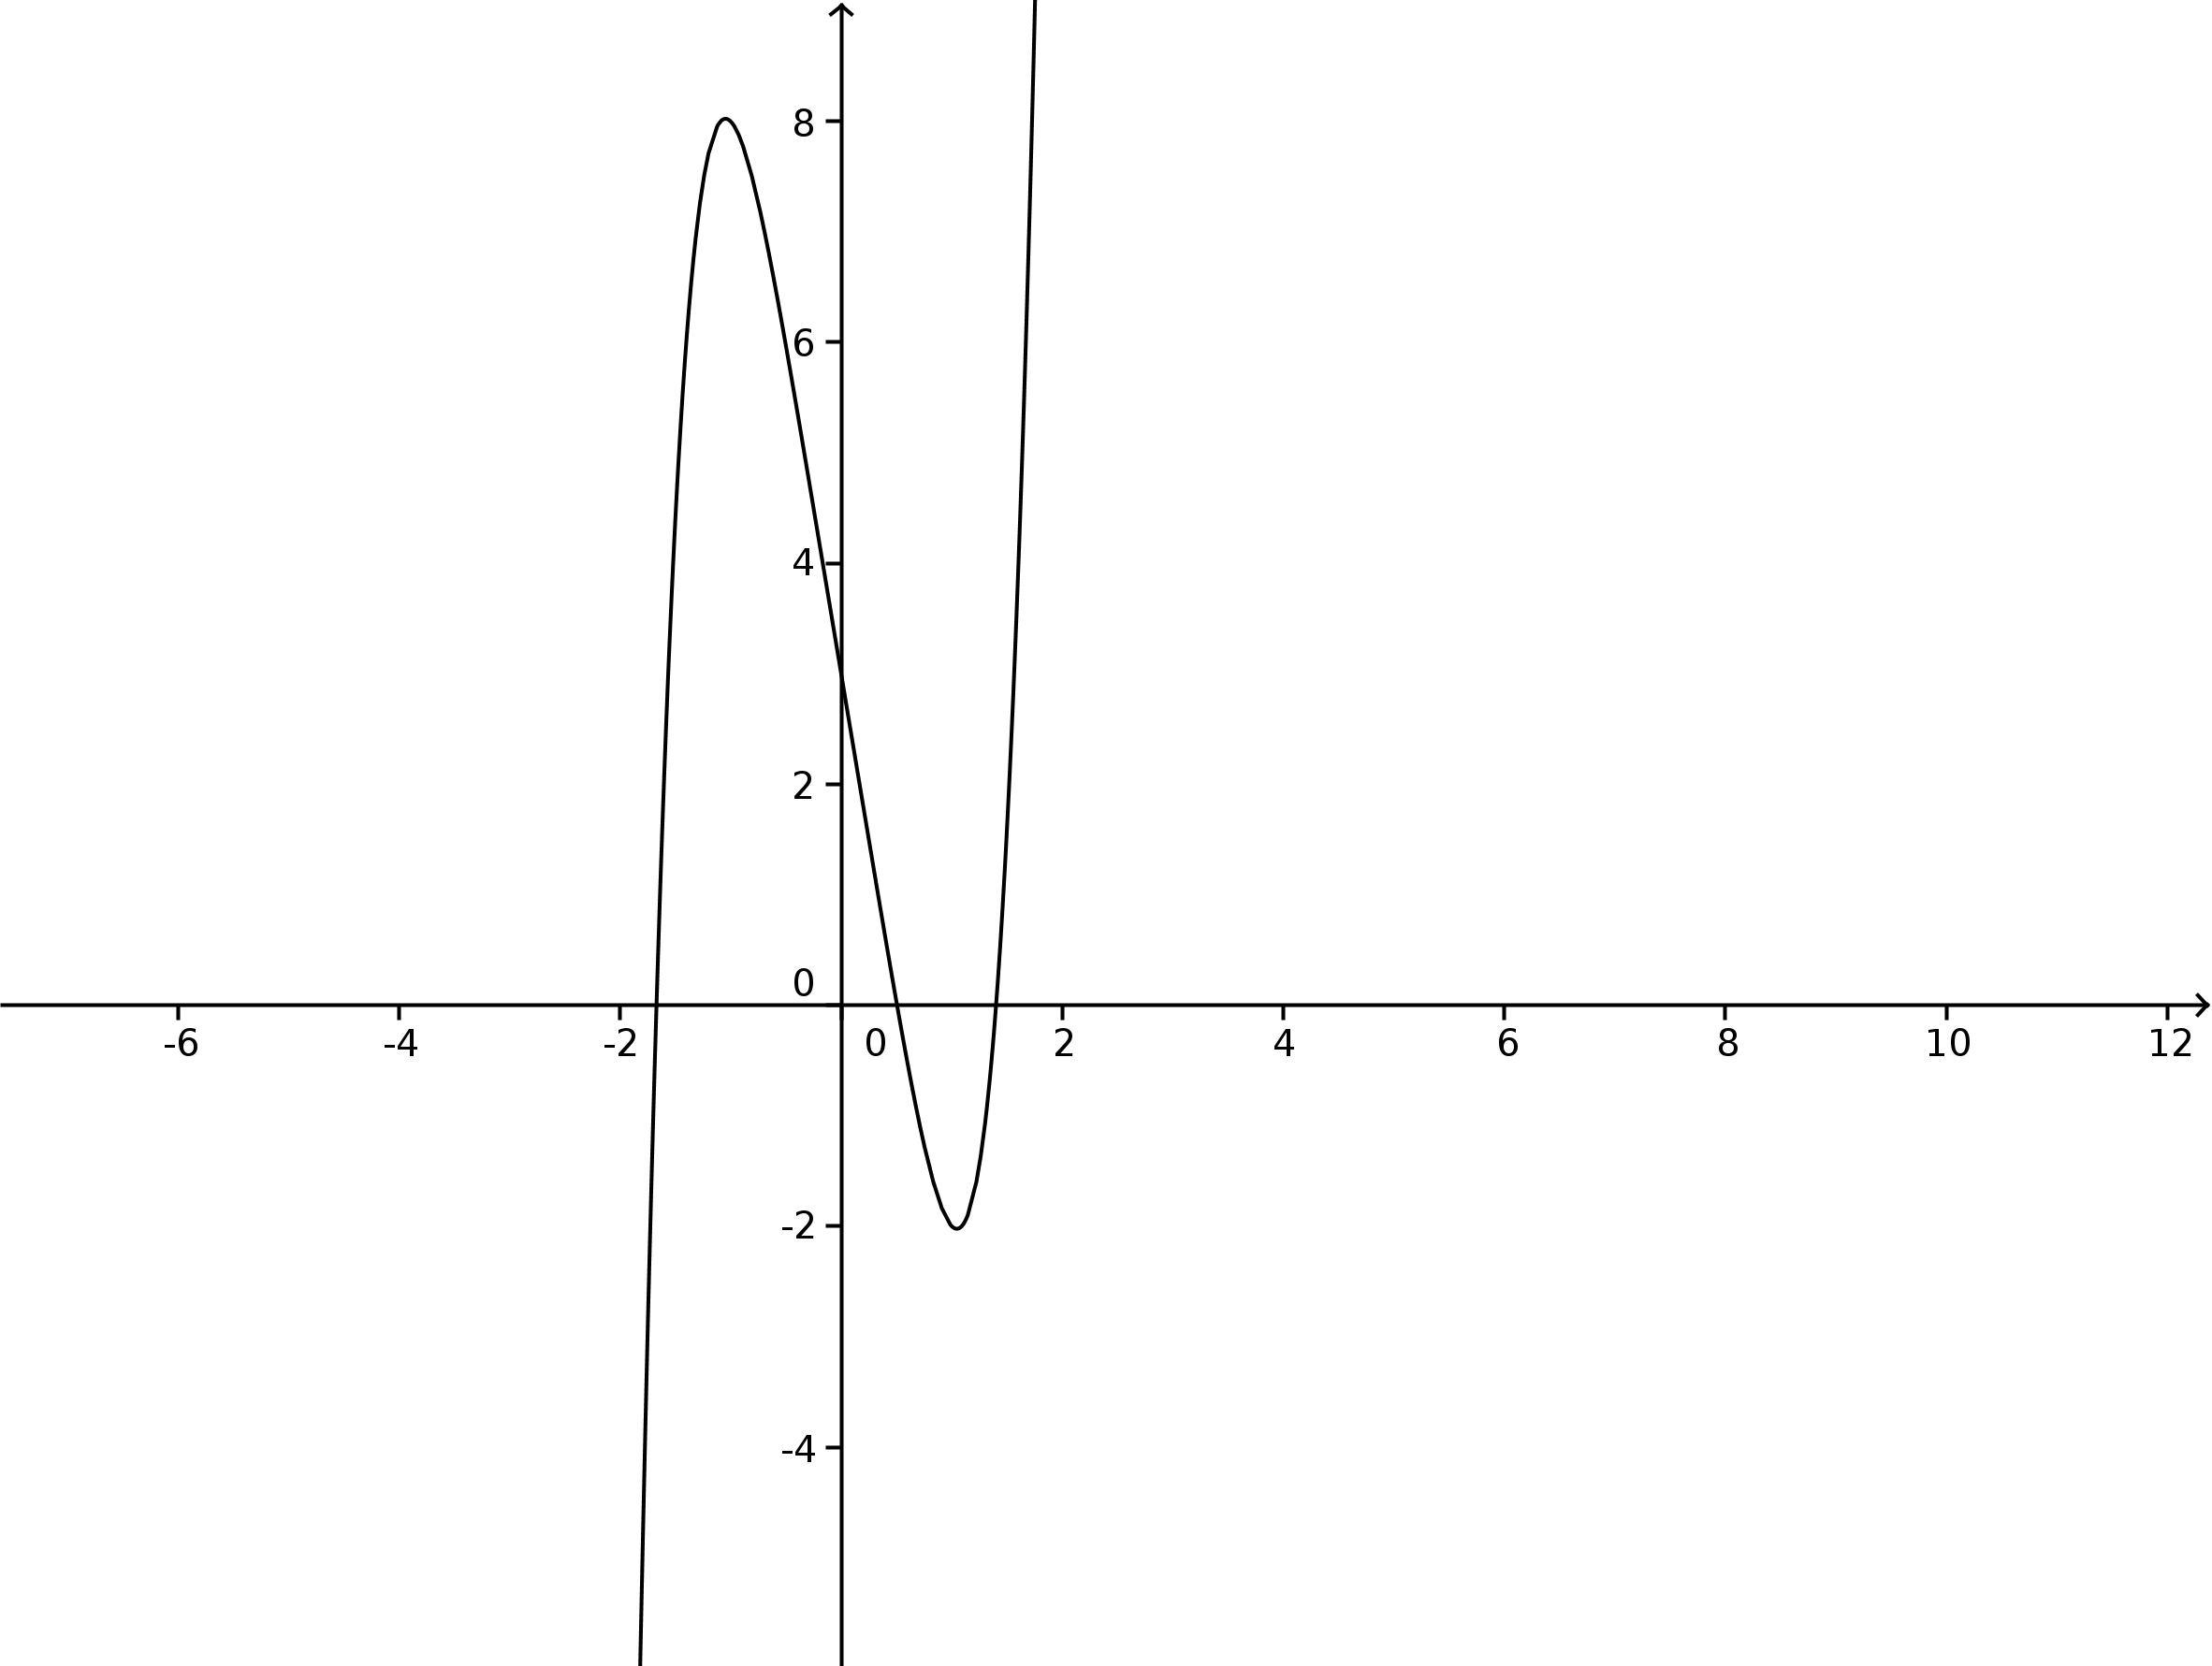
\includegraphics[scale=0.55]{img/polinomioIsoS5.png}\label{GrafPolIsoS5}


Viendo la gráfica (podríamos calcular la derivabilidad y ver cuando se anula y eso), vemos que hay 3 raíces reales ($x_3,x_4,x_5$) y 2 raíces complejas ($x_1,x_2$) conjugadas. Esta configuración de raíces del polinomio es la que asegura la isomorfidad a $S_5$, es decir,  cualquier polinomio con 3 raíces reales y 2 complejas conjugadas es irresoluble por radicales.
\end{proof}
Este ejemplo nos lleva a la siguiente proposición:


\begin{prop}[Irresolubilidad de grado 5]

Sea $f(t) ∈ℚ[t]$ irreducible (en $ℚ$) con dos raíces complejas (obviamente conjugadas) y 3 reales.

Sea $K$ su cuerpo de descomposición y $G = \gal(K/ℚ)$. \textbf{Entonces}
\[G\approx S_5\]

y por lo tanto $f(t) \text{ irresoluble por radicales}$.

\end{prop}
\begin{proof}
Vamos a ver que $G\approx S_5$, para demostrar la irresolubilidad.

Si tomamos $σ$ como la conjugación compleja $\implies σ$ induce un automorfismo de $K$, es decir $σ∈G=\gal(K/ℚ)$.

Podemos identificar $σ∈G$ con $s∈S_5$ de la siguiente manera $σ = (1,2)_{S_5}$, ya que $x_1,x_2∈ℂ \implies σ(x_1) = x_2, σ(x_2)=x_1$ y $x_3,x_4,x_5∈ℝ\implies  σ(x_i) = x_i, i=3,4,5$

Es decir, toma una inmersión de K en $\rac$ y conjuga el resultado haciendo que mande una raíz compleja en otra distina a la que lo hacía anteriormente y dejando el trabajo que la inmersión hacía sobre los reales fijo.


Ahora bien, $|G| = [K:ℚ] = 5d, \ d∈ℕ$, pues tenemos $ℚ\subset ℚ(x_1) \subset ℚ(x_1,x_2,x_3,x_4,x_5) = K$.

Por el teorema de Cauchy: %\ref{TmaCauchy}
$∃ τ ∈G, \ord(τ)=5$.

Recordamos que $S_5 = \gen{(1,2),(1,2,3,4,5)}$.

Ya lo tenemos demostrado, ya que $(σ∈G) \approx (1,2)∈S_5$ y por Cauchy sabemos que existe un elemento de grado 5 en $K$ identificable con $(1,2,3,4,5)$ (o una potencia suya), entonces $K = \gen{σ,τ} \approx \gen{(1,2),(1,2,3,4,5)}$, ya que tienen los mismos generadores.

\end{proof}




\appendix
\chapter{Resumen}

\section{Extensiones algebraicas}
\begin{itemize}
\item Dado $F$ subcuerpo de $E$ decimos que $E$ es una \textbf{extensión} de $F$ y la denotamos como $E/F$

\item Un elemento $α\in E$ es \textbf{algebraico} si existe un polinomio $p(x) \in F[x]$ que lo anula. Si todo elemento $α \in E$ es algebraico diremos que se trata de una \textbf{extensión algebraica}. Una extensión generada por elementos algebraicos es algebraica.

\item Podemos ver $E$ como un espacio vectorial sobre $F$. Diremos que $E$ es una \textbf{extensión finita} si es un espacio vectorial de dimensión finita sobre $F$.

Con [$E$:$F$] denotamos la dimensión de $E$ visto como espacio vectorial sobre $F$ y lo llamamos \textbf{grado de la extensión}

\item Si $E$ es una extensión finita sobre $F$ todo elemento de $E$ es algebraico. Es decir, toda extensión finita es algebraica.

\item Una extensión puede ser algebraica sin ser finita. Por ejemplo:
\[[\rac_{2^{\frac{1}{2}}, 2^{\frac{1}{3}}, ..., 2^{\frac{1}{n}}}:\rac] = \infty\]

\item Sea $α\in E$ algebraico sobre F y sea $n$ el grado de su polinomio mínimo irreducible sobre $F[t]$, entonces $F_{(α)}$ es una extensión de $F$ de grado $n$, generada por $1, α, α^2, ..., α^{n-1}$.

\item Dado un elemento α$\in E$ algebraico sobre $F$, $F_{(α)}$ es el mínimo cuerpo que contiene a $F$ y α. Por ser α algebraico, $F_{(α)}=F[α]$

\item $[E$:$F]$=1 $\iff$ $E=F$

\item Dadas las extensiones finitas $E_2$/$E_1$ y $E_1/F$, entonces:
\[[E_2:F]=[E_2:E_1]\times [E_1:F]\]

\item Un cuerpo es \textbf{algebraicamente cerrado} si todo polinomio de grado mayor o igual a 1 con coeficientes en él tiene una raiz dentro de ese mismo cuerpo. $\cplex$ es algebraicamente cerrado.Aplicando esta propiedad de forma recursiva vemos que en un cuerpo algebraicamente cerrado todo polinomio tiene tantas raíces en el cuerpo como grado tenga.

\item Dado un cuerpo $F$, llamamos \textbf{cierre algebraico} de $F$ al cuerpo $A$ que es algebraicamente cerrado y algebraico sobre $F$.

\item Definimos como \textbf{característica de un cuerpo} al número de veces que debemos sumar el neutro multiplicativo para obtener el neutro aditivo. Si no se puede obtener (por ejemplo, en $ℚ$ no podemos obtener el $0$ por muchas veces que sumemos $0$), se dice que el cuerpo tiene característica $1$.

\item Si $F$ es un subcuerpo de un cuerpo algebraicamente cerrado con característica 0, todo polinomio irreducible tiene tantas raices \textbf{distintas} como grado tenga.

\end{itemize}

\section{Inmersiones}
\begin{itemize}
\item Una \textbf{inmersión}, σ, es un homomorfismo que va de un cuerpo a otro. Siempre es inyectivo.

\item Sólo hay una inmersión de $\rac$ a cualquier cuerpo.

\item Si una inmersión es, además, sobreyectiva, será biyectiva y pasamos a denominarla \textbf{isomorfismo}

\item Dada una inmersión $\appl{σ}{F}{L}$, sea $p(t)$ un polinomio irreducible en $F[t]$, entonces $σ(p(t))$ es un polinomio irreducible en $L[t]$

\item Dada una inmersión $\appl{σ}{F}{L}$, si α es una raíz de $p(t) \in F[t]$, entonces σ(α) es una raíz en $σ(p(t))\in L[t]$

\item La imagen de un polinomio por una inmersión es el polinomio obtenido al aplicar la inmersión a los coeficientes.

\item Dada una inmersión $\appl{σ}{F}{L}$, sea $p(t)\in F[t]$ un polinomio irreducible y sea α una raíz del mismo en alguna extensión de $F$ y sea $\beta$ una raíz de $σ(f(t))$ en L, existe una inmersión $\appl{\tau}{F_{(α)}}{L}$ con $\tau(α) = \beta$

\item Sea $F$ un cuerpo y sea $p(t)\in F[t]$ un polinomio irreducible, entonces existe una extensión $E/F$ en la que $p(t)$ tiene una raíz.

\item Sea $E/F$ una extensión finita y sea $\appl{σ}{F}{A}$ una inmersión sobre un cuerpo algebraicamente cerrado. Entonces existe una extensión de σ a una inmersión $\appl{σ'}{E}{A}$

\item Sea α un elemento algebraico sobre $F$ y sea $p(t)$ su polinomio irreducible. Denotamos como $α_1,...α_n$ las raíces de $p(t)$ y las denominamos \textbf{conjugados de α sobre F}. Entonces para cada $α_i$ existe una inmersión que cumple $σ_i(α) = α_i$ y deja los elementos de $F$ como están.

\item Dada una extensión con $[E:F]=n$, sea $\appl{α}{F}{A}$ con $A$ algebraicamente cerrado con característica 0, entonces hay $n$ extensiones de $\sigma$ a inmersiones de $E$ en $A$.

\item Dado un cuerpo con característica 0, y dada una extensión del mismo $E/F$, existe un elemento $\gamma$ tal que $E=F_{(\gamma)}$. Un elemento como este $\gamma$ que nos permite generar toda una extensión se denomina \textbf{primitivo}

\item Las dos últimas proposiciones no se cumplen si el cuerpo $A$ no tiene característica 0. Con el fin de hacer algo similar en estos casos se añade una nueva condición.

Decimos que un polinomio $f(t)\in F[t]$ de grado $n$ es \textbf{separable} si tiene exactamente $n$ raíces distintas. Consecuentemente, un elemento $α\in E$ es \textbf{separable} (siendo $E$ una extensión de $F$) si su polinomio irreducible es separable. Decimos que una extensión finita es \textbf{separable} si el número de extensiones de una inmersión $\appl{α}{F}{A}$ a una inmersión de $E$ en $A$ es igual al grado $[E:F]$. (Siendo $A$ un cuerpo algebraicamente cerrado de característica arbitraria)

Estas son algunas propiedades sobre las extensiones separables que el libro pide demostrar:
\begin{itemize}
\item Si $E = F_{(α_1, α_2,...α_n)}$ y cada $α_i$ es separable sobre $F$, entonces $E$ es separable sobre $F$.
\item Si tenemos una torre de extensiones separables los límites de la torre constituyen una extensión separable.
\item Si $E$ es separable sobre $F$, todo subcuerpo de $E$ que contenga a $F$ será separable sobre $F$.
\item Sea $E$ una extensión finita separable de $F$, existe un elemento $\gamma$ tal que $E=F_{(\gamma)}$
\end{itemize}
\end{itemize}

\section{Cuerpos de descomposición}
\begin{itemize}
\item Sea $f(t) \in F[t]$ se dice que $E/F$ es el \textbf{cuerpo de descomposición} de $f(t)$ si podemos escribir $f(t)=(t-α_1)...(t-α_n) \in E[t]$ con $E=F_{(α_1,...α_n)}$. Es decir, añadimos al cuerpo las raíces del polinomio.

\item Para todo polinomio $f(t)\in F[t]$ existe un cuerpo de descomposición.

\item Si tenemos $K_1, K_2$ cuerpos de descomposición de un mismo polinomio $f(t) \in F[t]$, entonces existe un isomorfismo que extiende la identidad en $F$ y que va de $K_1$ a $K_2$..

\item Una extensión se llama \textbf{normal} si es el cuerpo de descomposición de algún poliniomio $f(t) \in F[t]$.

\item Sea $K$ una extensión normal de $F$. Si $p(t) \in F[t]$ es irreducible sobre $F[t]$ y tiene una raíz en $K$, entonces $p(t)$ tiene todas sus raíces en $K$.
\end{itemize}

\section{Teoría de Galois}
\begin{itemize}

\item Una extensión es \textbf{galoisiana} si es normal y separable. En característica 0 toda extensión normal será una extensión galoisiana.

\item A partir de una extensión galoisiona podemos definir el \textbf{grupo de Galois} como:
\[Gal(E/F) = \left\{\appl{σ}{E}{E} \text{ automorfismo} \tq σ_{|F} = id\right\}\]
Además, $\#(Gal(E/F))=[E:F]$.

\item \textbf{Teorema fundamental de la teoría de Galois}. Sea $K/F$ una extensión galoisiana y finta:
\begin{enumerate}
\item Se tiene la biyección:
\[\{E | F\subset E \subset K\} \rightarrow \text{subgrupos de }Gal(K/F)\]
tal que:
\[E \rightarrow Gal(K/E)\]
\[K^H=\{x \in K | \sigma(x)=x \forall \sigma \in H\}\leftarrow H\]
\item $\forall H < G$, la extensión $K/K^H$ es galoisiana y $[K:K^H]=\abs{H}$
\item $[K^H:F]=\frac{|G|}{|H|}=\frac{[K:F]}{|H|}$
\item $K^H/F$ es galois $\iff H \lhd G$ y además:
\[G/H \longrightarrow Gal(K^H/F)\]
		\[σ \longmapsto σ_{|K^H}\]
\end{enumerate}

\end{itemize}


\chapter{Ejercicios}

% -*- root: ../TeoriaGalois.tex -*-
\section{Hoja 1}

\begin{problem} Encuentra el grado de las siguientes extensiones.
\solution
\begin{enumerate}
\item $[ℚ(\sqrt{2}) : ℚ ]= 2$.
\item $[ℚ(\sqrt{6}) : ℚ ]= 2$ con $p(t) = t^2 - 6$: su solución es $\sqrt{6}$ que no está en $ℚ$. El criterio de Eisenstein también funciona con $p=2$: $p$ divide al término independiente pero no al de mayor grado.
\item $[ℚ(\sqrt{16}) : ℚ ]= 1$ con $p(t) = t-4$.
\item $[ℚ(\sqrt{p}) : ℚ] = 2$ con $p$ primo, siendo $p(t) = t^2 - p$.
\item $[ℚ\left(e^{\frac{2πi}{n}}\right) : ℚ]$ con $n=2,3,4,5,6,8$.
\begin{enumerate}
\item Para $n=2$, $e^{\frac{2πi}{n}} = -1$ y $[ℚ(-1):ℚ] =  1$.

\item Para $n=3$, el polinomio que lo anula es $p(t) = t^3 - 1$, pero no es irreducible porque tiene como raíz $1$, y entonces $p(t) = (t-1) (t^2 + t + 1)$. Luego $e^{\frac{2πi}{3}}$ es raíz de $t^2+t+1$, que tiene que ser irreducible (si una raíz,$e^{\frac{2πi}{n}}$, es compleja, la otra es su conjugado, que también es complejo). $[ℚ\left(e^{\frac{2πi}{3}}\right) : ℚ] = 2$.

\item Para $n=4$, $e^{\frac{2πi}{4}} = i$, luego $[ℚ(i) : ℚ ] = 2$ con $p(t) = t^2 + 1$. Si no fuese $p(t)$ irreducible, tendríamos de nuevo que $[ℚ(i) : ℚ]=1$ y $ℚ(i)$ sería igual a $ℚ$, lo cual es absurdo porque $i$ no está en $ℚ$.

\item Para $n=5$, está claro que $h(t) = t^5 - 1$ anula a $e^{\frac{2πi}{5}}$, luego el grado de la extensión es menor o igual que 5. Desde luego no es irreducible porque 1 es raíz $h(t) = (t-1)(t^4 + t^3 + t^2 + t + 1)$. $e^{\frac{2πi}{5}}$ debe ser raíz de $t^4 + t^3 + t^2 + t + 1$. ¿Es este polinomio irreducible? Desarrollaremos un método más general para encontrar los polinomios irreducibles de las raíces de la unidad, pero para este nos quedamos con una sugerencia: sí es irreducible y $[ℚ\left(e^{\frac{2πi}{5}}\right): ℚ ] = 4$. Sólo hay que estudiar la aplicación $ℚ[t] \mapsto ℚ[t]$ que manda $t$ a $t+1$ y por lo tanto $\sum a_i t^i \mapsto \sum a_i (t+1)^i$, que si es un isomorfismo de anillos entonces $p(t)$ es irreducible si y sólo si $p(t+1)$ lo es. En este caso podríamos usar el criterio de Eisenstein para probarlo. Esto se resolvi\'o en un ejemplo de teor\'ia (\ref{Teoria_H1.E1.A5.S_Af})

\item Para $n=6$, $h(t) = t^6 - 1$ lo anula, pero podemos descomponerlo como $h(t) = (t^3 - 1)(t^3 + 1)$. $e^{\frac{2πi}{6}}$ es raíz sólo de $t^3 + 1$, pero este polinomio tampoco es irreducible: $t^3 + 1 = (t-1)(t^2 - t + 1)$. $e^{\frac{2πi}{6}}$ es raíz de $t^2-t+1$, que por el mismo argumento que en el caso $n=4$ tiene que ser irreducible, o si no un número complejo estaría en $ℚ$.

\item Por último, cuando $n=8$, sabemos que $h(t) = t^8 - 1$ anula a $e^{\frac{2πi}{8}}$. Pero descomponiendo de nuevo, $h(t) = (t^4 -1)(t^4 +1)$, $e^{\frac{2πi}{8}}$ es raíz de $t^4 +1$, el grado de la extensión es menor o igual que cuatro. Por suerte, $t^4 + 1$ es irreducible: las raíces deberían ser enteras y dividir a $1$, y ni $1$ ni $-1$ son raíces.
\end{enumerate}
\end{enumerate}
\end{problem}


\begin{problem}Encuentra el grado de las siguientes extensiones

\solution

\begin{itemize}

\item $[\rac(\sqrt{6},i):\rac]$.

 Para resolver estos ejercicios, el procedimiento es escribirlo desmenuzadas las inclusiones.

$\rac \to \rac(\sqrt{6}) \to \rac(\sqrt{6})(i) = \rac(\sqrt{6},i)$

Y vamos caso por caso:

\begin{itemize}
\item $[\rac: \rac(\sqrt{6})] = 2$
\item $[\rac(i): \rac(\sqrt{6}) ] = 2 (i \notin \rac(\sqrt{6}))$
\end{itemize}

Entonces: $[\rac(\sqrt{6},i):\rac]= 2\cdot 2 = 4$.

\item $[\rac(\sqrt[n]{p},\sqrt{-m}):\rac] = 2n$. Se resuelve generalizando la misma idea del anterior.

\item $[ℚ(\sqrt[3]{2},e^{\frac{2 \pi i}{3}}\cdot \sqrt[3]{2}):ℚ]$

Lo primero que nos tenemos que dar cuenta es de que \\
 $ℚ(\sqrt[3]{2},e^{\frac{2 \pi i}{3}}\cdot \sqrt[3]{2}) = ℚ(\sqrt[3]{2},e^{\frac{2 \pi i}{3}})$

Ahora escribimos la cadena de inclusiones:

\begin{gather*}
[ℚ : ℚ(\sqrt[3]{2})] = 3, p(t)=t³-2\\
[ℚ(\sqrt[3]{2}) : ℚ(\sqrt[3]{2})(e^{\frac{2\pi i}{3}})]  [ℚ(e^{\frac{2\pi i}{3}})] = 2; p(t) =  t²+t+1\\
[ℚ(\sqrt[3]{2}) : ℚ(\sqrt[3]{2})(e^{\frac{2\pi i}{3}})] = 2; e^{\frac{2\pi i}{3}}∉ℚ(\sqrt[3]{2})
\end{gather*}

Entonces deducimos que $[ℚ(\sqrt[3]{2},e^{\frac{2 \pi i}{3}}\cdot \sqrt[3]{2}):ℚ] = 2·3 = 6$
\end{itemize}

\end{problem}


\begin{problem}[3]
Sean $E₁$ y $E₂$ dos extensiones distintas de un cuerpo $F$ de grados $p$ y $p'$ respectivamente, donde $p$ y $p'$ son
primos distintos. Demostrar que $E_1 ∩ E_2 = F$.

\solution

Está claro que $E_1 ∩ E_2 ⊆ E_1$, así que podemos considerar la cadena de extensiones \[ E_1 \hookrightarrow E_1 ∩ E_2 \hookrightarrow F \]

Entonces, $p = [E_1 : F] = [E_1 : E_1 ∩ E_2] · [E_1 ∩ E_2 : F]$. Como $p$ es primo, sólo puede ser $E_1 = E_1 ∩ E_2$ o bien $E_1 ∩ E_2 = F$. Lo primero no puede ocurrir: si $E_1 ∩ E_2 = E_1$ entonces $E_1 ⊆ E_2$, así que tendríamos $[E_2:F] = p' = [E_2 : E_1] · [E_1 : F]$, imposible porque $p'$ es primo.

\end{problem}

\begin{problem}[4]
Sea $K$ un cuerpo finito. Demostrar que $\card{K} = p^m$ para algún primo $p$.

Demuestra que además, ese $p$ es la característica $\mop{char}(K)$ de $K$.
\solution

Lo primero es recordar la \concept[Característica]{característica}: el número de veces que tienes que sumar la unidad para llegar al 0 en cuerpos finitos.

Por ser $K$ un cuerpo finito, podemos definir el siguiente homomorfismo φ de anillos que nos lleve de $ℤ$ al cuerpo $K$:

\begin{align*}
ℤ &\longmapsto K \\
1 &\longmapsto 1_K \\
α &\longmapsto α·1_K = 1_K + \dotsb + 1_K
\end{align*}

Estudiemos el núcleo de φ. Son los elementos de $ℤ$ cuya imagen es la unidad en $K$, esto es, tomando $n = \mop{char}(K)$, \[ \ker φ = \set{a·n \tq a ∈ ℤ} = nℤ \]

El segundo teorema de isomorfía de grupos\footnote{Ver magníficos apuntes de Pedro Valero de Estructuras Algebraicas.} nos dice que existe un isomorfismo entre la imagen de $φ$ y el grupo cociente $\quot{ℤ}{\ker φ}$, al que llamaremos $γ$:

\[ \appl{γ}{\quot{ℤ}{nℤ} = \fd_n}{\img φ ⊆ K} \]

Afirmamos que $n≠0$: $K$ es finito y $\quot{ℤ}{0ℤ} = ℤ$, así que no puede existir un isomorfismo entre ambos.

Afirmamos que $n$ es primo, y vamos a demostrarlo por reducción al absurdo. Supongamos $n = ab$. Si operamos en $\fd_n$, tenemos que $n\equiv 0 \mod n$ y entonces $ab=0$. Aplicamos $γ$ a ambos lados y tendríamos que $γ(a)·γ(b) = γ(0) = 0_K$, contradicción ($K$ es un cuerpo así que no puede tener divisores de $0$).

Sea $p=n$, entonces \[ \mathbb{F}_p = \quot{ℤ}{nℤ}  \simeq \img φ \] es un subcuerpo de $K$, luego $K$ es un espacio vectorial sobre $\mathbb{F}_p$. Es decir, que si $[K:\mathbb{F}_p] = m$, entonces $\{x₁, \dotsc, x_m\}$ es base de $K$ sobre $\mathbb{F}_p$, luego \[ \card{K} = \card{\fd_p}^{[K:\fd_p]} = p^m\] para $m ≥ 1$, y ya tenemos lo que buscábamos.

Una observación importante: el cuerpo finito de $n$ elementos \textbf{no es} $\quot{ℤ}{nℤ}$. Los enteros módulo $n$ sólo son un cuerpo cuando $n$ es primo. Es decir, que en general \[ \fd_n ≠ \quot{ℤ}{nℤ} \].

Los cuerpos finitos hay que construirlos específicamente como el cociente de un cuerpo finito de orden primo con el ideal generado por un polinomio irreducile. Por ejemplo, podríamos preguntarnos si hay un cuerpo con 9 elementos. Existe, porque $9=3^2$.

El problema 4 de la hoja 2 (que incluye al 6 de la hoja 1) va precisamente de construir este cuerpo.
\end{problem}


%%%%%%%%%% Malvado 2-10-2014 %%%%%%%%%%%%%
\section{Hoja 2}

% Ejercicio 1
\begin{problem}[1] Inmersiones de $ℚ(\alpha)$ en $ℂ$
\solution
\begin{enumerate}
	\item $\alpha \eq \sqrt{2}$.\\
	{\inputtikz{ejercicios/img1-ej1-h2}} \\
	$\sigma(\sqrt{2}) \eq \sqrt{2}  \Rightarrow \sigma_1 \eq Id$ \\
	$\sigma_2(\sqrt{2}) \eq -\sqrt{2}$

	\item $\alpha \eq i \eq \sqrt{2}$ \\
	{\inputtikz{ejercicios/img2-ej1-h2}} \\
	$p(t) = t^2 + 1$\\
	$\sigma_1(i) \eq i \Rightarrow \sigma_1 \eq Id$\\
	$\sigma_2(i) \eq -i \Rightarrow \sigma_2 \eq$ conjugación compleja\\
	$\sigma_2(a+bi) \eq a + b(-i) = a + bi$

	\item $\alpha \eq \sqrt[3]{2}$\\
	{\inputtikz{ejercicios/img3-ej1-h2}} \\
	polinomio mínimo de $\sqrt[3]{2}$ es $p(t) \eq t^3 - 2$\\
	raíces $\sqrt[3]{2}, e^{\frac{2πi}{3}}\sqrt[3]{2}, e^{\frac{4πi}{3}}\sqrt[3]{2}$\\
	$\sigma_1(\sqrt[3]{2}) \eq \sqrt[3]{2} \implies \sigma_1 \eq Id$\\
	$\sigma_2(\sqrt[3]{2}) \eq e^{\frac{2πi}{3}}\sqrt[3]{2}$\\
	$\sigma_3(\sqrt[3]{2}) \eq e^{\frac{4πi}{3}}\sqrt[3]{2}$

	E.G $x \eq 7 + 2\sqrt[3]{2} + 5(\sqrt[3]{2})^2 \in ℚ(\sqrt[3]{2})$\\
	$\sigma_2(x) = 7 + 2e^{\frac{2πi}{3}}\sqrt[3]{2} + 5e^{\frac{4πi}{3}}(\sqrt[3]{2})^2$

	¿Cuáles son entonces?
	$\sigma_2(ℚ(\sqrt[3]{2})) \eq ℚ(e^{\frac{2πi}{3}}\sqrt[3]{2}) \neq ℚ(\sqrt[3]{2})$ con $\sigma_2(ℚ(\sqrt[3]{2})) \subset \real$
\end{enumerate}
\end{problem}


% Ejercicio 2
\begin{problem}[2]

\ppart Escribir todos los automorfismos de $ℚ(e^{\frac{2πi}{8}})$ que extienden el automorfismo $\sigma: ℚ(i) \rightarrow ℚ(i)$ que envía $i$ a $-i$.

\ppart Escribir todos los automorfismos de $ℚ(e^{\frac{2πi}{8}})$.

\solution

\spart

\begin{wrapfigure}{R}{0.4\textwidth}
\centering
\inputtikz{ejercicios/img1-ej2-h2}
\caption{Esquema de las inmersiones que buscamos, con $σ$ tal que $σ(i) = -i$.}
\end{wrapfigure}

Lo primero que buscamos es el polinomio irreducible de $e^{\frac{2πi}{8}}$ sobre $ℚ(i)$. Vemos que \[ (t^4 + 1)(t^4 - 1) = t^8 - 1 \] anula a $e^{\frac{2πi}{8}}$.

$t^4 + 1$ era el polinomio irreducible de $e^{\frac{2πi}{8}}$ sobre $ℚ$; y como sobre $ℚ(i)$ $t^4 + 1 \eq (t^2 - i)(t^2 + i)$, el polinomio irreducible de $e^{\frac{2πi}{8}}$ sobre $ℚ(i)$ es $p(t) = t^2 - i$, pues \[ \left(e^{\frac{2πi}{8}}\right)^2 \eq
e^{\frac{πi}{2}} \eq i \]

El polinomio mínimo es de grado dos, así que tenemos que encontrar dos extensiones, que serán

\begin{align*}
	\sigma_1(e^{\frac{2πi}{8}}) &\eq w_1 \neq e^{\frac{2πi}{8}} \\
	\sigma_2(e^{\frac{2πi}{8}}) &\eq w_2 \neq e^{\frac{2πi}{8}} \\
\end{align*}
donde $w_1$ y $w_2$ son raíces de $p^{\sigma}(t) \eq t^2 + i$.

\spart

\begin{wrapfigure}{R}{0.4\textwidth}
\centering
\begin{tabular}{r|c|c}
$\;$  & $i$ & α 	\\ \hline
$σ_1$ & $i$ & $α$  	\\
$σ_2$ & $i$ & $-α$  \\ \hline
$σ_3$ & $-i$ & $α$ 	\\
$σ_4$ & $-i$ & $-α$	\\
\end{tabular}
\caption{Automorfismos de $ℚ(α)$.}
\label{tblH2E2}
\end{wrapfigure}

Los automorfismos deben dejar fijos los elementos de $ℚ$ y llevar raíces del polinomio mínimo de $e^{\frac{2πi}{8}} = α$ a otras raíces del mismo polinomio. En el apartado anterior habíamos visto que este polinomio era $t^4 + 1 = (t^2 - i)(t^2 + i)$, así que los automorfismos se caracterizarán por la imagen de $i$ y $α$. Los tenemos definidos en la tabla lateral \ref{tblH2E2}.

\end{problem}

\begin{problem}[3] Encontrar todas las inmersionces de $ℚ(α,β)$ en $ℚ$ donde

\ppart $α=\sqrt{2},\; β=\sqrt{3}$.
\ppart $α = \sqrt{6},\; β = i = \sqrt{-1}$.
\ppart $α = \sqrt[3]{2},\; β = i$.

\solution

\spart
\spart
\spart

\begin{wrapfigure}{R}{0.4\textwidth}
\centering
\begin{tabular}{r|c|c}
$\;$  & $i$ & α \\\hline
$σ_1$ & $i$ &  $α$  \\
$σ_2$ & $i$ & $ω_3α$  \\
$σ_3$ & $i$ & $ω_3^2α$\\\hline
$σ_4$ & $.i$ & $α$ \\
$σ_5$ & $-i$ & $ωα$\\
$σ_6$ & $-i$ & $ω^2α$
\end{tabular}
\caption{Tabla de inmersiones de $ℚ\left(\sqrt[3]{2}, i\right)$ en $ℚ$.}
\label{tblH2E3}
\end{wrapfigure}

Es fácil de comprobar que \[ [ℚ(\sqrt[3]{2},i):ℚ] = 6 \]

Ahora vamos a añadirle algo de complejidad/interés al problema calculando el elemento primitivo de esta extensión.

Un elemento primitivo de $ℚ(\sqrt[3]{2},i) / ℚ$ sería $γ = i + \sqrt[3]{2}$.
Con el fin de simplificar la notación representaremos $ω=\sqrt[3]{2}$
Tenemos varias maneras de comprobar que el elemento es primitivo, podemos utilizar el algoritmo de ir elevando a potencias y acabar calculando el polinomio irreducile y ver su grado, o escribir todas las inmersiones que es lo que vamos a utilizar (tabla \ref{tblH2E3}). Lo mismo hicimos en \ref{tblGaloisT4-2}.

(Donde $ω$ serían números complejos que nos permiten obtener el resto de raíces del polinomio irreducible de α)

Ahora comprobamos que $σ_k (γ) ≠ σ_l(γ) \dimplies k≠l\; k,l=1,\dotsc,6$.

\end{problem}

\paragraph{Interesante:}

Las extensiones no tienen polinomios. Las extensiones tienen elementos y son éstos los que tienen polinomios.  Si ese elemento es primitivo, el grado del polinomio del elemento será el grado de la extensión.

%Ejercicio 4
\begin{problem}[4]
 \label{H1.E6}
 Construir un cuerpo con 9 elementos (como un cociente adecuado del anillo de polinomios $\mathbb{F}_3 [x]$ ).

\solution

Como veíamos en el ejercicio 4 de la hoja 1, como $9=3^2$, entonces existe un cuerpo $K$ de nueve elementos que contiene a $\fd_3$.

Sabemos que $\quot{\mathbb{F}_3[t]}{(p(t))}$ es un cuerpo si $p(t) \in \mathbb{F}_3[t]$ es irreducible. Además, es una extensión de grado $\deg p(t)$ sobre $\fd_3$.

Por lo tanto, necesitamos un polinomio $p(t)$ con $\deg p(t) = 2$ para que $\card{K} = 3^2 = 9$.

Tomemos por ejemplo $p(t) = 1+t+t^2 ∈ \mathbb{F}_3$. ¿Este polinomio es irreducible? no, porque 1 es raíz: $\overline{1}+\overline{1}+\overline{1}^2 = \overline{3} = \overline{0}$.

Vamos a buscar otro: sea $p(t) = 1+t^2$. Esta vez sí es irreducible: operando con los tres elementos de $\fd_3$ tenemos que $p(0) = 1,\, p(1) = 2,\, p(2) = 2$, ninguno es raíz.

Entonces \[ K = \quot{\mathbb{F}_3[t]}{(t^2+1)} \] es un cuerpo por ser $p(t)$ irreducible. \footnote{Igual que $\displaystyle\quot{ℝ}{(x^2+1)} = ℂ$ es un cuerpo, por ejemplo}

Sea entonces $α$ un símbolo con la propiedad $α^2 = -1$. Su polinomio mínimo sobre $\fd_3[t]$ es $p(t) = t^2 + 1$. Como el grado de este polinomio es dos, el grado de la extensión $[\fd_3(α) : \fd_3]$ será $2$, luego $\card{\fd_3 (α)} = 3^2 = 9$, el cuerpo que buscábamos.

¿Cómo es $K$? Es un anillo cociente, luego es el conjunto de todas las clases de equivalencia \[ [f(t)] = \set{f(t) + g(t) · p(t) \tq g(t) ∈ \fd_3[t]}\] con $f(t) ∈ \fd_3[t]$. Dicho de otra forma, igual que considerábamos la clase de equivalencia de $a$ en $ℤ_n$ como todos los enteros cuyo resto al ser divididos por $n$ es $a$, aquí la clase de equivalencia de $f(t)$ son todos los polinomios con coeficientes en $\fd_3$ cuyo resto al dividir por $p(t)$ es $f(t)$.

Podemos simplificar la construcción anterior para hacerla más manejable. Como $p(α) = 0$, las clases de equivalencia se caracterizan por su resto al dividirlas por $p(t)$, ya que tenemos que $f(α) + g(α) · p(α) = f(α) \; ∀g(t) ∈ \fd_3[t]$.

Así, podemos decir que los elementos de $K$ son los restos de dividir polinomios de $\fd_3 [t]$ entre $p(t)$. Es decir, serán elementos de la forma \[ x = a + b α\] con $a,b ∈ \fd_3$. Precisamente así es muy fácil ver que, como podemos escoger $a$ y $b$ de tres formas distintas cada uno, tenemos en total $3^2 = 9$ elementos.
\end{problem}

\section{Hoja 3}

\begin{problem}[1] Encontrar un elemento primitivo y su correspondiente polinomio irreducible de la extensión $\quot{ℚ(α,β)}{ℚ}$ donde
\ppart $α = \sqrt{2},\; β = i$.
\ppart $α = \sqrt{2},\; β = \sqrt{3}$.
\ppart $α = \sqrt{2},\; β = 7 + \sqrt{2}$.
\solution

\spart

El elemento primitivo puede ser $\sqrt{2} + i$, ya que podemos operar y ver que obtenemos $\sqrt{2}$ e $i$ (ejemplo de esto en la definición de elemento primitivo, \ref{DefElemPrimitivo}). Su polinomio mínimo será \[ p(t) = 9 - 2t^2 + t^4\]

\spart

Este vamos a hacerlo completo. Supongamos que el elemento primitivo es $γ = \sqrt{2} + \sqrt{3} = α + β$. Primero tenemos que ver que $ℚ(γ) = ℚ(α,β)$, y para esto tenemos que ver que $α, β ∈ ℚ(γ)$. Empezamos obteniendo las potencias de $γ$, que nos servirán más tarde para el polinomio mínimo:

\begin{align*}
γ &= α + β \\
γ^2 &= 5 + 2αβ \\
γ^3 &= 11α + 9β \\
γ^4 &= 49 + 20αβ
\end{align*}

Si operamos, tenemos que $γ^3 - 9γ = 2α$. Como $2∈ℚ$, tiene que ser $α ∈ ℚ(γ)$, y con esto podemos sacar que $β ∈ ℚ(γ)$.

Ahora falta ver el polinomio mínimo. Buscamos $p(t) ∈ ℚ[t]$ tal que $p(γ) = 0$, esto es \[ 0 = a γ^4 + b γ^3 + c γ^2 + d γ + e \]

Si sustituimos las potencias que hemos calculado antes y agrupamos por los elementos de la base de $ℚ(γ)$ (es decir, $\set{1, α, β, αβ}$) tenemos que

\begin{align*}
0 &= a 49 + a20αβ + b11α + b9β + c5 + c2αb + dα + dβ + e = \\
&= (e + 49a + 5c)·1 + (11b + d)·α + (9b + d)·β + (20a + 2c) ·αβ = 0
\end{align*}

Cada uno de los factores tiene que ser cero, así que resolvemos el sistema

\begin{align*}
0 &= 49a + 5c + e \\
0 &= 11b + d \\
0 &= 9b + d \\
0 &= 20a + 2c
\end{align*}

De la segunda y tercera ecuaciones sacamos que $b = d = 0$. De la última, que $c = -10a$, y sustituyendo con esto en la primera, que $e = a$. Como buscamos que $p(t)$ sea mónico, tomamos $a = 1$ y entonces nos queda

\[ p(t) = t^4 - 10t^2 + 1 \]

\spart

Dado que $ℚ(\sqrt{2}) = ℚ(7 + \sqrt{2})$ al estar $7 ∈ ℚ$, el elemento primitivo es $\sqrt{2}$ con polinomio mínimo $p(t) = t^2 - 2$.
\end{problem}

\begin{problem}[3]

\ppart Calcular el grado de la extensión $\mathbb{F}_3(x, y)/\mathbb{F}_3(x^3, y^3)$.

\ppart Encontrar todas la extensiones de la inclusión $\mathbb{F}_3 (x^3 , y^3) \hookrightarrow \mathbb{F}_3(x, y)$.

\ppart Probar que esta extensión no tiene elementos primitivos.

\solution

Pequeño anexo interesante: $\mathbb{F}_9 ≠ ℤ_9$, $\frac{\mathbb{F}_3[x]}{x^2+1}$

\spart Calculamos el grado de la extensión a partir de la siguiente cadena de inclusiones

\[
\begin{array}{ccccc}
\mathbb{F}_3(x^3,y^3) & \hookrightarrow
	& \mathbb{F}_3(x^3,y^3)(x) & \hookrightarrow
	& \mathbb{F}_3(x,y^3)(y) \\
& \downarrow & & \downarrow & \\
& p_1(t) = t^3-x^3 & & p_2(t) = t^3-y^3 &
\end{array}
\]

$p_1$, $p_2$ serán irreducibles sii no tienen raíces en $\mathbb{F}_3(x^3,y^3)$, y en ese caso tendremos que $[\fd_3(x,y): \fd_3(x^3,y^3)] = 9$.

Esto es sencillo de comprobar puesto que sabemos que $t^3-x^3 = (t-x)^3$ en $\mathbb{F}_3(x,y)$, y este polinomio solo tiene una raíz, que es $x$.

Ahora la única posibilidad de que no fuese irreducible es que resulte que $x\in \mathbb{F}_3(x^3,y^3)$. En ese caso resultaría que la extensión tendría grado 1 pues estaríamos 'añadiendo' un elemento que ya está en el cuerpo.

Si $x$ perteneciera a $\mathbb{F}_3(x^3,y^3)$, entonces podríamos escribir:
\[x = \frac{\sum a_{ij}(x^3)^i(y^3)^j}{\sum b_{ij}(x^3)^i(y^3)^j}; \quad a_{ij},b_{ij} ∈ \mathbb{F}_3\] que es equivalente a que
\[ \sum b_{ij} x^{3i+1}y^{3j} = \sum a_{ij} x^{3i}y^{3j}\]

Para que estos dos polinomios sean iguales debemos igualar sus coeficientes uno a uno. Para cada $j$ el coeficiente de $y^{3j}$ debería ser igual a un lado y al otro de la igualdad, es decir:
\[b_{ij}x^{3i+1}=a_{ij}x^{3i}\]

Y vemos fácilmente que para $i$ que fijemos no existen unas constantes $a,b$ que satisfagan la ecuación.

\spart Esto es paradigmático. Este es un buen ejemplo de algo que veremos más adelante.

En la cadena:
$$\begin{array}{ccccc}\mathbb{F}_3(x^3,y^3) &\subset& \mathbb{F}_3(x^3,y^3)(x) &\subset& \mathbb{F}_3(x,y^3)(y)\\
\end{array}$$

las únicas extensiones posibles en ambas inclusiones son la identidad, ya que por fuerza, $σ(x) = x$ porque $σ$ manda raíces de polinomios en raíces de polinomios.

Podemos concluir que esta extensión es normal, pero no es separable. Se deja como ejercicio para el lector la comprobación de estas afirmaciones.

\spart Se trata de un ejercicio de examen salvo por un pequeño detalle, y es que en el examen daban una pista extra:
\[γ∈\mathbb{F}_3(x,y) \implies γ^3 ∈\mathbb{F}_3(x^3,y^3)\]

Supongamos que esto es verdad. Entonces:

\[[\mathbb{F}_3(x^3,y^3)(γ) : \mathbb{F}_3(x^3,y^3)] ≤ 3\]

porque $γ$ satisface el polinomio $t^3 -γ^3 ∈ \mathbb{F}_3(x^3,y^3)[t]$

\[γ = \frac{\sum a_{ij}(x^3)^i(y^3)^j}{\sum b_{ij}(x^3)^i(y^3)^j}; a_{ij},b_{ij} ∈ \mathbb{F}_3\]

Vamos a demostrar la pista que, en el examen, nos daba el enunciado.

Para ello, fjémonos en el valor de $γ^3$. Como el cuerpo en el que nos movemos tiene $Ch(\mathbb{F}) = 3$ se cumple que $(a+b)^{3} = a^3 + b^3$.

Por tanto:
\[γ^3 = \frac{\sum a_{ij}^3(x^3)^i(y^3)^i}{\sum b_{ij}^3(x^3)^i(y^3)^i}; a_{ij},b_{ij} ∈ \mathbb{F}_3 \implies γ^3 ∈ \mathbb{F}_3 \implies [\mathbb{F}_3(x^3,y^3)(γ) : \mathbb{F}_3(x^3,y^3)] ≤ 3\]

\paragraph{Nota:} Esta respuesta estaría también bien:
$$γ^3 = \frac{\sum a_{ij}(x^3)^i(y^3)^i}{\sum b_{ij}(x^3)^i(y^3)^i}; a_{ij},b_{ij} ∈ \mathbb{F}_3 \implies γ^3 ∈ \mathbb{F}_3 \implies [... : ...] ≤ 3$$

Es exactamente la misma respuesta solo que aplicamos el pequeño teorema de Fermat (que dice que en $Ch(\mathbb{F}_p) \implies a^p = a, ∀a∈\mathbb{F}_p$)


\paragraph{Conclusión:} No tiene elementos primitivos, por que añadiendo el $γ$ que añada, siempre el grado de la extensión va a ser $≤3$. Si $γ$ fuera primitivo, tendríamos que tener que el grado de esa extensión fuera 9 (por definición de elemento primitivo de una extensión \ref{DefElemPrimitivo}).

\end{problem}


\begin{problem}[Parcial 2]

Demostrar que $K= \rac(ω_n = e^{\frac{2πi}{n}})$ es una extensión galoisiana de grado 2 de $E=ℚ(ω_n+ω_{n}^{-1})$

\solution
Si nos fijamos un poco podemos ver sencillamente que si cojo un polinomio de la forma:
\[p(x)=x-(ω_n+ω^{-1}_n)\]
al evaluarlo en $ω_n$ nos quedará $ω_n^{-1}$. Por tanto si cogemos el polinomio
\[p(x)=(x-(ω_n+ω^{-1}_n))x\]
al evaluarlo en $ω_n$ obtendremos un 1. Así, el candidato a polinomio irreducible sería:
\[p(x)=(x-(ω_n+ω^{-1}_n))x -1\]
%Debemos darnos cuenta de que $ℚ(ω_n) =  ℚ(ω_n+ω_{n}^{-1})(ω_n)$.


%Como tenemos grado 2 y $ω_n$ es raíz, entonces: $$p(t) = (t-ω_n) \cdot \underbrace{(...)}_{\text{Grado 1}}$$

%$$p(t) = (t-ω_n)(t-a) ∈ℚ(ω_n + ω_n^{-1})$$
%$$p(t) = t^2 - (ω_n +a)t + ω_na ∈ℚ(ω_n + ω_n^{-1})$$

%Es lógico probar con $a = ω_n^{-1}$, para que los coeficientes del polinomio pertenezcan al ¿cuerpo?.

Con esto hemos visto que $[ℚ(ω_n) : ℚ(ω_n+ω_{n}^{-1})] ≤ 2$, ya que hemos encontrado un polinomio de grado 2, que no sabemos si es irreducible en el cuerpo pequeño.

Si fuese de grado 1 entonces los 2 cuerpos serían iguales y eso no puede ser porque $ω_n = cos\left(\frac{2π}{n}\right) + i sen (\frac{2π}{n})$. Si calculamos $\bar{ω_n} = cos(\frac{2π}{n}) + isen(\frac{2π}{n})$ tenemos que $ω_n + ω_n^{-1} = ω_n+\bar{ω_n} = 2cos(\frac{2π}{n}) ∉ ℝ$ y $ℚ(ω_n + ω_n^{-1}) \subset ℝ$.


\end{problem}

\section{Hoja 4}

\begin{problem}[1] Calcular los grupos de Galois y hacer explícita la correspondencia entre subgrupos y etensiones intermedias de la extensión de $ℚ$ \[ K = ℚ(ω), ω = e^{\frac{2πi}{7}} \]
\solution

1) $[K:ℚ] = deg(p(t))$, siendo $p(t)$ el polinomio mínimo de $ω$ sobre $ℚ$.

Sabemos que si tenemos $h(t) = t^7 -1$, $h(ω) = 0$, es decir, $ω≠1$ es raíz de $h(t)$.

Vamos a contruir el polinomio irreducible $h(t) = t^7 - 1 = (t-1)\underbrace{(t^6 + t^5 + t^4 + t^3 + t^2 + t + 1)}_{p(t)}$.

Este polinomio $p(t)$ ya es irreducible sobre $ℚ$ porque si tomamos el isomorfismo de anillos $\appl{σ}{ℚ[t]}{ℚ[t]}$ tal que $ σ(p(t)) = p(t+1)$ tenemos que $p(t+1)$ es irreducible por Einsenstein. Por tratarse de un isomorfismo un elemento será irreducible sii lo es su imagen, por lo que concluimos que $p(t)$ es irreducible. (Ya aplicamos este criterio con más detalle en otros ejercicos).

Concluimos por lo tanto $[K:ℚ] = 6$.

1.2) $ℚ(ω) / ℚ$ es galoisiana, porque es el cuerpo de descomposición de $h(t)$ lo que nos asegura normalidad en la extensión. Sabemos que es separable por ser $\mop{char} K = 0$.

2) Vamos a calcular el grupo de galois: $\gal(K/ℚ)$.

$$\begin{array}{c|c}
G & ω\\\hline
σ_1 & ω\\
σ_2 & ω^2\\
\vdots&\vdots\\
σ_6 & ω^6
\end{array}$$

El orden del grupo $G = \gal(K/ℚ)$ es 6, por ser 6 el grado de la extensión.


Vamos a estudiar un poco cómo son los elementos de este grupo de 6 elementos. Es interesante saber si es isomorfo a $ℤ_6$ o a $ℤ_2×ℤ_3$. Para ello vamos a estudiar el orden de los elementos. Si hay algún elemento de orden 6 tendrá que ser isomorfo a $ℤ_6$, y sino a $ℤ_2×ℤ_3$ (no hay más posibilidades).

$$\begin{array}{c|c|c}
G & ω & \text{orden}\\\hline
σ_1 & ω & 1 \\
σ_2 & ω^2 & 3 \\
σ_3 & ω^3 & 6 \\
σ_4 & ω^4 & 3 \\
σ_5 & ω^5 & 6 \\
σ_6 & ω^6 & 2
\end{array}$$

Para calcular el orden de $σ_2$:
$$σ_2^2(ω) = σ_2(σ_2(ω)) = ω^4$$
$$σ_2^3 (ω) = σ_2(σ_2^2(ω)) = σ_2(ω^4) = ω^8 = ω$$

Se deja como ejercicio para el lector la comprobación.

\textbf{Útil:} Solo hay 4 posibilidades para el orden del elemento: $1,2,3,6$, porque tienen que dividir al orden del grupo. Es interesante también darnos cuenta de que:
\[1 = σ_3^6 = (\underbrace{σ_3^2}_{σ_2})^3 = (\underbrace{σ_3^3}_{σ_6})^2 = 1 \implies ord(σ_6) = 2\]

\paragraph{Subgrupos/cuerpos fijos} Hay tantos cuerpos fijos como subgrupos.

El cuerpo fijo correspondiente a $σ_1=id$ es $K$.

El cuerpo fijo correspondiente a $K^{\gen{σ_3}}$ es $ℚ$

Vamos a comprobarlo (por puro amor a las cuentas): $$K^{\gen{σ_3}} = \{x∈K \tq σ_3(x) = x\}$$

Podríamos utilizar la base $\mathcal{B} = \{1,ω,ω^2,...,ω^5\}$. Para este caso es más conveniente utilizar la base $\mathcal{B} = \{ω,ω^2,...,ω^5,ω^6\}$, teniendo entonces  $$K^{\gen{σ_3}} = \{x = a_0 ω + a_1ω^2 + a_2ω^3+...+a_5ω^6\quad x∈K \tq σ_3(x) = x\}$$

Aplicamos $σ_3(x) = σ_3(a_0 ω + a_1ω^2 + a_2ω^3+...+a_5ω^6) = σ_3(...) = ... = ... $

Resolvemos el sistema de ecuaciones $σ(x) = x$.

\[
σ_3(x) = x \dimplies \left\{
\begin{array}{cc}
a_1 = a_3 = a_2 = a_6 = a_4 = a_5
\end{array}
\right.
\]

Entonces: $$K^{<σ_3>} = \{ x = q(ω+ω^2 + ... + ω^6), q∈ℚ\} = \{x = -a, a∈ℚ\} = ℚ$$.

$$\textbf{Subgrupos de } G = \left\{
\begin{array}{c}
\gen{id}\\\gen{σ_3^3=σ_6}\\\gen{σ_3^2 = σ_2}\\G=\gen{σ_3}
\end{array}
\right\} \dimplies \left\{
\begin{array}{c}
K^{\gen{id}} = K\\
K^{\gen{σ_6}} = (1) \\
K^{\gen{σ_2}} = (2) \\
K^{\gen{σ_3}} = ℚ
\end{array}
\right\}$$

Vamos a calcular (1) y (2):

Tomamos: $x = a_1 ω + a_2 ω^2 + a_3ω^3 + a_4ω^4 + a_5ω^5+a_6ω^6$


$$σ_6(x) = a_1ω^6 + a_2ω^5 + a_3ω^4 + a_4ω^3 + a_5ω^2 + a_6ω$$
$$σ_6(x) = x\dimplies \left\{
\begin{array}{c}
a_1 = a_6\\a_2=a_5\\a_3=a_4
\end{array}
\right. \dimplies x = a_1(ω+ω^6) + a_2(ω^2 + ω^5) + a_3(ω^3+ω^4)$$

Por la teoría de Galois, sabíamos antes de empezar, que el grado de la extensión $[K^{\gen{σ_6}}:ℚ] = \frac{6}{2} = 3$, que es lo que hemos obtenido.

Otra cosa que nos dice el teorema, es que existe un elemento primitivo. En este caso lo lógico es apostar porque sea $(ω^2+ω^5)$, es decir, ¿se cumple $K^{\gen{σ_6}} = ℚ(ω^2 + ω^5)$? Si este no lo fuera, probaríamos con el resto.

Sea $γ = ω^2 + ω^5$. Si $γ∈ℚ(γ) \implies γ^2 ∈ℚ(γ)$. En este caso, $γ^2 = ω^4 + ω^3 + 2\implies (ω^3+ω^4) ∈ℚ(γ)$.

Si $γ∈ℚ(γ) \implies γ^3 ∈ℚ(γ)$. En este caso, $γ^3 = ω^6 + 3ω^2 + 3ω^5 + ω \implies (ω+ω^6)∈ℚ(γ)$.



Vamos a calcular el polinomio mínimo de la extensión. Tenemos $H=\gen{σ^3} \quad K^{\gen{σ_3}} = ℚ(ω + ω^{-1})$.

$$|H| = 2 \implies ℚ \underset{3}{\subset}K^H \underset{2}{\subset} K = ℚ(ω)$$.

El polinomio irrducible de $ω$ sobre $K^H$ será de forma $q(t) = (t-ω) (t-ω^{-1})  = t^2 - ωt-ω^{-1}t + 1$, por lo que $[K^H: K]=2$

El polinomio irreducible de $γ=ω+ω^{-1}$ sobre $ℚ$ es el que queremos calcular, pero sabemos que $[ℚ:K^H] = 3$ (por el teoremade Galois).


Para afianzar los conocimientos de la materia y un poco por amor al arte: vamos a calcular el polinomio irreducible de $γ=ω+ω^{-1}$ sobre $K^H$ y lo llamamos $f(t)$. Buscamos un polinomio $f(t) = a₀+a₁t + a₂t^2 + t^3$ con $f(γ) = 0$. Este polinomio sabemos que es de grado 3 porque es el grado de la extensión.


Para ello, resolvemos el sistema de ecuaciones que surge de $f(γ) = 0$

\[\begin{array}{lcl}
γ^0 &=& 1\\
γ = ω+ω^{-1} &=& ω+ω^6\\
γ^2  &=& ω^2 + ω^5 + 2\\
γ^3 &=& ω^3 + 3ω + 3ω^6 + ω^4
\end{array}\]


Aquí tenemos un pequeño problema. La forma normal de concluir que los coeficientes de los $\omega^i$ son 0 es basándonos en que los $ω$ forman una base vectorial. En este caso, $\{1,ω,...,ω^6\}$ que son los elementos con los que trabajamos no forman una base... (son 7 elementos en un espacio vectorial de dimensión 6. No pueden ser linealmente independientes). Es por ello que vamos a intentar reescribirlo para quitarnos el $ω^6$.

Sustituimos $ω^6$ por su combinación lineal respecto del resto de elementos de la base, que es $ω^6 = -1-ω-ω^2-ω^3-ω^4-ω^5$.

Razón: $0 = p(ω) = 1+ω+ω^2 + ω^3 + ω^4+ω^5+ω^6$ y despejamos.


\[\begin{array}{lcc}
γ^0 = 1&\\
γ = ω+ω^{-1} = ω -1-ω-ω^2-ω^3-ω^4-ω^5 &=& -1 -ω^2-ω^3-ω^4-ω^5 \\
γ^2 = &=& ω^2 + ω^5 + 2\\
γ^3 = ω^3 + 3ω + 3(-1-ω-ω^2-ω^3-ω^4-ω^5) + ω^4 &=& -3ω^2 -2ω^3 -2ω^4-3ω^5
\end{array}\]

Buscamos $a_i$ tal que $a₀ + a₁γ + a₂γ^2 + a_3 = 0$.

$$f(γ) = a_0 + a_1 (-1 -ω^2-ω^3-ω^4-ω^5) + a_2 ( ω^2 + ω^5 + 2) + (-3ω^2 -2ω^3 -2ω^4-3ω^5)$$

Podemos resolverlo como siempre, agrupando los coeficientes que multiplican a cada $ω^i$ y obteniendo los $a_i$.

En este caso, por ser sencillo se puede hacer de cabeza y, si no nos hemos equivocado, obtenemos:
\[\begin{array}{l}
a_1 = -2\\2+a_2 -3 = 0 \implies a_2 = 1\\a₀ + 2 + 2 -3 = 0 \implies a₀=-1
\end{array}\]


\textbf{Conclusión: } El polinomio irreducible del elemento $ω+ω^{-1}$ sobre $K^H$ es $f(t) = 1-2t+t^2+t^3$
\end{problem}


\begin{problem}[3]
$\mathcal{K}$: cuerpo de descomposición de $p(t) = t^4 + 30t^2 + 45$ sobre $ℚ$.

Nos piden demostrar que el grado de la extensión es $4$.


\solution
Vamos a buscar raices del polinomio $p(t) = (t^2)^2 + 30(t^2) + 45$, resolviendo la ecuación bicuadrática.

En este caso: $$t =\pm\left[ i\sqrt{3(5\pm2\sqrt{5})}\right]$$.

\[\begin{array}{cc}
γ_1 =  i\sqrt{3(5+2\sqrt{5})}\\
γ_2 =  i\sqrt{3(5-2\sqrt{5})}\\
γ_3 = -i\sqrt{3(5+2\sqrt{5})}\\
γ_4 = -i\sqrt{3(5-2\sqrt{5})}
\end{array}\]

Vemos que $∀i, γ_i∉ℚ \implies p(t)$ irreducible en $ℚ$.

Por definición, el cuerpo de descomposición $\mathcal{K} = ℚ(γ_1,γ_2,γ_3,γ_4)$.

$\mathcal{K} = ℚ(γ_1,γ_2)$, porque si $a∈ \mathcal{K} \dimplies -a ∈ \mathcal{K}$ y en este caso $γ_1 = -γ_3$ y $γ_2 = γ_4$.



\paragraph{$[ℚ(γ_1):ℚ]$}
El grado de esta extensión tiene que ser $\leq4$, por ser de grado 4 el polinomio $p(t)$.

Tenemos que demostrar: $[\mathcal{K}:ℚ] = 4\dimplies \mathcal{K} =ℚ(γ_1) \dimplies γ_2∈ℚ(γ_1)$


\textbf{Sugerencia: } Multiplicar $γ_1 · γ_2$ (nos lo sugiere el enunciado)

$$γ_1γ_2 = ... = 3\sqrt{5} \implies γ_1·γ_2 ∈ℚ(\sqrt{5})\overset{?}{\subset} ℚ(γ_1)$$

Esa inclusión la tenemos porque $γ_1^2 = -15 + 6\sqrt{5}$, luego $ℚ(\sqrt{5}) = ℚ(γ_1)^2 \subset ℚ(γ_1)$.\


Como el producto $γ_1 · γ_2∈ℚ(γ_1) \implies γ_2∈ℚ(γ_1)$.

\textbf{Conclusión:} $\mathcal{K} = ℚ(γ_1,γ_2) = ℚ(γ_1) = ℚ(γ_2)$ (es decir, las 4 raíces son elementos primitivos.)


\paragraph{Subgrupos/subcuerpos}


Como tiene grado 4 sólo tenemos estas 2 posibilidades:
$$G = Gal(\mathcal{K}/ℚ), |G| = 4 \implies
\left\{ \begin{array}{c}
G = C_4\\
G = C_2×C_2
\end{array}\right.$$

Tenemos que ver el orden de los elementos, para lo cual, tenemos que encontrarlos.

Sea $σ∈G \dimplies σ(γ_1) = -γ_1 \quad σ^2(γ_1) = γ_1$.

Sea $τ∈G \dimplies τ(γ_1) = γ_2.$ y calculamos
$$τ(γ_2) = τ\left(\frac{3\sqrt{5}}{γ_1}\right) = \frac{τ(3\sqrt{5})}{τ(γ_2)} = \frac{\pm\sqrt{5}}{γ_2}$$

Como $\sqrt{5} = \frac{γ_1^2 + 15}{6} \implies τ(\sqrt{5}) = \frac{τ(15) + τ(γ_1^2)}{τ(6)} = \frac{15 + (-15-6\sqrt{5})}{6} = -\sqrt{5}$

Hay un error con un 3 que nos hemos dejado.

Como $γ_1γ_2 ≠ -3\sqrt{5}$ concluimos que $|τ| = 4$,por lo que $G = C_4$.

\end{problem}


\begin{problem}[5] (Versión hecha en clase distinta de la de las hojas).
$$\mathcal{K} = ℚ(\sqrt{2},\sqrt{3},α)\; α = \sqrt{(9-5\sqrt{3})(2-2\sqrt{2})}$$

Demostrar que $[K:ℚ] = 8$.
\solution

Descomponemos la extensión para poder calcular su grado.

$$[K:ℚ] = [K: ℚ(\sqrt{2},\sqrt{3})]\underbrace{[ℚ(\sqrt{2},\sqrt{3})(α):ℚ]}_{=4}$$

Es decir, tenemos que calcular probar si $[K: ℚ(\sqrt{2},\sqrt{3})]= 2$. Para ello, calculamos el polinomio mínimo.

Como α es raíz de $h(t) = t^2-α^2 ∈ℚ(\sqrt{2},\sqrt{3})[t]$, lo que tenemos que comprobar es que $α∉ℚ(\sqrt{2},\sqrt{3})$.

Vamos a demostrarlo por reducción al absurdo. \textbf{Supongamos} $α∈ℚ(\sqrt{2},\sqrt{3})$, entonces, $α = a+b\sqrt{2} + c \sqrt{3} + d\sqrt{2}\sqrt{3}\quad a,b,c,d∈ℚ$, ya que $\{1,\sqrt{2}.\sqrt{3},\sqrt{6}\}$ es una base.

Por un lado, utilizando el enunciado: $α^2 =  ... = 18-18\sqrt{2} - 10\sqrt{3} + 10\sqrt{6}$.

Por otrol lado, utilizando la hipótesis:
$α^2 =(a^2+2b^2 + 3c^2 + 6d^2) + (2ab + 6cd) \sqrt{2} + (2ac + 4bd)\sqrt{3}+(2ad + 2bc) \sqrt{6}$.

Igualando obtenemos el sistema:

\[
\begin{array}{cc}
a^2+2b^2 + 3c^2 + 6d^2 &= 18\\2ab + 6cd &= -18 \\ 2ac + 4bd &= -10\\ 2ad + 2bc &= 10
\end{array}
\]

Resolviendo este sistema deberíamos obtener una contradicción.


\ppart

$K_1 = ℚ(\sqrt{2},\sqrt{3})$.

$K_2 = ℚ(\sqrt{2},\sqrt{3},α)$.


Vamos a calcular $Gal(K_1/K_2)$ (aunque no sepamos seguro si es Galoisiana o no).

Sabemos: $$\begin{array}{c|c|c}
&\sqrt{2}&\sqrt{3}\\\hline
σ_1 & \sqrt{2} & \sqrt{3}\\
σ_2 & - \sqrt{2} & \sqrt{3}\\
σ_3 & \sqrt{2} & -\sqrt{3}\\
σ_4 & - \sqrt{2} & -\sqrt{3}\end{array}
$$

Tenemos que calcular las extensiones de los $σ's$. Habrá 2 extensiones de cada $σ$, es decir:

$$\begin{array}{c|c|c|c}
&\sqrt{2}&\sqrt{3} & α\\\hline
σ_{11} & \sqrt{2} & \sqrt{3} & α_1\\
σ_{12} & \sqrt{2} & \sqrt{3} & -α_1\\\hline

σ_{21} & \sqrt{2} & -\sqrt{3} &  α_2\\
σ_{22} & \sqrt{2} & -\sqrt{3} & -α_2\\\hline

σ_{31} & -\sqrt{2} & \sqrt{3} & α_3\\
σ_{32} & -\sqrt{2} & \sqrt{3} & -α_3\\\hline

σ_{41} & -\sqrt{2} & -\sqrt{3} & α_4\\
σ_{42} & -\sqrt{2} & -\sqrt{3} & -α_4\\
\end{array}
$$

Donde:
\begin{itemize}
\item $α_2$ es una raíz de  $h^{σ_2}(t) = t^2 - (9+5\sqrt{3})(2-2\sqrt{2})$, es decir $α_2 = \pm\sqrt{(9+5\sqrt{3})(2-2\sqrt{2})}$

\item $α_3$ es una raíz de $h^{σ_3}(t) = t^2 - (9-5\sqrt{3})(2+2\sqrt{2})$, es decir, $α_3 = \pm\sqrt{(9-5\sqrt{3})(2+2\sqrt{2})}$

\item $α_4$ es una raíz de $h^{σ_4}(t) = t^2 - (9+5\sqrt{3})(2+2\sqrt{2})$, es decir, $α_4 = \pm\sqrt{(9+5\sqrt{3})(2+2\sqrt{2})}$
\end{itemize}

Esto se debe a que las inmersiones tienen que llevar raíces de polinomios en polinomios.



Nos pedían las inmersiones que es lo que hemos calculado, pero nos queda comprobar: $$K/ℚ \text{ Galoisiana } \dimplies α_2,α_3,α_4 ∈K$$

Estamos demostrando si la extensión es normal (porque al trabajar siempre con Char=0 tenemos normal $\implies$ galoisiana).


Vamos a utilizar un truco ya empleado en la resolución del ejercicio anterior (o el anterior del anterior (o el anterior el anterior del anterior (o el anterior del anterior del anterior del anterior (...)))).

$$αα_2 = \sqrt{...}\sqrt{...} = \sqrt{(81 - 75)·(2-2\sqrt{2})^2} = \sqrt{6}(2-2\sqrt{2}) ∈ ℚ(\sqrt{2},\sqrt{3}) \subset K \implies α_2 ∈ K$$.

$$αα_3 = \sqrt{...}\sqrt{...} =(9-5\sqrt{3})\sqrt{4-8} \overset{?}{\implies}α_3 ∈K \dimplies \sqrt{-4}∈K \dimplies i∈K$$

Si $i∈K \implies$ Galoisiana. Si $i∉K \implies$ la extensión no es galoisiana.

Vamos a comprobarlo: $αα_3 = 2i(9-5\sqrt{3})$. No basta con comprobar que no está en los reales\footnote{$[ℚ(\sqrt{2}i):ℚ] = 2 ≠ 4$. Sería 4 si $i,\sqrt{2}∈ℚ(\sqrt{2}i)$}

Supongamos que $i∈K = ℚ(\sqrt{2},\sqrt{3})(α)$, entonces:

$$i = a+bα\quad a,b∈ℚ(\sqrt{2},\sqrt{3})\quad α = i
\underbrace{\sqrt{(9-5\sqrt{3})(2\sqrt{2}-2)}}_{r∈ℝ} \implies$$
$$\implies i = a+bri\quad a,br∈ℝ\implies \left\{
\begin{array}{cc}
a = 0&\\ b = \frac{1}{r} &\implies r ∈ℚ(\sqrt{2},\sqrt{3})
\end{array}
\right.$$

Hemos reducido el problema a algo más sencillo de demostrar: ¿$r∈ℝ$?. Para ello vamos a calcular:

$$\frac{σ_{31}(r^2)}{r^2} = \frac{σ_{31}\left((9-5\sqrt{3})(2-2\sqrt{2})\right)}{(9-5\sqrt{3})(2\sqrt{2}-2)} = \frac{(9-5\sqrt{3})(-2-2\sqrt{2})}{(9-5\sqrt{3})(2\sqrt{2}-2)}$$

Oh vaya, esta cuenta no nos sirve para nada. Vamos a hacer otra a ver si nos sale:

$$\frac{σ_{21}(r^2)}{r^2} = \frac{σ_{21}\left((9-5\sqrt{3})(-2+2\sqrt{2})\right)}{(9-5\sqrt{3})(2\sqrt{2}-2)} = \frac{(9+5\sqrt{3})(-2+2\sqrt{2})}{(9-5\sqrt{3})(2\sqrt{2}-2)}=\frac{(9-5\sqrt{3})^2}{\sqrt{6}^2}$$
$$\implies σ_{21}(r^2) = ... \left(\frac{9+5\sqrt{3}}{\sqrt{6}}\right)^2 \implies σ_{21}(r) = \pm \frac{9+5\sqrt{3}}{\sqrt{6}}$$

Para buscar la contradicción, calculamos $σ_{21}^2(r)$.

$$σ_{21}^2(r) =  ... = ... = \left(\frac{9-5\sqrt{3}}{-\sqrt{6}} \frac{9+5\sqrt{3}}{\sqrt{6}}r\right) = ... = -r$$.

Tenemos que $σ_{21}(r) = -r$ y esto contradice que el orden de $σ_{21}$ es 2.



Seguimos con el ejercicio:

$$αα_4 = ... = ... \implies α_4 ∈K$$

Hemos demostrado que la extensión es normal (porque las imágenes de las inmersiones no se salen del cuerpo) y por lo tanto es galoisiana. Ponemos $HG = Gal(K/ℚ) = Inm(K/ℚ)$.


Ahora, al tener un grupo de orden 8, vamos a calcular cómo son los elementos del grupo, si es isomorfo a $C_4×C_2$ o si es cíclico o lo que sea. Se da por supuesto que, llegados a este punto, somos capaces de calcular el orden de las ¿inmersiones?.

$$\begin{array}{c|c|c|c|c}
&\sqrt{2}&\sqrt{3} & α & \text{orden}\\\hline
σ_{11} & \sqrt{2} & \sqrt{3} & α_1& 1 \\
σ_{12} & \sqrt{2} & \sqrt{3} & -α_1& 2 \\\hline

σ_{21} & \sqrt{2} & -\sqrt{3} &  α_2& 4\\
σ_{22} & \sqrt{2} & -\sqrt{3} & -α_2& \\\hline

σ_{31} & -\sqrt{2} & \sqrt{3} & α_3& \\
σ_{32} & -\sqrt{2} & \sqrt{3} & -α_3& \\\hline

σ_{41} & -\sqrt{2} & -\sqrt{3} & α_4& \\
σ_{42} & -\sqrt{2} & -\sqrt{3} & -α_4& \\
\end{array}
$$


% % Si cambias esto, cambia el ejercicio siguiente, que hace referencia a esto.
Vamos a calcular (porque es la sugerencia del enunciado) $σ(α^2)$ y $σ^2(α)$ (utilizando $σ = σ_2$)

$$\frac{σ(α^2)}{α^2} = \frac{(9+5\sqrt{3})(2-2\sqrt{2})}{(9-5\sqrt{3})(2-2\sqrt{2})} = \frac{9+5\sqrt{3}}{9-5\sqrt{3}} = \left(\frac{9+5\sqrt{3}}{\sqrt{6}}\right) ^2$$

Tenemos: $$σ(α^2) = \left(\frac{9+5\sqrt{3}}{\sqrt{6}}α\right)^2 \implies σ(α) = \pm \frac{9+5\sqrt{3}}{\sqrt{6}} α$$


Vamos a calcular ahora $σ^2(α)$:

$$σ^2(α) = σ(σ(α)) = σ\left(\pm\frac{9+5\sqrt{3}}{\sqrt{6}}α \right) = \pm\frac{9-5\sqrt{3}}{-\sqrt{6}} \left( \pm\frac{9+5\sqrt{3}}{\sqrt{6}} α \right) = - α$$

Con estos 2 cálculos, llegamos a demostrar que $α\notinℚ(\sqrt{2},\sqrt{3})$, debido a que $σ^2 = id$ y con $α$ no se cumple. Cocluimos entonces que $α∉ℚ(\sqrt{2},\sqrt{3})$

\end{problem}

\begin{problem}[5] (Versión oficial de la hoja)

$$K = ℚ(\sqrt{2},\sqrt{3},α) \quad α = \sqrt{(9-5\sqrt{3})(2-\sqrt{2})} \subseteq ℝ$$.

\solution

Para demostrar que $[K:ℚ] = 8$, vale el mismo razonamiento seguido al final del ejercicio anterior.


Vamos a calcular $\gal(K/G)$, como pide el enunciado:

$$\begin{array}{c|c|c|c}
&\sqrt{2}&\sqrt{3} & α \\\hline
σ_{11} & \sqrt{2} & \sqrt{3} & α_1 \\
σ_{12} & \sqrt{2} & \sqrt{3} & -α_1 \\\hline

σ_{21} & \sqrt{2} & -\sqrt{3} &  α_2\\
σ_{22} & \sqrt{2} & -\sqrt{3} & -α_2 \\\hline

σ_{31} & -\sqrt{2} & \sqrt{3} & α_3 \\
σ_{32} & -\sqrt{2} & \sqrt{3} & -α_3 \\\hline

σ_{41} & -\sqrt{2} & -\sqrt{3} & α_4 \\
σ_{42} & -\sqrt{2} & -\sqrt{3} & -α_4 \\
\end{array}
$$



Donde:
\begin{itemize}
\item $α_2$ es una raíz de  $h^{σ_2}(t) = t^2 - (9+5\sqrt{3})(2-\sqrt{2})$, es decir $α_2 = \sqrt{(9+5\sqrt{3})(2-\sqrt{2})}$

\item $α_3$ es una raíz de $h^{σ_3}(t) = t^2 - (9-5\sqrt{3})(2+\sqrt{2})$, es decir, $α_3 = \sqrt{(9-5\sqrt{3})(2+\sqrt{2})}$

\item $α_4$ es una raíz de $h^{σ_4}(t) = t^2 - (9+5\sqrt{3})(2+\sqrt{2})$, es decir, $α_4 = \sqrt{(9+5\sqrt{3})(2+\sqrt{2})}$
\end{itemize}


Nos piden calcular que las inmersiones me llevan elementos de dentro del cuerpo a elementos de dentro del cuerpo. Eso es ver que $K/Q$ es normal, pero al trabajar con Char=0, es lo mismo que demostrar que es galoisiana.


$$αα_2 = \sqrt{...}\sqrt{...} = \sqrt{(81 - 75)·(2-\sqrt{2})^2} = \sqrt{6}(2-\sqrt{2}) ∈ ℚ(\sqrt{2},\sqrt{3}) \subset K \implies α_2 ∈ K$$

$$αα_3 = \sqrt{...}\sqrt{...} =(9-5\sqrt{3})\sqrt{2}∈ ℚ(\sqrt{2},\sqrt{3}) \subset K   \implies α_3 ∈K$$


$$αα_4 = \sqrt{...} \sqrt{...} = \sqrt{6}\sqrt{2} ∈ ℚ(\sqrt{2},\sqrt{3}) \subset K \implies α_4 ∈K$$

\textbf{Conclusión: } $K/G$ es galoisiana.

Vamos a ver el orden de las inmersiones, para ver a qué grupo es homeomorfo el grupo de las inmersiones.


$$\begin{array}{c|c|c|c|c}
&\sqrt{2}&\sqrt{3} & α & \text{orden}\\\hline
σ_{11} & \sqrt{2} & \sqrt{3} & α_1& 1 \\
σ_{12} & \sqrt{2} & \sqrt{3} & -α_1& 2 \\\hline

σ_{21} & \sqrt{2} & -\sqrt{3} &  α_2& 4\\
σ_{22} & \sqrt{2} & -\sqrt{3} & -α_2& 4 \\\hline

σ_{31} & -\sqrt{2} & \sqrt{3} & α_3& 4\\
σ_{32} & -\sqrt{2} & \sqrt{3} & -α_3& 4\\\hline

σ_{41} & -\sqrt{2} & -\sqrt{3} & α_4& 4\\
σ_{42} & -\sqrt{2} & -\sqrt{3} & -α_4& 4\\
\end{array}
$$


$$σ_{21}^2(α) = σ_{21}(α_2) = σ_{21}\left( \frac{αα_2}{α_2}\right) = σ_{21} \left(\frac{\sqrt{6}(2-\sqrt{2})}{α}\right) = \frac{-\sqrt{6}(2-\sqrt{2})}{α_2} = -α \implies \ord(σ_{21}) = 4$$

$$ σ_{42}^2(α) = - σ_{42}(α_4) = ... = σ_{42}\left(\frac{4\sqrt{3}}{α}\right) = ... = -α \implies \ord(σ_{42}) = 4$$

Las cuentas del orden del resto de las inmersiones son muy parecidas. Se deja como ejercicio para el lector (o para el revisor) cerciorarse. Además, podemos ser optimistas e inventarnos un poco a ojo que $σ_{21}^2 = σ_{22}^2 = ... = σ_{42}^2 = σ_{12}$.


Estos órdenes de los elementos se corresponden con el grupo de los cuaternios, formado por $\{±1,±i,±j,±k\}$ que cumple $i²= j² = k² = -1$ y $ij = k, jk = i, ki = j$ y algunas cosas más, como que el grupo no es abeliano ($ij = -ji$).

Llamando a $σ_{11}=1,σ_{12} = -1,σ_{21} = i,σ_{22}=-i,σ_{31}=j,σ_{32}=-j,σ_{41}=k,σ_{42}=k$.

Nos tenemos que asegurar que las igualdades anteriores son ciertas, es decir, como $ij=k$ entonces tendríamos que tener $σ_{21}σ_{31} = σ_{41}?$.

$$σ_{21}σ_{31} = \left\{\begin{array}{ccc}
\sqrt{2} &\overset{σ_{31}}{\to} -\sqrt{2} &\overset{σ_{21}}{\to} -\sqrt{2}\\
\sqrt{3} &\overset{σ_{31}}{\to} \sqrt{3} &\overset{σ_{21}}{\to} -\sqrt{3}\\
α &\overset{σ_{31}}{\to} α_3 &\overset{σ_{21}}{\to} α_4
\end{array}\right.$$

Vamos a calcular $$σ_{21}σ_{31}(α) = σ_{21}\left(\frac{\sqrt{2}(9-5\sqrt{3})}{α}\right) = \frac{\sqrt{2}(9+5\sqrt{3})}{α_2} = \pm α_4$$

Ese resultado tiene que ser $\pm α_4$, ya que $σ_{21}σ_{31}$ tiene que ser $σ_{42}$ o $σ_{41}$ porque cambia de signo $\sqrt{2}$ y $\sqrt{3}$.

Vamos a calcular $α_4α_2$ $$α_4α₂= \frac{\sqrt{6}{\sqrt{2}}}{α} \frac{\sqrt{6}(2-\sqrt{2})}{α} = ... = \sqrt{2}(9+5\sqrt{3})$$

Entonces $$\left.\begin{array}{c}
α_4α_2 = \sqrt{2}(9+5\sqrt{3})\\
\frac{\sqrt{2}(9+5\sqrt{3})}{α_2} = \pm α_4
\end{array}\right\} \implies + α_4 \implies σ_{21}σ_{31} = σ_{41}$$


\paragraph{Cuerpos (a ojo)}

$$ℚ,\underbrace{ℚ(\sqrt{2}),ℚ(\sqrt{3}),ℚ(\sqrt{2}\sqrt{3})}_{(1)},\underbrace{ℚ(\sqrt{2},\sqrt{3})}_{\gen{σ_{12}}},K$$

(1): Fijos por $σ_{21},σ_{31},σ_{41}$ respectivamente. Podemos comprobar que: $[K^H : ℚ] = \frac{|G|}{|H|} = 2$.


\obs Todas estas extensiones son normales, porque todos los subgrupos son normales.
Justificación:

Recordamos que cualquier subgrupo de orden la mitad que el total es normal. Además, $σ_{12} = -1$ está en el centro del grupo, es decir, conmuta con todos los elementos, y lo mismo $σ_{11} = 1$.


Por fin lo hemos acabado!!
\end{problem}

\section{Hoja 5}

\begin{problem}[1] Estudiar la teoría de Galois (polinomio irreducible, grupo de Galois, cuerpos intermedios, etc) de la extensión $\quot{ℚ(ω_n)}{ℚ}$ con $ω = e^{\frac{2πi}{n}}$ para $1≤n≤20$.
\solution

Lo que habría que estudiar es qué se ha fumado el que ha puesto este ejercicio para pedir 20 estudios infernales, pero bueno. Como hay que estudiar, voy a hacer uno aleatorio, para $n=5$ por poner un número.

Empezamos por el polinomio irreducible. Lo obvio es empezar probando por $p(t) = t^5 - 1$, ya que $p(ω_5) = 0$ (llamaré $α=ω_5$ por comodidad a partir de ahora). La cuestión es que $p(1) = 0$, así que el grado del polinomio mínimo es menor. Si factorizamos \[ p(t) = (t-1)(1+t+t^2+t^3+t^4) \], tenemos que $p'(t) = 1+t+t^2+t^3+t^4$ es irreducible por el criterio de Eisenstein sobre $ℚ$. Es cierto que sobre $p'(t)$ no podemos aplicar el criterio, pero sí conseguir encontrar una transformación $p'(t + c)$ con $c ∈ ℚ$ que nos lleve a un polinomio sobre el que podamos aplicar el criterio, decir que es irreducible y por lo tanto $p'(t)$ también lo es.

Dado que $p'(t) = \frac{t^5 -1}{t-1}$, entonces $p'(t+1)$ es

\begin{multline*} p'(t+1) = \frac{(t+1)^5 - 1}{x} = \frac{\displaystyle-1+\sum_{i=0}^5 \comb{5}{i}x^i·1^{5-i}}{x} = \frac{\displaystyle\sum_{i=1}^5 \comb{5}{i}x^i·1^{5-i}}{x} = \\
= \sum_{i=1}^5  \comb{5}{i}x^{i-1} = 5 + 10x + 10x^2 + 5x^3 + x^4
\end{multline*}

Aquí sí podemos aplicar el criterio de Eisenstein: $p = 5$ divide a todos los coeficientes salvo al de $x^4$, y $p^2$ no divide al coeficiente $a_0 = 5$, luego es irreducible sobre $ℚ$, y por ser la sustitución un homomorfismo entonces $p'(t)$ es irreducible igualmente.

Dado que $\deg p' = 4$, tenemos que el grado de la extensión $[ℚ(α):ℚ] = 4$. El grupo de Galois será un grupo de orden 4 \[ G = \set{σ_1, σ_2, σ_3, σ_4}\], donde cada $σ_i$ está determinado por la acción sobre $α$, a qué raíz lo lleva:

\begin{table}[hbtp]
\centering
\begin{tabular}{r|c|c}
		& α 	& Orden \\ \hline
$σ_1$	& $α$	& $1$  	\\
$σ_2$	& $α^2$	& $4$  	\\
$σ_3$	& $α^3$	& $4$  	\\
$σ_4$	& $α^4$	& $2$  	\\
\end{tabular}
\end{table}

Vamos a estudiar los subgrupos de $G$. Vemos que $σ_3^3 = σ_2$ y que $σ_2^3 = σ_3$, así que $\gen{σ_3} = \gen{σ_2} = G$. Después tenemos $\gen{σ_4} = \set{σ_1, σ_4}$ y $\gen{σ_1} = \set{σ_1}$. Los cuerpos intermedios serán los siguientes:

\begin{align*}
ℚ(α)^{G} &= ℚ(α)\\
ℚ(α)^{\gen{σ_4}} &= ℚ(α^4) \\
ℚ(α)^{\gen{σ_1}} &= ℚ
\end{align*}

\end{problem}

\section{Hoja 6}

\begin{problem}[1]
noseque
\solution
$p(t) ∈ℚ[t]$ irreducible de grado 3. Las raíces son $γ₁,γ₂,γ_3$. Tomamos el cuerpo de descomposición $K=ℚ(γ_1,γ₂,γ_3)$.

1) $G = \gal(K/ℚ)$, siempre vamos a tener que $G \subseteq S_3 = \{Biyecciones(\{γ_i\})\}$

2) $|G| = [K:ℚ] = 3,6$ porque $ℚ\underbrace{\subset}_{3} ℚ(γ_i) \subset K$

3) $[K:ℚ] = 3 \dimplies K = ℚ(γ_1) \dimplies G = A_3=\gen{(1,2,3)}$

4) Sea $Δ := (γ₁-γ₂)(γ₁ - γ_3)(γ₂ - γ_3)$. Se pide demostrar que $Δ²∈ℚ$.

Está claro que $Δ²∈K$ ($Δ²$ es el discriminante del polinomio). Además,  $ Δ^2$ queda fijo por $G\subset S_3 \implies Δ^2∈K^G=ℚ$. Queda fijo porque si permutamos las $γ_i$ con el generador de $G$ queda lo mismo, tal vez con signos distintos, pero al tomar el cuadrado tenemos siempre positivo.


5) $[K:ℚ] = 6 \dimplies G=S_3 \dimplies Δ∉ℚ=K^G$.

Si $∀∉ℚ$, tenemos $ℚ\overset{\subset}{≥2}ℚ(Δ) \overset{\subset}{a} ℚ(Δ,γ₁) \subseteq K$. Además, $ℚ\overset{\subset}{3} ℚ(γ₁) \overset{\subseteq}{b} ℚ(Δ,γ₁)$.

Entonces, $[ℚ(Δ,γ₁):ℚ] ≥ 6 \implies K = ℚ(Δ,γ₁)$. Esta implicación se debe a que $[ℚ(Δ,γ₁) : ℚ]  = \left\{\begin{array}{c}
= 2a\\>3b
\end{array}\right\} \implies [ℚ(Δ,γ₁):ℚ] = 6$.

Ahora vamos a demostrar la implicación hacia la derecha. $G=S_3 \implies Δ∉ℚ$. Esto se debe a que $Δ$ no queda fijo por todos los elementos de $S_3$ (basta tomar la permutación del 1 con el 2 y entonces $Δ$ cambia de signo), entonces no queda fijo por $G$, es decir $∉K^G$, es decir $∉ℚ$

6) $K=ℚ(Δ,γ₁)$ en cualquier caso. La extensión de galois de un polinomio de grado 3 está generada por la raíz del discriminante y una de las raíces.

7) $G=S_3\dimplies Δ^2$ no es un cuadrado en $ℚ$.

8) Un polinomio de grado 3 se puede escribir en la forma $p(t) = t^3+at+b$ (después de u cambio de la forma $t\to t+c$)\footnote{$p(t) =  a₀ + a₁t+a₂t^2 + a_3t^3$. Tomamos $p(t+c) = a₀ + a₁(t+c) + a_2(t+c)^2 + a_3(t+c)^3$, desarrollamos y sustituimos para eliminar coeficientes de $t^2$.}

9.1) Si $p(t) = t^3+at+b$, entonces sus raíces satisfacen 3 cosas. Desarrollando $(t-γ_1)(t-γ_2)(t-γ_3)$ sale sencillo.

9.2)  $∆^2 = −4a^3 − 27b^2$. Las cuentas salen, se dejan como ejercicio para el paciente lector.

\end{problem}

\begin{problem}[2]
Usando el apartado anterior calcular $K$ y $G$ para los polinomios $p(t)$ siguientes:

\ppart $t^3 − 3t + 1$
\ppart $t^3 − t + 1$
\ppart $t^3 − 5t + 7$
\ppart $t^3 + 2t + 2$
\ppart $t^3 + 3$
\ppart $t^3 − t − 1$

\solution

Introducimos un pequeño concepto. $x∈ℚ^2 \dimplies \sqrt{x}∈ℚ$. Es importante utilizar las cosas demostradas en el ejercicio anterior, sobretodo: $∆^2 = −4a^3 − 27b^2$

\spart $p(t) = t^3 − 3t + 1$.

Calculamos $Δ^2 = -4(-3)^3-27·1^2 = 3^4 \implies Δ^2 ∈ℚ^2 \implies K=ℚ(γ₁) \implies G=A_3$

\spart $p(t) = t^3 − t + 1$

Calculamos $Δ^2 = -4(-1)^3-27·1^2 = -23 \implies Δ∉ℚ^2 \implies K = ℚ(Δ,γ₁) \implies G=S_3$
\end{problem}

\section{Segundo parcial año pasado}

$\mathbb{F}_p\subset \mathbb{F}_q, q=p^n$

Para este ejercicio es necesaria la siguiente definición:
\begin{defn}[Automorfismo\IS de Frobenius]
$\appl{φ}{\mathbb{F}_p}{\mathbb{F}_q}$ con $φ(x) = x^p$.
Esta aplicación cumple:
\begin{itemize}
\item $φ(x+y) = ... = φ(x) + φ(y)$.
\item Por ser de grupos, $φ(x·y) = φ(x)·φ(y)$
\item Por ser finito es suprayectiva.
\item Por ser de cuerpos, es inyectiva.
\end{itemize}


Sea que $\ord(φ) = d$. Esto es,$φ^d = Id$. Utilizando: $φ(x) = x^p$ caluclamos $φ(x^2) = ... = x^{p^2}$. En general, $φ^d(x) = x^{p^d}$.
\end{defn}

\begin{prop}
$\ord(φ) = d \implies $ todos los elementos de $\mathbb{F}_q$ son raíces del polinomio $f(t) = (t^{pd}-d)\mathbb{F}_p[t]$. Esto quiere decir $\gal(\mathbb{F}_q/\mathbb{F}_p) = <φ>$

\end{prop}

Parece que no vamos a demostrar, pero sí a ejemplificar la utilidad.

Sea $F_{5^3}/F_5$. Entonces: $$F_{5^3} = \frac{F_5[x]}{x^3+x+1} = F_5[\bar{x}]$$ siendo $\bar{x}$ una raíz de $t^3+t+1$. Las otras raíces han de ser $φ(\bar{x}) = (\bar{x})^5$ y $φ(\bar{x})^2 = (\bar{x})^{5^2}$.

Vamos a poner un ejemplo de esta última propiedad

\chapter{Exámenes}

\section{Primer Parcial}

\begin{problem}[2]
Tenemos que encontrar: $\mathbb{F}_5 \underset{2}{\subset} K$
\solution

Si tomamos $K = \frac{\mathbb{F}_5}{(p(x))}$, con $p(x)$ irreducible y de grado 2.

Empezamos a mirar:

$p(x) = x^2 + 1$ no es irreducible, por $p(2) = 0$

$p(x) = x^2 + 2$ sí es irreducible (hacemos la cuenta de $p(i) ≠ 0, ∀i ∈ \{0,1,2,3,4\}$


Entonces: $$K = \mathbb{F}_5(x), x = \bar{X}$$

\end{problem}


\printindex
\end{document}
